%
% This file is part of the GROMACS molecular simulation package.
%
% Copyright (c) 2013,2014,2015,2016,2017, by the GROMACS development team, led by
% Mark Abraham, David van der Spoel, Berk Hess, and Erik Lindahl,
% and including many others, as listed in the AUTHORS file in the
% top-level source directory and at http://www.gromacs.org.
%
% GROMACS is free software; you can redistribute it and/or
% modify it under the terms of the GNU Lesser General Public License
% as published by the Free Software Foundation; either version 2.1
% of the License, or (at your option) any later version.
%
% GROMACS is distributed in the hope that it will be useful,
% but WITHOUT ANY WARRANTY; without even the implied warranty of
% MERCHANTABILITY or FITNESS FOR A PARTICULAR PURPOSE.  See the GNU
% Lesser General Public License for more details.
%
% You should have received a copy of the GNU Lesser General Public
% License along with GROMACS; if not, see
% http://www.gnu.org/licenses, or write to the Free Software Foundation,
% Inc., 51 Franklin Street, Fifth Floor, Boston, MA  02110-1301  USA.
%
% If you want to redistribute modifications to GROMACS, please
% consider that scientific software is very special. Version
% control is crucial - bugs must be traceable. We will be happy to
% consider code for inclusion in the official distribution, but
% derived work must not be called official GROMACS. Details are found
% in the README & COPYING files - if they are missing, get the
% official version at http://www.gromacs.org.
%
% To help us fund GROMACS development, we humbly ask that you cite
% the research papers on the package. Check out http://www.gromacs.org.

\newcommand{\nproc}{\mbox{$M$}}
\newcommand{\natom}{\mbox{$N$}}
\newcommand{\nx}{\mbox{$n_x$}}
\newcommand{\ny}{\mbox{$n_y$}}
\newcommand{\nz}{\mbox{$n_z$}}
\newcommand{\nsgrid}{NS grid}
\newcommand{\fftgrid}{FFT grid}
\newcommand{\dgrid}{\mbox{$\delta_{grid}$}}
\newcommand{\bfv}[1]{{\mbox{\boldmath{$#1$}}}}
% non-italicized boldface for math (e.g. matrices)                              
\newcommand{\bfm}[1]{{\bf #1}}
\newcommand{\dt}{\Delta t}
\newcommand{\rv}{\bfv{r}}
\newcommand{\vv}{\bfv{v}}
\newcommand{\F}{\bfv{F}}
\newcommand{\pb}{\bfv{p}}
\newcommand{\veps}{v_{\epsilon}}
\newcommand{\peps}{p_{\epsilon}}
\newcommand{\sinhx}[1]{\frac{\sinh{\left( #1\right)}}{#1}}
\chapter{Algorithms}
\label{ch:algorithms}
\section{Introduction}
In this chapter we first give describe some general concepts used in
{\gromacs}:  {\em periodic boundary conditions} (\secref{pbc})
and the {\em group concept} (\secref{groupconcept}). The MD algorithm is
described in \secref{MD}: first a global form of the algorithm is
given, which is refined in subsequent subsections. The (simple) EM
(Energy Minimization) algorithm is described in \secref{EM}. Some
other algorithms for special purpose dynamics are described after
this.  

%\ifthenelse{\equal{\gmxlite}{1}}{}{
%In the final \secref{par} of this chapter a few principles are
%given on which parallelization of {\gromacs} is based. The
%parallelization is hardly visible for the user and is therefore not
%treated in detail.
%} % Brace matches ifthenelse test for gmxlite

A few issues are of general interest. In all cases the {\em system}
must be defined, consisting of molecules. Molecules again consist of
particles  with defined interaction functions. The detailed
description of the {\em topology} of the molecules and of the {\em force
field} and the calculation of forces is given in
\chref{ff}. In the present chapter we describe
other aspects of the algorithm, such as pair list generation, update of
velocities  and positions, coupling to external temperature and
pressure,  conservation of constraints. 
\ifthenelse{\equal{\gmxlite}{1}}{}{
The {\em analysis} of the data generated by an MD simulation is treated in \chref{analysis}.
} % Brace matches ifthenelse test for gmxlite

\section{Periodic boundary conditions\index{periodic boundary conditions}}
\label{sec:pbc}
\begin{figure}
\centerline{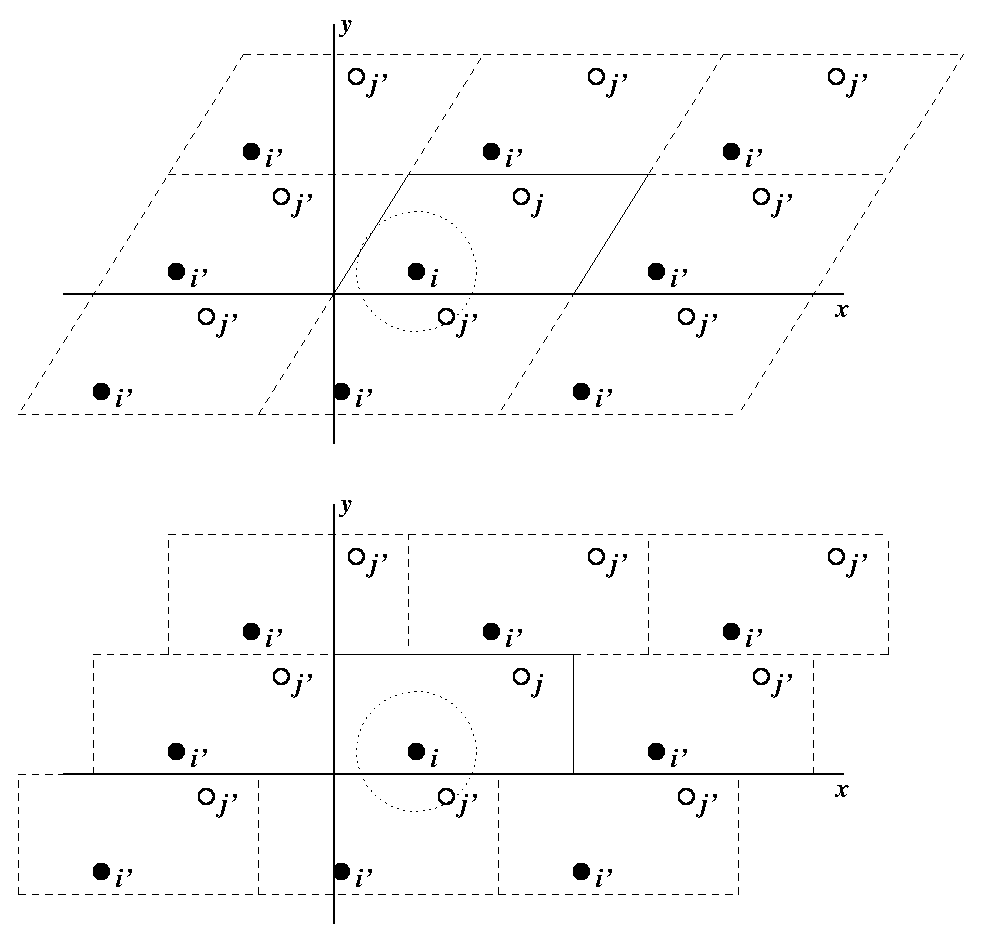
\includegraphics[width=9cm]{plots/pbctric}}
\caption {Periodic boundary conditions in two dimensions.}
\label{fig:pbc}
\end{figure}
The classical way to minimize edge effects in a finite system is to
apply {\em periodic boundary conditions}. The atoms of the system to
be simulated are put into a space-filling box, which is surrounded by
translated copies of itself (\figref{pbc}).  Thus there are no
boundaries of the system; the artifact caused by unwanted boundaries
in an isolated cluster is now replaced by the artifact of periodic
conditions. If the system is crystalline, such boundary conditions are
desired (although motions are naturally restricted to periodic motions
with wavelengths fitting into the box). If one wishes to simulate
non-periodic systems, such as liquids or solutions, the periodicity by
itself causes errors. The errors can be evaluated by comparing various
system sizes; they are expected to be less severe than the errors
resulting from an unnatural boundary with vacuum.

There are several possible shapes for space-filling unit cells. Some,
like the {\em \normindex{rhombic dodecahedron}} and the
{\em \normindex{truncated octahedron}}~\cite{Adams79} are closer to being a sphere
than a cube is, and are therefore better suited to the 
study of an approximately spherical macromolecule in solution, since
fewer solvent molecules are required to fill the box given a minimum
distance between macromolecular images. At the same time, rhombic 
dodecahedra and truncated octahedra are special cases of {\em triclinic} 
unit cells\index{triclinic unit cell}; the most general space-filling unit cells
that comprise all possible space-filling shapes~\cite{Bekker95}.
For this reason, {\gromacs} is based on the triclinic unit cell.
  
{\gromacs} uses periodic boundary conditions, combined with the {\em
\normindex{minimum image convention}}: only one -- the nearest -- image of each
particle is considered for short-range non-bonded interaction terms.
For long-range electrostatic interactions this is not always accurate
enough, and {\gromacs} therefore also incorporates lattice sum methods
such as Ewald Sum, PME and PPPM.

{\gromacs} supports triclinic boxes of any shape.
The simulation box (unit cell) is defined by the 3 box vectors 
${\bf a}$,${\bf b}$ and ${\bf c}$.
The box vectors must satisfy the following conditions:
\beq
\label{eqn:box_rot}
a_y = a_z = b_z = 0
\eeq
\beq
\label{eqn:box_shift1}
a_x>0,~~~~b_y>0,~~~~c_z>0
\eeq
\beq
\label{eqn:box_shift2}
|b_x| \leq \frac{1}{2} \, a_x,~~~~
|c_x| \leq \frac{1}{2} \, a_x,~~~~
|c_y| \leq \frac{1}{2} \, b_y
\eeq
Equations \ref{eqn:box_rot} can always be satisfied by rotating the box.
Inequalities (\ref{eqn:box_shift1}) and (\ref{eqn:box_shift2}) can always be
satisfied by adding and subtracting box vectors.

Even when simulating using a triclinic box, {\gromacs} always keeps the
particles in a brick-shaped volume for efficiency,
as illustrated in \figref{pbc} for a 2-dimensional system.
Therefore, from the output trajectory it might seem that the simulation was
done in a rectangular box. The program {\tt trjconv} can be used to convert 
the trajectory to a different unit-cell representation.

It is also possible to simulate without periodic boundary conditions,
but it is usually more efficient to simulate an isolated cluster of molecules
in a large periodic box, since fast grid searching can only be used 
in a periodic system.

\begin{figure}
\centerline{
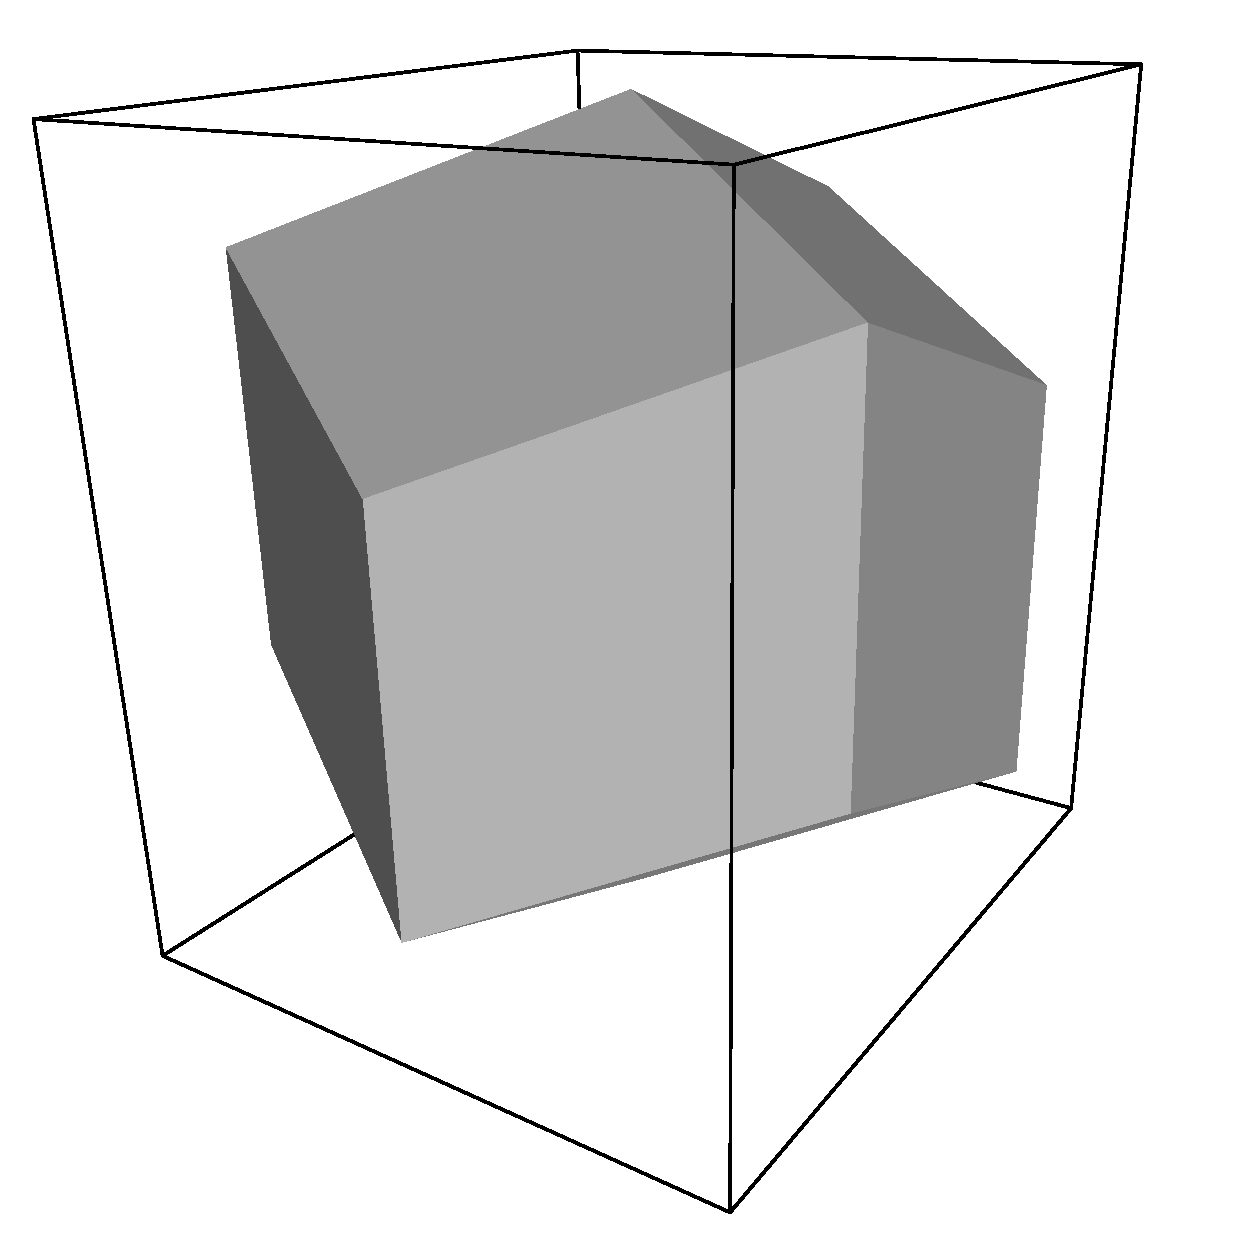
\includegraphics[width=5cm]{plots/rhododec}
~~~~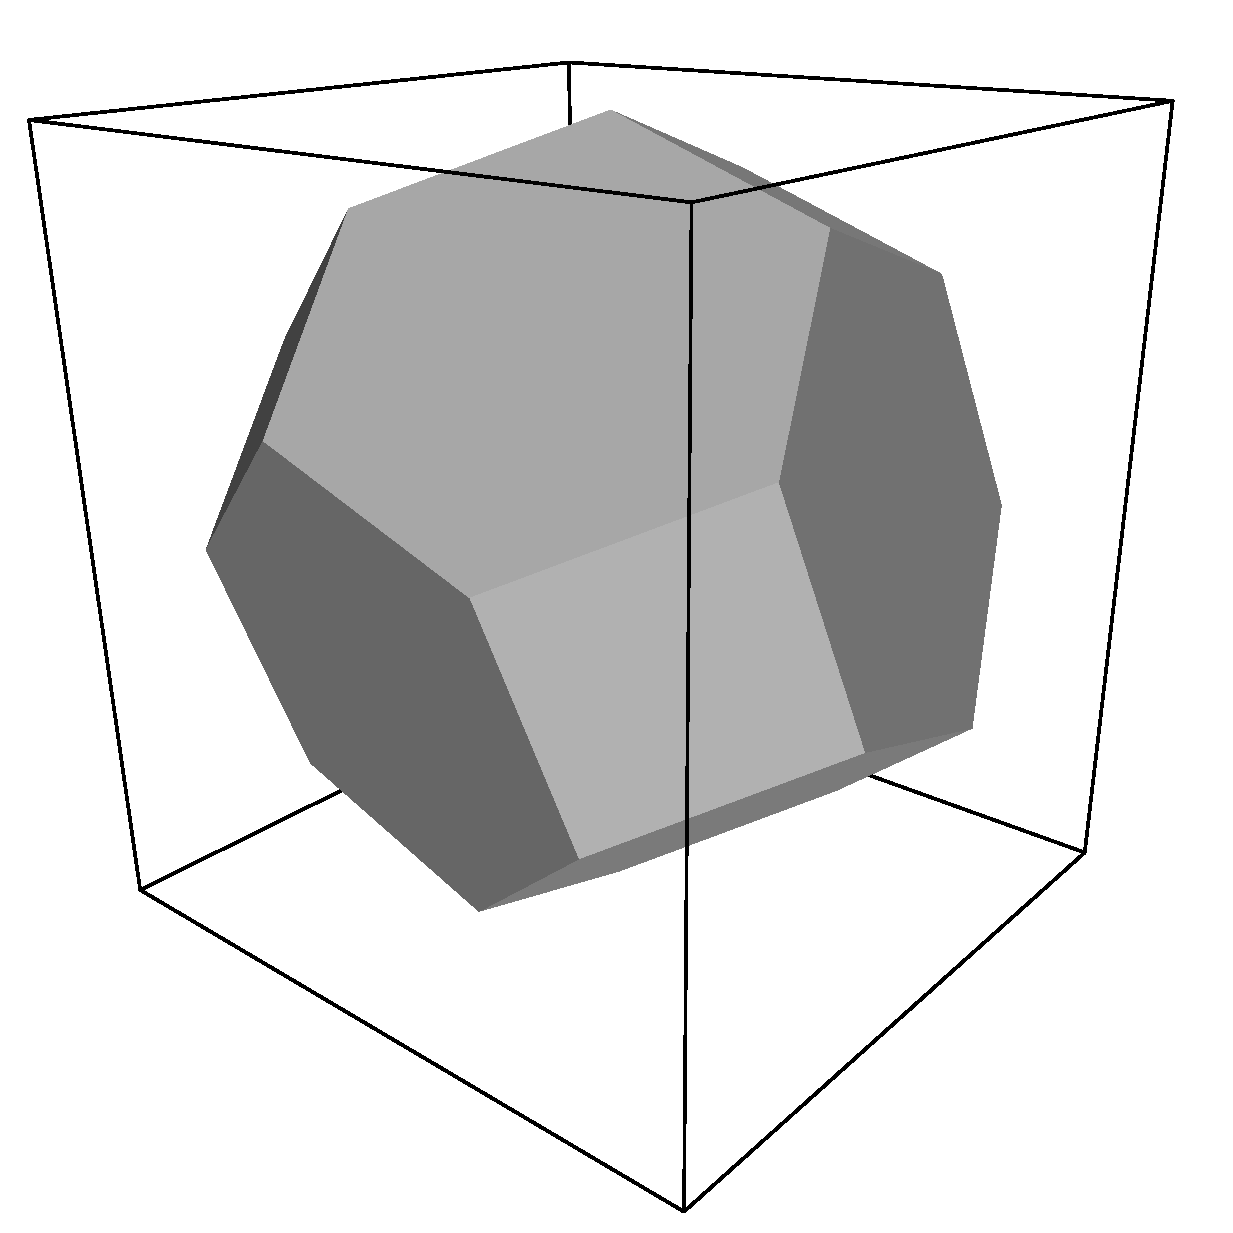
\includegraphics[width=5cm]{plots/truncoct}
}
\caption {A rhombic dodecahedron and truncated octahedron
(arbitrary orientations).}
\label{fig:boxshapes}
\end{figure}

\subsection{Some useful box types}
\begin{table}
\centerline{
\begin{tabular}{|c|c|c|ccc|ccc|}
\dline
box type & image & box & \multicolumn{3}{c|}{box vectors} & \multicolumn{3}{c|}{box vector angles} \\
 & distance & volume & ~{\bf a}~ & {\bf b} & {\bf c} &
   $\angle{\bf bc}$ & $\angle{\bf ac}$ & $\angle{\bf ab}$ \\
\dline
             &     &       & $d$ & 0              & 0              & & & \\
cubic        & $d$ & $d^3$ & 0   & $d$            & 0              & $90^\circ$ & $90^\circ$ & $90^\circ$ \\
             &     &       & 0   & 0              & $d$            & & & \\
\hline
rhombic      &     &       & $d$ & 0              & $\frac{1}{2}\,d$ & & & \\
dodecahedron & $d$ & $\frac{1}{2}\sqrt{2}\,d^3$ & 0   & $d$            & $\frac{1}{2}\,d$ & $60^\circ$ & $60^\circ$ & $90^\circ$ \\
(xy-square)  &     & $0.707\,d^3$ & 0   & 0              & $\frac{1}{2}\sqrt{2}\,d$ & & & \\
\hline
rhombic      &     &       & $d$ & $\frac{1}{2}\,d$ & $\frac{1}{2}\,d$ & & & \\
dodecahedron & $d$ & $\frac{1}{2}\sqrt{2}\,d^3$ & 0 & $\frac{1}{2}\sqrt{3}\,d$ & $\frac{1}{6}\sqrt{3}\,d$ & $60^\circ$ & $60^\circ$ & $60^\circ$ \\
(xy-hexagon) &     & $0.707\,d^3$ & 0   & 0              & $\frac{1}{3}\sqrt{6}\,d$ & & & \\
\hline
truncated    &     &       & $d$ & $\frac{1}{3}\,d$ & $-\frac{1}{3}\,d$ & & &\\
octahedron   & $d$ & $\frac{4}{9}\sqrt{3}\,d^3$ & 0   & $\frac{2}{3}\sqrt{2}\,d$ & $\frac{1}{3}\sqrt{2}\,d$ & $71.53^\circ$ & $109.47^\circ$ & $71.53^\circ$ \\
             &     & $0.770\,d^3$ & 0   & 0              & $\frac{1}{3}\sqrt{6}\,d$ & & & \\
\dline
\end{tabular}
}
\caption{The cubic box, the rhombic \normindex{dodecahedron} and the truncated
\normindex{octahedron}.}
\label{tab:boxtypes}
\end{table}
The three most useful box types for simulations of solvated systems
are described in \tabref{boxtypes}.  The rhombic dodecahedron
(\figref{boxshapes}) is the smallest and most regular space-filling
unit cell. Each of the 12 image cells is at the same distance.  The
volume is 71\% of the volume of a cube having the same image
distance. This saves about 29\% of CPU-time when simulating a
spherical or flexible molecule in solvent. There are two different
orientations of a rhombic dodecahedron that satisfy equations
\ref{eqn:box_rot}, \ref{eqn:box_shift1} and \ref{eqn:box_shift2}.
The program {\tt editconf} produces the orientation
which has a square intersection with the xy-plane.  This orientation
was chosen because the first two box vectors coincide with the x and
y-axis, which is easier to comprehend. The other orientation can be
useful for simulations of membrane proteins. In this case the
cross-section with the xy-plane is a hexagon, which has an area which
is 14\% smaller than the area of a square with the same image
distance.  The height of the box ($c_z$) should be changed to obtain
an optimal spacing.  This box shape not only saves CPU time, it
also results in a more uniform arrangement of the proteins.

\subsection{Cut-off restrictions}
The \normindex{minimum image convention} implies that the cut-off radius used to
truncate non-bonded interactions may not exceed half the shortest box
vector:
\beq
\label{eqn:physicalrc}
  R_c < \half \min(\|{\bf a}\|,\|{\bf b}\|,\|{\bf c}\|),
\eeq
because otherwise more than one image would be within the cut-off distance 
of the force. When a macromolecule, such as a protein, is studied in
solution, this restriction alone is not sufficient: in principle, a single
solvent molecule should not be able
to `see' both sides of the macromolecule. This means that the length of
each box vector must exceed the length of the macromolecule in the
direction of that edge {\em plus} two times the cut-off radius $R_c$.
It is, however, common to compromise in this respect, and make the solvent 
layer somewhat smaller in order to reduce the computational cost.
For efficiency reasons the cut-off with triclinic boxes is more restricted.
For grid search the extra restriction is weak:
\beq
\label{eqn:gridrc}
R_c < \min(a_x,b_y,c_z)
\eeq
For simple search the extra restriction is stronger:
\beq
\label{eqn:simplerc}
R_c < \half \min(a_x,b_y,c_z)
\eeq

Each unit cell (cubic, rectangular or triclinic)
is surrounded by 26 translated images. A
particular image can therefore always be identified by an index pointing to one
of 27 {\em translation vectors} and constructed by applying a
translation with the indexed vector (see \ssecref{forces}).
Restriction (\ref{eqn:gridrc}) ensures that only 26 images need to be
considered.

%\ifthenelse{\equal{\gmxlite}{1}}{}{
\section{The group concept}
\label{sec:groupconcept}\index{group}
The {\gromacs} MD and analysis programs use user-defined {\em groups} of
atoms to perform certain actions on. The maximum number of groups is
256, but each atom can only belong to six different groups, one 
each of the following:
\begin{description}
\item[\swapindex{temperature-coupling}{group}]
The \normindex{temperature coupling} parameters (reference
temperature, time constant, number of degrees of freedom, see
\ssecref{update}) can be defined for each T-coupling group
separately. For example, in a solvated macromolecule the solvent (that
tends to generate more heating by force and integration errors) can be
coupled with a shorter time constant to a bath than is a macromolecule,
or a surface can be kept cooler than an adsorbing molecule. Many
different T-coupling groups may be defined. See also center of mass
groups below.

\item[\swapindex{freeze}{group}\index{frozen atoms}]
Atoms that belong to a freeze group are kept stationary in the
dynamics. This is useful during equilibration, {\eg} to avoid badly
placed solvent molecules giving unreasonable kicks to protein atoms,
although the same effect can also be obtained by putting a restraining
potential on the atoms that must be protected. The freeze option can
be used, if desired, on just one or two coordinates of an atom,
thereby freezing the atoms in a plane or on a line.  When an atom is
partially frozen, constraints will still be able to move it, even in a
frozen direction. A fully frozen atom can not be moved by constraints.
Many freeze groups can be defined.  Frozen coordinates are unaffected
by pressure scaling; in some cases this can produce unwanted results,
particularly when constraints are also used (in this case you will
get very large pressures). Accordingly, it is recommended to avoid
combining freeze groups with constraints and pressure coupling. For the
sake of equilibration it could suffice to start with freezing in a
constant volume simulation, and afterward use position restraints in
conjunction with constant pressure.

\item[\swapindex{accelerate}{group}]
On each atom in an ``accelerate group'' an acceleration
$\ve{a}^g$ is imposed. This is equivalent to an external
force. This feature makes it possible to drive the system into a
non-equilibrium state and enables the performance of 
\swapindex{non-equilibrium}{MD} and hence to obtain transport properties.

\item[\swapindex{energy-monitor}{group}]
Mutual interactions between all energy-monitor groups are compiled
during the simulation. This is done separately for Lennard-Jones and
Coulomb terms.  In principle up to 256 groups could be defined, but
that would lead to 256$\times$256 items! Better use this concept
sparingly.

All non-bonded interactions between pairs of energy-monitor groups can
be excluded\index{exclusions}
\ifthenelse{\equal{\gmxlite}{1}}
{.}
{(see details in the User Guide).}
Pairs of particles from excluded pairs of energy-monitor groups
are not put into the pair list.
This can result in a significant speedup
for simulations where interactions within or between parts of the system
are not required.

\item[\swapindex{center of mass}{group}\index{removing COM motion}]
In \gromacs\ the center of mass (COM) motion can be removed, for
either the complete system or for groups of atoms. The latter is
useful, {\eg} for systems where there is limited friction ({\eg} gas
systems) to prevent center of mass motion to occur. It makes sense to
use the same groups for temperature coupling and center of mass motion
removal.

\item[\swapindex{Compressed position output}{group}]

In order to further reduce the size of the compressed trajectory file
({\tt .xtc{\index{XTC}}} or {\tt .tng{\index{TNG}}}), it is possible
to store only a subset of all particles. All x-compression groups that
are specified are saved, the rest are not. If no such groups are
specified, than all atoms are saved to the compressed trajectory file.

\end{description}
The use of groups in {\gromacs} tools is described in
\secref{usinggroups}.
%} % Brace matches ifthenelse test for gmxlite

\section{Molecular Dynamics}
\label{sec:MD}
\begin{figure}
\begin{center}
\addtolength{\fboxsep}{0.5cm}
\begin{shadowenv}[12cm]
{\large \bf THE GLOBAL MD ALGORITHM}
\rule{\textwidth}{2pt} \\
{\bf 1. Input initial conditions}\\[2ex]
Potential interaction $V$ as a function of atom positions\\
Positions $\ve{r}$ of all atoms in the system\\
Velocities $\ve{v}$ of all atoms in the system \\
$\Downarrow$\\
\rule{\textwidth}{1pt}\\
{\bf repeat 2,3,4} for the required number of steps:\\
\rule{\textwidth}{1pt}\\
{\bf 2. Compute forces} \\[1ex]
The force on any atom  \\[1ex]
$\ve{F}_i = - \displaystyle\frac{\partial V}{\partial \ve{r}_i}$ \\[1ex]
is computed by calculating the force between non-bonded atom pairs: \\
$\ve{F}_i = \sum_j \ve{F}_{ij}$ \\
plus the forces due to bonded interactions (which may depend on 1, 2,
3, or 4 atoms), plus restraining and/or external forces. \\
The potential and kinetic energies and the pressure tensor may be computed. \\
$\Downarrow$\\
{\bf 3. Update configuration} \\[1ex]
The movement of the atoms is simulated by numerically solving Newton's
equations of motion \\[1ex]
$\displaystyle
\frac {\de^2\ve{r}_i}{\de t^2} = \frac{\ve{F}_i}{m_i} $ \\
or \\
$\displaystyle
\frac{\de\ve{r}_i}{\de t} = \ve{v}_i ; \;\;
\frac{\de\ve{v}_i}{\de t} = \frac{\ve{F}_i}{m_i} $ \\[1ex]
$\Downarrow$ \\
{\bf 4.} if required: {\bf Output step} \\
write positions, velocities, energies, temperature, pressure, etc. \\
\end{shadowenv}
\caption{The global MD algorithm}
\label{fig:global}
\end{center}
\end{figure}
A global flow scheme for MD is given in \figref{global}. Each
MD or  EM run requires as input a set of initial coordinates and --
optionally -- initial velocities of all particles involved. This
chapter does not describe how these are obtained; for the setup of an
actual MD run check the online manual at {\wwwpage}.

\subsection{Initial conditions}
\subsubsection{Topology and force field}
The system topology, including a description of the force field, must
be read in.
\ifthenelse{\equal{\gmxlite}{1}}
{.}
{Force fields and topologies are described in \chref{ff}
and \ref{ch:top}, respectively.}
All this information is static; it is never modified during the run.

\subsubsection{Coordinates and velocities}
\begin{figure}
\centerline{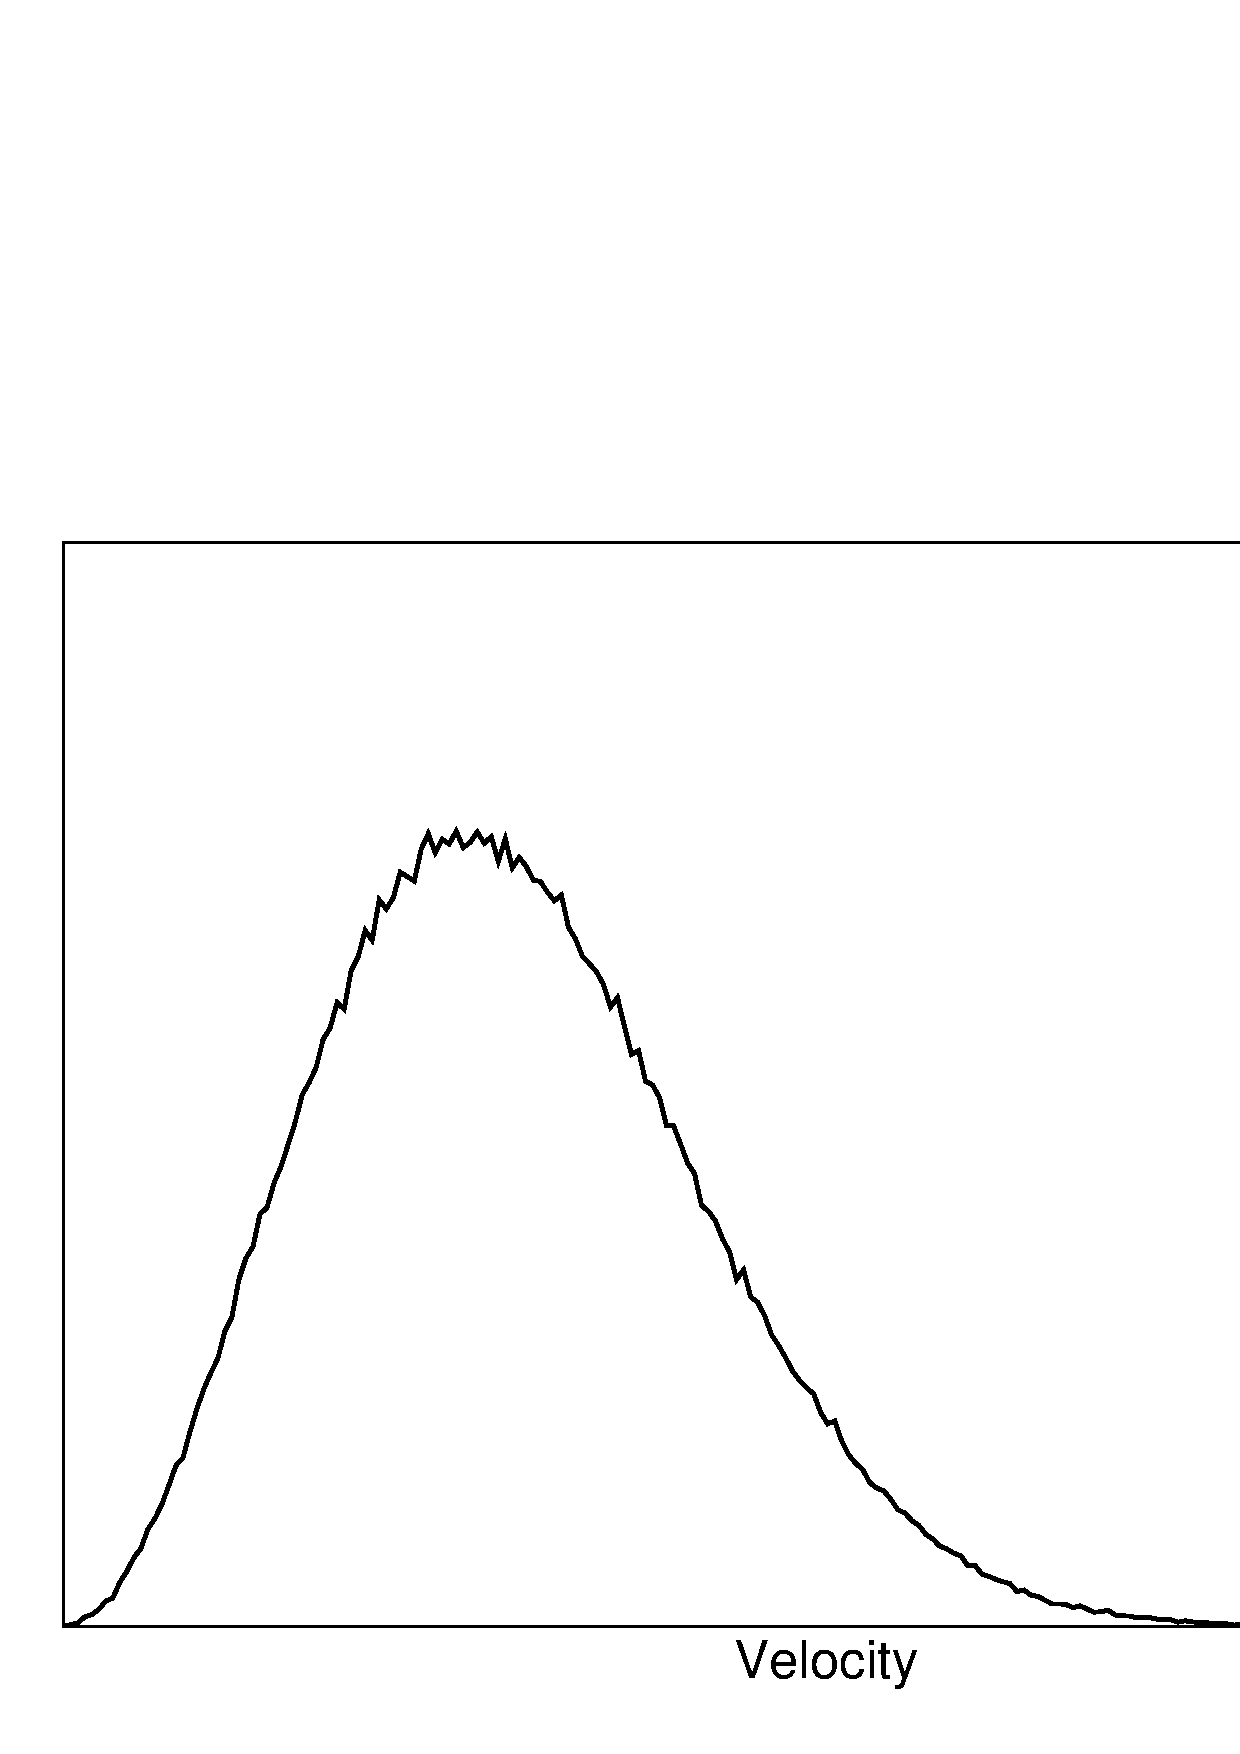
\includegraphics[width=8cm]{plots/maxwell}}
\caption{A Maxwell-Boltzmann velocity distribution, generated from 
    random numbers.}
\label{fig:maxwell}
\end{figure}

Then, before a run starts, the box size and the coordinates and
velocities of  all particles are required. The box size and shape is 
determined by three vectors (nine numbers) $\ve{b}_1, \ve{b}_2, \ve{b}_3$, 
which represent the three basis vectors of the periodic box.

If the run starts at $t=t_0$, the coordinates at $t=t_0$ must be
known. The {\em leap-frog algorithm}, the default algorithm used to 
update the time step with $\Dt$ (see \ssecref{update}), also requires 
that the velocities at $t=t_0 - \hDt$ are known. If velocities are not 
available, the program can generate initial atomic velocities 
$v_i, i=1\ldots 3N$ with a \index{Maxwell-Boltzmann distribution} 
(\figref{maxwell}) at a given absolute temperature $T$:
\beq 
p(v_i) = \sqrt{\frac{m_i}{2 \pi kT}}\exp\left(-\frac{m_i v_i^2}{2kT}\right)
\eeq
where $k$ is Boltzmann's constant (see \chref{defunits}).
To accomplish this, normally distributed random numbers are generated
by adding twelve random numbers $R_k$ in the range $0 \le R_k < 1$ and
subtracting 6.0 from their sum. The result is then multiplied by the
standard deviation of the velocity distribution $\sqrt{kT/m_i}$. Since
the resulting total energy will not correspond exactly to the required
temperature $T$, a correction is made: first the center-of-mass motion
is removed and then all velocities are scaled so that the total
energy corresponds exactly to $T$ (see \eqnref{E-T}). 
% Why so complicated? What's wrong with Box-Mueller transforms?

\subsubsection{Center-of-mass motion\index{removing COM motion}}
The \swapindex{center-of-mass}{velocity} is normally set to zero at
every step; there is (usually) no net external force acting on the
system and the center-of-mass velocity should remain constant. In
practice, however, the update algorithm introduces a very slow change in
the center-of-mass velocity, and therefore in the total kinetic energy of
the system -- especially when temperature coupling is used. If such
changes are not quenched, an appreciable center-of-mass motion
can develop in long runs, and the temperature will be
significantly misinterpreted. Something similar may happen due to overall
rotational motion, but only when an isolated cluster is simulated. In
periodic systems with filled boxes, the overall rotational motion is
coupled to other degrees of freedom and does not cause such problems.


\subsection{Neighbor searching\swapindexquiet{neighbor}{searching}}
\label{subsec:ns}
As mentioned in \chref{ff}, internal forces are
either generated from fixed (static) lists, or from dynamic lists.
The latter consist of non-bonded interactions between any pair of particles.
When calculating the non-bonded forces, it is convenient to have all
particles in a rectangular box.
As shown in \figref{pbc}, it is possible to transform a
triclinic box into a rectangular box.
The output coordinates are always in a rectangular box, even when a
dodecahedron or triclinic box was used for the simulation.
Equation \ref{eqn:box_rot} ensures that we can reset particles
in a rectangular box by first shifting them with
box vector ${\bf c}$, then with ${\bf b}$ and finally with ${\bf a}$.
Equations \ref{eqn:box_shift2}, \ref{eqn:physicalrc} and \ref{eqn:gridrc}
ensure that we can find the 14 nearest triclinic images within
a linear combination that does not involve multiples of box vectors.

\subsubsection{Pair lists generation}
The non-bonded pair forces need to be calculated only for those pairs
$i,j$  for which the distance $r_{ij}$ between $i$ and the 
\swapindex{nearest}{image} 
of $j$ is less than a given cut-off radius $R_c$. Some of the particle
pairs that fulfill this criterion are excluded, when their interaction
is already fully accounted for by bonded interactions.  {\gromacs}
employs a {\em pair list} that contains those particle pairs for which
non-bonded forces must be calculated.  The pair list contains particles
$i$, a displacement vector for particle $i$, and all particles $j$ that
are within \verb'rlist' of this particular image of particle $i$.  The
list is updated every \verb'nstlist' steps.

To make the \normindex{neighbor list}, all particles that are close
({\ie} within the neighbor list cut-off) to a given particle must be found.
This searching, usually called neighbor search (NS) or pair search,
involves periodic boundary conditions and determining the {\em image}
(see \secref{pbc}). The search algorithm is $O(N)$, although a simpler
$O(N^2)$ algorithm is still available under some conditions.

\subsubsection{\normindex{Cut-off schemes}: group versus Verlet}
From version 4.6, {\gromacs} supports two different cut-off scheme
setups: the original one based on particle groups and one using a Verlet
buffer. There are some important differences that affect results,
performance and feature support. The group scheme can be made to work
(almost) like the Verlet scheme, but this will lead to a decrease in
performance. The group scheme is especially fast for water molecules,
which are abundant in many simulations, but on the most recent x86
processors, this advantage is negated by the better instruction-level
parallelism available in the Verlet-scheme implementation. The group
scheme is deprecated in version 5.0, and will be removed in a future
version. For practical details of choosing and setting up
cut-off schemes, please see the User Guide.

In the group scheme, a neighbor list is generated consisting of pairs
of groups of at least one particle. These groups were originally
\swapindex{charge}{group}s \ifthenelse{\equal{\gmxlite}{1}}{}{(see
  \secref{chargegroup})}, but with a proper treatment of long-range
electrostatics, performance in unbuffered simulations is their only advantage. A pair of groups
is put into the neighbor list when their center of geometry is within
the cut-off distance. Interactions between all particle pairs (one from
each charge group) are calculated for a certain number of MD steps,
until the neighbor list is updated. This setup is efficient, as the
neighbor search only checks distance between charge-group pair, not
particle pairs (saves a factor of $3 \times 3 = 9$ with a three-particle water
model) and the non-bonded force kernels can be optimized for, say, a
water molecule ``group''. Without explicit buffering, this setup leads
to energy drift as some particle pairs which are within the cut-off don't
interact and some outside the cut-off do interact. This can be caused
by
\begin{itemize}
\item particles moving across the cut-off between neighbor search steps, and/or
\item for charge groups consisting of more than one particle, particle pairs
  moving in/out of the cut-off when their charge group center of
  geometry distance is outside/inside of the cut-off.
\end{itemize}
Explicitly adding a buffer to the neighbor list will remove such
artifacts, but this comes at a high computational cost. How severe the
artifacts are depends on the system, the properties in which you are
interested, and the cut-off setup.

The Verlet cut-off scheme uses a buffered pair list by default. It
also uses clusters of particles, but these are not static as in the group
scheme. Rather, the clusters are defined spatially and consist of 4 or
8 particles, which is convenient for stream computing, using e.g. SSE, AVX
or CUDA on GPUs. At neighbor search steps, a pair list is created
with a Verlet buffer, ie. the pair-list cut-off is larger than the
interaction cut-off. In the non-bonded kernels, interactions are only
computed when a particle pair is within the cut-off distance at that
particular time step. This ensures that as particles move between pair
search steps, forces between nearly all particles within the cut-off
distance are calculated. We say {\em nearly} all particles, because
{\gromacs} uses a fixed pair list update frequency for
efficiency. A particle-pair, whose distance was outside the cut-off,
could possibly move enough during this fixed number of
steps that its distance is now within the cut-off. This
small chance results in a small energy drift, and the size of the
chance depends on the temperature. When temperature
coupling is used, the buffer size can be determined automatically,
given a certain tolerance on the energy drift.

The Verlet cut-off scheme is implemented in a very efficient fashion
based on clusters of particles. The simplest example is a cluster size
of 4 particles. The pair list is then constructed based on cluster
pairs. The cluster-pair search is much faster searching based on
particle pairs, because $4 \times 4 = 16$ particle pairs are put in
the list at once. The non-bonded force calculation kernel can then
calculate many particle-pair interactions at once, which maps nicely
to SIMD or SIMT units on modern hardware, which can perform multiple
floating operations at once. These non-bonded kernels
are much faster than the kernels used in the group scheme for most
types of systems, particularly on newer hardware.

Additionally, when the list buffer is determined automatically as
described below, we also apply dynamic pair list pruning. The pair list
can be constructed infrequently, but that can lead to a lot of pairs
in the list that are outside the cut-off range for all or most of
the life time of this pair list. Such pairs can be pruned out by
applying a cluster-pair kernel that only determines which clusters
are in range. Because of the way the non-bonded data is regularized
in {\gromacs}, this kernel is an order of magnitude faster than
the search and the interaction kernel. On the GPU this pruning is
overlapped with the integration on the CPU, so it is free in most
cases. Therefore we can prune every 4-10 integration steps with
little overhead and significantly reduce the number of cluster pairs
in the interaction kernel. This procedure is applied automatically,
unless the user set the pair-list buffer size manually.

\ifthenelse{\equal{\gmxlite}{1}}{}{
\subsubsection{Energy drift and pair-list buffering}
For a canonical (NVT) ensemble, the average energy error caused by
diffusion of $j$ particles from outside the pair-list cut-off
$r_\ell$ to inside the interaction cut-off $r_c$ over the lifetime
of the list can be determined from the atomic
displacements and the shape of the potential at the cut-off.
%Since we are interested in the small drift regime, we will assume
%#that atoms will only move within the cut-off distance in the last step,
%$n_\mathrm{ps}-1$, of the pair list update interval $n_\mathrm{ps}$.
%Over this number of steps the displacment of an atom with mass $m$
The displacement distribution along one dimension for a freely moving
particle with mass $m$ over time $t$ at temperature $T$ is
a Gaussian $G(x)$
of zero mean and variance $\sigma^2 = t^2 k_B T/m$. For the distance
between two particles, the variance changes to $\sigma^2 = \sigma_{12}^2 =
t^2 k_B T(1/m_1+1/m_2)$. Note that in practice particles usually
interact with (bump into) other particles over time $t$ and therefore the real
displacement distribution is much narrower.  Given a non-bonded
interaction cut-off distance of $r_c$ and a pair-list cut-off
$r_\ell=r_c+r_b$ for $r_b$ the Verlet buffer size, we can then
write the average energy error after time $t$ for all missing pair
interactions between a single $i$ particle of type 1 surrounded
by all $j$ particles that are of type 2 with number density $\rho_2$,
when the inter-particle distance changes from $r_0$ to $r_t$, as:
\beq
\langle \Delta V \rangle =
\int_{0}^{r_c} \int_{r_\ell}^\infty 4 \pi r_0^2 \rho_2 V(r_t) G\!\left(\frac{r_t-r_0}{\sigma}\right) d r_0\, d r_t
\eeq
To evaluate this analytically, we need to make some approximations. First we replace $V(r_t)$ by a Taylor expansion around $r_c$, then we can move the lower bound of the integral over $r_0$ to $-\infty$ which will simplify the result:
\begin{eqnarray}
\langle \Delta V \rangle &\approx&
\int_{-\infty}^{r_c} \int_{r_\ell}^\infty 4 \pi r_0^2 \rho_2 \Big[ V'(r_c) (r_t - r_c) +
\nonumber\\
& &
\phantom{\int_{-\infty}^{r_c} \int_{r_\ell}^\infty 4 \pi r_0^2 \rho_2 \Big[}
V''(r_c)\frac{1}{2}(r_t - r_c)^2 +
\nonumber\\
& &
\phantom{\int_{-\infty}^{r_c} \int_{r_\ell}^\infty 4 \pi r_0^2 \rho_2 \Big[}
  V'''(r_c)\frac{1}{6}(r_t - r_c)^3 +
  \nonumber\\
& &
\phantom{\int_{-\infty}^{r_c} \int_{r_\ell}^\infty 4 \pi r_0^2 \rho_2 \Big[}
  O \! \left((r_t - r_c)^4 \right)\Big] G\!\left(\frac{r_t-r_0}{\sigma}\right) d r_0 \, d r_t
\end{eqnarray}
Replacing the factor $r_0^2$ by $(r_\ell + \sigma)^2$, which results in a slight overestimate, allows us to calculate the integrals analytically:
\begin{eqnarray}
\langle \Delta V \rangle \!
&\approx&
4 \pi (r_\ell+\sigma)^2 \rho_2
\int_{-\infty}^{r_c} \int_{r_\ell}^\infty \Big[ V'(r_c) (r_t - r_c) +
\nonumber\\
& &
\phantom{4 \pi (r_\ell+\sigma)^2 \rho_2 \int_{-\infty}^{r_c} \int_{r_\ell}^\infty \Big[}
V''(r_c)\frac{1}{2}(r_t - r_c)^2 +
\nonumber\\
& &
\phantom{4 \pi (r_\ell+\sigma)^2 \rho_2 \int_{-\infty}^{r_c} \int_{r_\ell}^\infty \Big[}
V'''(r_c)\frac{1}{6}(r_t - r_c)^3 \Big] G\!\left(\frac{r_t-r_0}{\sigma}\right)
d r_0 \, d r_t\\
&=&
4 \pi (r_\ell+\sigma)^2 \rho_2 \bigg\{
\frac{1}{2}V'(r_c)\left[r_b \sigma G\!\left(\frac{r_b}{\sigma}\right) - (r_b^2+\sigma^2)E\!\left(\frac{r_b}{\sigma}\right) \right] +
\nonumber\\
& &
\phantom{4 \pi (r_\ell+\sigma)^2 \rho_2 \bigg\{ }
\frac{1}{6}V''(r_c)\left[ \sigma(r_b^2+2\sigma^2) G\!\left(\frac{r_b}{\sigma}\right) - r_b(r_b^2+3\sigma^2 ) E\!\left(\frac{r_b}{\sigma}\right) \right] +
\nonumber\\
& &
\phantom{4 \pi (r_\ell+\sigma)^2 \rho_2 \bigg\{ }
\frac{1}{24}V'''(r_c)\bigg[ r_b\sigma(r_b^2+5\sigma^2) G\!\left(\frac{r_b}{\sigma}\right)
\nonumber\\
& &
\phantom{4 \pi (r_\ell+\sigma)^2 \rho_2 \bigg\{ \frac{1}{24}V'''(r_c)\bigg[ }
 - (r_b^4+6r_b^2\sigma^2+3\sigma^4 ) E\!\left(\frac{r_b}{\sigma}\right) \bigg]
\bigg\}
\end{eqnarray}

where $G(x)$ is a Gaussian distribution with 0 mean and unit variance and
$E(x)=\frac{1}{2}\mathrm{erfc}(x/\sqrt{2})$. We always want to achieve
small energy error, so $\sigma$ will be small compared to both $r_c$
and $r_\ell$, thus the approximations in the equations above are good,
since the Gaussian distribution decays rapidly. The energy error needs
to be averaged over all particle pair types and weighted with the
particle counts. In {\gromacs} we don't allow cancellation of error
between pair types, so we average the absolute values. To obtain the
average energy error per unit time, it needs to be divided by the
neighbor-list life time $t = ({\tt nstlist} - 1)\times{\tt dt}$. The
function can not be inverted analytically, so we use bisection to
obtain the buffer size $r_b$ for a target drift.  Again we note that
in practice the error we usually be much smaller than this estimate,
as in the condensed phase particle displacements will be much smaller
than for freely moving particles, which is the assumption used here.

When (bond) constraints are present, some particles will have fewer
degrees of freedom. This will reduce the energy errors. For simplicity,
we only consider one constraint per particle, the heaviest particle
in case a particle is involved in multiple constraints.
This simplification overestimates the displacement. The motion of
a constrained particle is a superposition of the 3D motion of the
center of mass of both particles and a 2D rotation around the center of mass.
The displacement in an arbitrary direction of a particle with 2 degrees
of freedom is not Gaussian, but rather follows the complementary error
function:
\beq
\frac{\sqrt{\pi}}{2\sqrt{2}\sigma}\,\mathrm{erfc}\left(\frac{|r|}{\sqrt{2}\,\sigma}\right)
\label{eqn:2D_disp}
\eeq
where $\sigma^2$ is again $t^2 k_B T/m$.  This distribution can no
longer be integrated analytically to obtain the energy error. But we
can generate a tight upper bound using a scaled and shifted Gaussian
distribution (not shown). This Gaussian distribution can then be used
to calculate the energy error as described above. The rotation displacement
around the center of mass can not be more than the length of the arm.
To take this into account, we scale $\sigma$ in \eqnref{2D_disp} (details
not presented here) to obtain an overestimate of the real displacement.
This latter effect significantly reduces the buffer size for longer
neighborlist lifetimes in e.g. water, as constrained hydrogens are by far
the fastest particles, but they can not move further than 0.1 nm
from the heavy atom they are connected to.


There is one important implementation detail that reduces the energy
errors caused by the finite Verlet buffer list size. The derivation
above assumes a particle pair-list. However, the {\gromacs}
implementation uses a cluster pair-list for efficiency. The pair list
consists of pairs of clusters of 4 particles in most cases, also
called a $4 \times 4$ list, but the list can also be $4 \times 8$ (GPU
CUDA kernels and AVX 256-bit single precision kernels) or $4 \times 2$
(SSE double-precision kernels). This means that the pair-list is
effectively much larger than the corresponding $1 \times 1$ list. Thus
slightly beyond the pair-list cut-off there will still be a large
fraction of particle pairs present in the list. This fraction can be
determined in a simulation and accurately estimated under some
reasonable assumptions. The fraction decreases with increasing
pair-list range, meaning that a smaller buffer can be used. For
typical all-atom simulations with a cut-off of 0.9 nm this fraction is
around 0.9, which gives a reduction in the energy errors of a factor of
10. This reduction is taken into account during the automatic Verlet
buffer calculation and results in a smaller buffer size.

\begin{figure}
\centerline{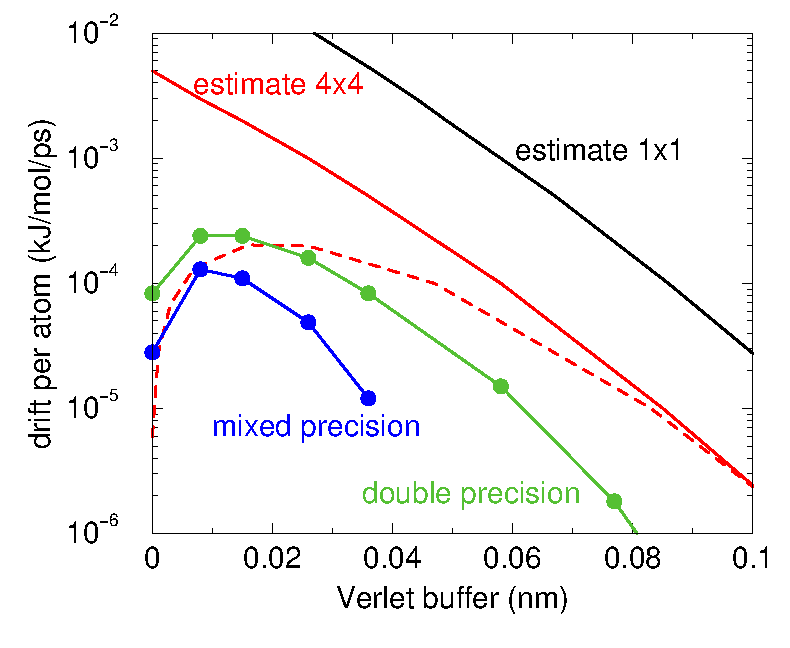
\includegraphics[width=9cm]{plots/verlet-drift}}
\caption {Energy drift per atom for an SPC/E water system at 300K with
  a time step of 2 fs and a pair-list update period of 10 steps
  (pair-list life time: 18 fs). PME was used with {\tt ewald-rtol} set
  to 10$^{-5}$; this parameter affects the shape of the potential at
  the cut-off. Error estimates due to finite Verlet buffer size are
  shown for a $1 \times 1$ atom pair list and $4 \times 4$ atom pair
  list without and with (dashed line) cancellation of positive and
  negative errors. Real energy drift is shown for simulations using
  double- and mixed-precision settings. Rounding errors in the SETTLE
  constraint algorithm from the use of single precision causes
  the drift to become negative
  at large buffer size. Note that at zero buffer size, the real drift
  is small because positive (H-H) and negative (O-H) energy errors
  cancel.}
\label{fig:verletdrift}
\end{figure}

In \figref{verletdrift} one can see that for small buffer sizes the drift
of the total energy is much smaller than the pair energy error tolerance,
due to cancellation of errors. For larger buffer size, the error estimate
is a factor of 6 higher than drift of the total energy, or alternatively
the buffer estimate is 0.024 nm too large. This is because the protons
don't move freely over 18 fs, but rather vibrate.
%At a buffer size of zero there is cancellation of
%drift due to repulsive (H-H) and attractive (O-H) interactions.

\subsubsection{Cut-off artifacts and switched interactions}
With the Verlet scheme, the pair potentials are shifted to be zero at
the cut-off, which makes the potential the integral of the force.
This is only possible in the group scheme if the shape of the potential
is such that its value is zero at the cut-off distance.
However, there can still be energy drift when the
forces are non-zero at the cut-off. This effect is extremely small and
often not noticeable, as other integration errors (e.g. from constraints)
may dominate. To
completely avoid cut-off artifacts, the non-bonded forces can be
switched exactly to zero at some distance smaller than the neighbor
list cut-off (there are several ways to do this in {\gromacs}, see
\secref{mod_nb_int}). One then has a buffer with the size equal to the
neighbor list cut-off less the longest interaction cut-off.

} % Brace matches ifthenelse test for gmxlite

\subsubsection{Simple search\swapindexquiet{simple}{search}}
Due to \eqnsref{box_rot}{simplerc}, the vector $\rvij$
connecting images within the cut-off $R_c$ can be found by constructing:
\bea
\ve{r}'''   & = & \ve{r}_j-\ve{r}_i \\
\ve{r}''    & = & \ve{r}''' - {\bf c}*\verb'round'(r'''_z/c_z) \\
\ve{r}'     & = & \ve{r}'' - {\bf b}*\verb'round'(r''_y/b_y) \\
\ve{r}_{ij} & = & \ve{r}' - {\bf a}*\verb'round'(r'_x/a_x)
\eea
When distances between two particles in a triclinic box are needed
that do not obey \eqnref{box_rot},
many shifts of combinations of box vectors need to be considered to find
the nearest image.

\ifthenelse{\equal{\gmxlite}{1}}{}{

\begin{figure}
\centerline{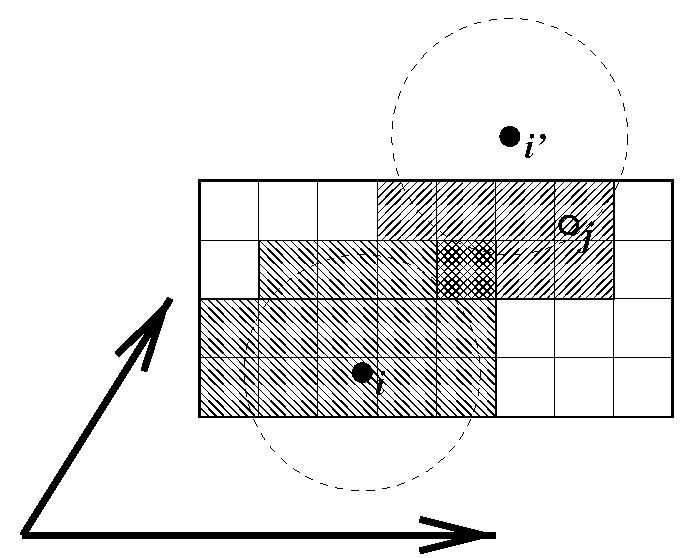
\includegraphics[width=8cm]{plots/nstric}}
\caption {Grid search in two dimensions. The arrows are the box vectors.}
\label{fig:grid}
\end{figure}

\subsubsection{Grid search\swapindexquiet{grid}{search}}
\label{sec:nsgrid}
The grid search is schematically depicted in \figref{grid}.  All
particles are put on the {\nsgrid}, with the smallest spacing $\ge$
$R_c/2$ in each of the directions.  In the direction of each box
vector, a particle $i$ has three images. For each direction the image
may be -1,0 or 1, corresponding to a translation over -1, 0 or +1 box
vector. We do not search the surrounding {\nsgrid} cells for neighbors
of $i$ and then calculate the image, but rather construct the images
first and then search neighbors corresponding to that image of $i$.
As \figref{grid} shows, some grid cells may be searched more than once
for different images of $i$. This is not a problem, since, due to the
minimum image convention, at most one image will ``see'' the
$j$-particle.  For every particle, fewer than 125 (5$^3$) neighboring
cells are searched.  Therefore, the algorithm scales linearly with the
number of particles.  Although the prefactor is large, the scaling
behavior makes the algorithm far superior over the standard $O(N^2)$
algorithm when there are more than a few hundred particles.  The
grid search is equally fast for rectangular and triclinic boxes.  Thus
for most protein and peptide simulations the rhombic dodecahedron will
be the preferred box shape.
} % Brace matches ifthenelse test for gmxlite

\ifthenelse{\equal{\gmxlite}{1}}{}{
\subsubsection{Charge groups}
\label{sec:chargegroup}\swapindexquiet{charge}{group}%
Charge groups were originally introduced to reduce cut-off artifacts
of Coulomb interactions. When a plain cut-off is used, significant
jumps in the potential and forces arise when atoms with (partial) charges
move in and out of the cut-off radius. When all chemical moieties have
a net charge of zero, these jumps can be reduced by moving groups
of atoms with net charge zero, called charge groups, in and
out of the neighbor list. This reduces the cut-off effects from
the charge-charge level to the dipole-dipole level, which decay
much faster. With the advent of full range electrostatics methods,
such as particle-mesh Ewald (\secref{pme}), the use of charge groups is
no longer required for accuracy. It might even have a slight negative effect
on the accuracy or efficiency, depending on how the neighbor list is made
and the interactions are calculated.

But there is still an important reason for using ``charge groups'': efficiency with the group cut-off scheme.
Where applicable, neighbor searching is carried out on the basis of
charge groups which are defined in the molecular topology.
If the nearest image distance between the {\em
geometrical centers} of the atoms of two charge groups is less than
the cut-off radius, all atom pairs between the charge groups are
included in the pair list.
The neighbor searching for a water system, for instance,
is $3^2=9$ times faster when each molecule is treated as a charge group.
Also the highly optimized water force loops (see \secref{waterloops})
only work when all atoms in a water molecule form a single charge group.
Currently the name {\em neighbor-search group} would be more appropriate,
but the name charge group is retained for historical reasons.
When developing a new force field, the advice is to use charge groups
of 3 to 4 atoms for optimal performance. For all-atom force fields
this is relatively easy, as one can simply put hydrogen atoms, and in some
case oxygen atoms, in the same charge group as the heavy atom they
are connected to; for example: CH$_3$, CH$_2$, CH, NH$_2$, NH, OH, CO$_2$, CO.

With the Verlet cut-off scheme, charge groups are ignored.

} % Brace matches ifthenelse test for gmxlite

\subsection{Compute forces}
\label{subsec:forces}

\subsubsection{Potential energy}
When forces are computed, the \swapindex{potential}{energy} of each
interaction term is computed as well. The total potential energy is
summed for various contributions, such as Lennard-Jones, Coulomb, and
bonded terms. It is also possible to compute these contributions for
{\em energy-monitor groups} of atoms that are separately defined (see
\secref{groupconcept}).

\subsubsection{Kinetic energy and temperature}
The \normindex{temperature} is given by the total
\swapindex{kinetic}{energy} of the $N$-particle system:
\beq
E_{kin} = \half \sum_{i=1}^N m_i v_i^2
\eeq
From this the absolute temperature $T$ can be computed using:
\beq
\half N_{\mathrm{df}} kT = E_{\mathrm{kin}}
\label{eqn:E-T}
\eeq
where $k$ is Boltzmann's constant and $N_{df}$ is the number of
degrees of freedom which can be computed from:
\beq
N_{\mathrm{df}}  ~=~     3 N - N_c - N_{\mathrm{com}}
\eeq
Here $N_c$ is the number of {\em \normindex{constraints}} imposed on the system.
When performing molecular dynamics $N_{\mathrm{com}}=3$ additional degrees of
freedom must be removed, because the three
center-of-mass velocities are constants of the motion, which are usually
set to zero. When simulating in vacuo, the rotation around the center of mass
can also be removed, in this case $N_{\mathrm{com}}=6$.
When more than one temperature-coupling group\index{temperature-coupling group} is used, the number of degrees
of freedom for group $i$ is:
\beq
N^i_{\mathrm{df}}  ~=~  (3 N^i - N^i_c) \frac{3 N - N_c - N_{\mathrm{com}}}{3 N - N_c}
\eeq

The kinetic energy can also be written as a tensor, which is necessary
for pressure calculation in a triclinic system, or systems where shear
forces  are imposed:
\beq
{\bf E}_{\mathrm{kin}} = \half \sum_i^N m_i \vvi \otimes \vvi
\eeq

\subsubsection{Pressure and virial}
The \normindex{pressure} 
tensor {\bf P} is calculated from the difference between 
kinetic energy $E_{\mathrm{kin}}$ and the \normindex{virial} ${\bf \Xi}$:
\beq
{\bf P} = \frac{2}{V} ({\bf E}_{\mathrm{kin}}-{\bf \Xi})
\label{eqn:P}
\eeq
where $V$ is the volume of the computational box. 
The scalar pressure $P$, which can be used for pressure coupling in the case
of isotropic systems, is computed as:
\beq
P       = {\rm trace}({\bf P})/3
\eeq

The virial ${\bf \Xi}$ tensor is defined as:
\beq
{\bf \Xi} = -\half \sum_{i<j} \rvij \otimes \Fvij 
\label{eqn:Xi}
\eeq

\ifthenelse{\equal{\gmxlite}{1}}{}{
The {\gromacs} implementation of the virial computation is described
in \secref{virial}.
} % Brace matches ifthenelse test for gmxlite


\subsection{The \swapindex{leap-frog}{integrator}}
\label{subsec:update}
\begin{figure}
\centerline{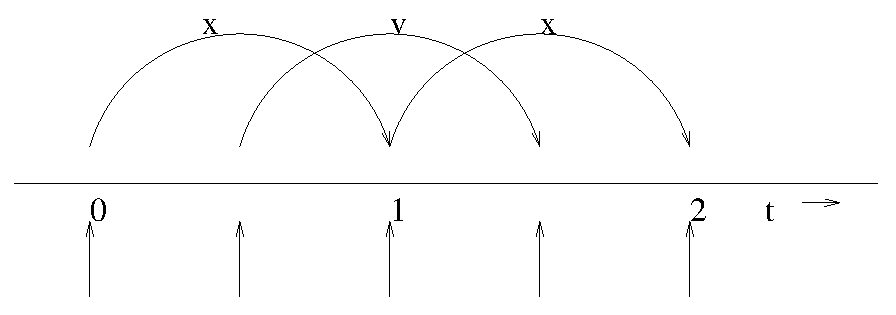
\includegraphics[width=8cm]{plots/leapfrog}}
\caption[The Leap-Frog integration method.]{The Leap-Frog integration method. The algorithm is called Leap-Frog because $\ve{r}$ and $\ve{v}$ are leaping
like  frogs over each other's backs.}
\label{fig:leapfrog}
\end{figure}

The default MD integrator in {\gromacs} is the so-called {\em leap-frog} 
algorithm~\cite{Hockney74} for the integration of the equations of
motion.  When extremely accurate integration with temperature
and/or pressure coupling is required, the velocity Verlet integrators
are also present and may be preferable (see \ssecref{vverlet}). The leap-frog
algorithm uses positions $\ve{r}$ at time $t$ and
velocities $\ve{v}$ at time $t-\hDt$; it updates positions and
velocities using the forces
$\ve{F}(t)$ determined by the positions at time $t$ using these relations:
\bea
\label{eqn:leapfrogv}
\ve{v}(t+\hDt)  &~=~&   \ve{v}(t-\hDt)+\frac{\Dt}{m}\ve{F}(t)   \\
\ve{r}(t+\Dt)   &~=~&   \ve{r}(t)+\Dt\ve{v}(t+\hDt)
\eea
The algorithm is visualized in \figref{leapfrog}.
It produces trajectories that are identical to the Verlet~\cite{Verlet67} algorithm,
whose position-update relation is
\beq
\ve{r}(t+\Dt)~=~2\ve{r}(t) - \ve{r}(t-\Dt) + \frac{1}{m}\ve{F}(t)\Dt^2+O(\Dt^4)
\eeq
The algorithm is of third order in $\ve{r}$ and is time-reversible.
See ref.~\cite{Berendsen86b} for the merits of this algorithm and comparison
with other time integration algorithms.

The \swapindex{equations of}{motion} are modified for temperature
coupling and pressure coupling, and extended to include the
conservation of constraints, all of which are described below.  

\subsection{The \swapindex{velocity Verlet}{integrator}}
\label{subsec:vverlet}
The velocity Verlet algorithm~\cite{Swope82} is also implemented in
{\gromacs}, though it is not yet fully integrated with all sets of
options.  In velocity Verlet, positions $\ve{r}$ and velocities
$\ve{v}$ at time $t$ are used to integrate the equations of motion;
velocities at the previous half step are not required.  \bea
\label{eqn:velocityverlet1}
\ve{v}(t+\hDt)  &~=~&   \ve{v}(t)+\frac{\Dt}{2m}\ve{F}(t)   \\
\ve{r}(t+\Dt)   &~=~&   \ve{r}(t)+\Dt\,\ve{v}(t+\hDt) \\
\ve{v}(t+\Dt)   &~=~&   \ve{v}(t+\hDt)+\frac{\Dt}{2m}\ve{F}(t+\Dt)
\eea
or, equivalently,
\bea
\label{eqn:velocityverlet2}
\ve{r}(t+\Dt)   &~=~&   \ve{r}(t)+ \Dt\,\ve{v} + \frac{\Dt^2}{2m}\ve{F}(t) \\
\ve{v}(t+\Dt)   &~=~&   \ve{v}(t)+ \frac{\Dt}{2m}\left[\ve{F}(t) + \ve{F}(t+\Dt)\right]
\eea
With no temperature or pressure coupling, and with {\em corresponding}
starting points, leap-frog and velocity Verlet will generate identical
trajectories, as can easily be verified by hand from the equations
above.  Given a single starting file with the {\em same} starting
point $\ve{x}(0)$ and $\ve{v}(0)$, leap-frog and velocity Verlet will
{\em not} give identical trajectories, as leap-frog will interpret the
velocities as corresponding to $t=-\hDt$, while velocity Verlet will
interpret them as corresponding to the timepoint $t=0$.

\subsection{Understanding reversible integrators: The Trotter decomposition}
To further understand the relationship between velocity Verlet and
leap-frog integration, we introduce the reversible Trotter formulation
of dynamics, which is also useful to understanding implementations of
thermostats and barostats in {\gromacs}.

A system of coupled, first-order differential equations can be evolved
from time $t = 0$ to time $t$ by applying the evolution operator
\bea
\Gamma(t) &=& \exp(iLt) \Gamma(0) \nonumber \\
iL &=& \dot{\Gamma}\cdot \nabla_{\Gamma},
\eea
where $L$ is the Liouville operator, and $\Gamma$ is the
multidimensional vector of independent variables (positions and
velocities).
A short-time approximation to the true operator, accurate at time $\Dt
= t/P$, is applied $P$ times in succession to evolve the system as
\beq
\Gamma(t) = \prod_{i=1}^P \exp(iL\Dt) \Gamma(0)
\eeq
For NVE dynamics, the Liouville operator is
\bea
iL = \sum_{i=1}^{N} \vv_i \cdot \nabla_{\rv_i} + \sum_{i=1}^N \frac{1}{m_i}\F(r_i) \cdot \nabla_{\vv_i}.
\eea
This can be split into two additive operators
\bea
iL_1 &=& \sum_{i=1}^N \frac{1}{m_i}\F(r_i) \cdot \nabla_{\vv_i} \nonumber \\
iL_2 &=& \sum_{i=1}^{N} \vv_i \cdot \nabla_{\rv_i} 
\eea
Then a short-time, symmetric, and thus reversible approximation of the true dynamics will be
\bea
\exp(iL\Dt) = \exp(iL_2\hDt) \exp(iL_1\Dt) \exp(iL_2\hDt) + \mathcal{O}(\Dt^3).
\label{eq:NVE_Trotter}
\eea
This corresponds to velocity Verlet integration.  The first
exponential term over $\hDt$ corresponds to a velocity half-step, the
second exponential term over $\Dt$ corresponds to a full velocity
step, and the last exponential term over $\hDt$ is the final velocity
half step.  For future times $t = n\Dt$, this becomes
\bea
\exp(iLn\Dt) &\approx&  \left(\exp(iL_2\hDt) \exp(iL_1\Dt) \exp(iL_2\hDt)\right)^n \nonumber \\
             &\approx&  \exp(iL_2\hDt) \bigg(\exp(iL_1\Dt) \exp(iL_2\Dt)\bigg)^{n-1} \nonumber \\
             &       &  \;\;\;\; \exp(iL_1\Dt) \exp(iL_2\hDt) 
\eea
This formalism allows us to easily see the difference between the
different flavors of Verlet integrators.  The leap-frog integrator can
be seen as starting with Eq.~\ref{eq:NVE_Trotter} with the
$\exp\left(iL_1 \dt\right)$ term, instead of the half-step velocity
term, yielding
\bea 
\exp(iLn\dt) &=& \exp\left(iL_1 \dt\right) \exp\left(iL_2 \Dt \right) + \mathcal{O}(\Dt^3).
\eea 
Here, the full step in velocity is between $t-\hDt$ and $t+\hDt$,
since it is a combination of the velocity half steps in velocity
Verlet. For future times $t = n\Dt$, this becomes
\bea 
\exp(iLn\dt) &\approx& \bigg(\exp\left(iL_1 \dt\right) \exp\left(iL_2 \Dt \right)  \bigg)^{n}.
\eea 
Although at first this does not appear symmetric, as long as the full velocity
step is between $t-\hDt$ and $t+\hDt$, then this is simply a way of
starting velocity Verlet at a different place in the cycle.

Even though the trajectory and thus potential energies are identical
between leap-frog and velocity Verlet, the kinetic energy and
temperature will not necessarily be the same.  Standard velocity
Verlet uses the velocities at the $t$ to calculate the kinetic energy
and thus the temperature only at time $t$; the kinetic energy is then a sum over all particles
\bea
KE_{\mathrm{full}}(t) &=& \sum_i \left(\frac{1}{2m_i}\ve{v}_i(t)\right)^2 \nonumber\\ 
      &=& \sum_i \frac{1}{2m_i}\left(\frac{1}{2}\ve{v}_i(t-\hDt)+\frac{1}{2}\ve{v}_i(t+\hDt)\right)^2,
\eea
with the square on the {\em outside} of the average.  Standard
leap-frog calculates the kinetic energy at time $t$ based on the
average kinetic energies at the timesteps $t+\hDt$ and $t-\hDt$, or
the sum over all particles
\bea
KE_{\mathrm{average}}(t) &=& \sum_i \frac{1}{2m_i}\left(\frac{1}{2}\ve{v}_i(t-\hDt)^2+\frac{1}{2}\ve{v}_i(t+\hDt)^2\right),
\eea
where the square is {\em inside} the average.

A non-standard variant of velocity Verlet which averages the kinetic
energies $KE(t+\hDt)$ and $KE(t-\hDt)$, exactly like leap-frog, is also
now implemented in {\gromacs} (as {\tt .mdp} file option {\tt md-vv-avek}).  Without
temperature and pressure coupling, velocity Verlet with
half-step-averaged kinetic energies and leap-frog will be identical up
to numerical precision.  For temperature- and pressure-control schemes,
however, velocity Verlet with half-step-averaged kinetic energies and
leap-frog will be different, as will be discussed in the section in
thermostats and barostats.

The half-step-averaged kinetic energy and temperature are slightly more
accurate for a given step size; the difference in average kinetic
energies using the half-step-averaged kinetic energies ({\em md} and
{\em md-vv-avek}) will be closer to the kinetic energy obtained in the
limit of small step size than will the full-step kinetic energy (using
{\em md-vv}).  For NVE simulations, this difference is usually not
significant, since the positions and velocities of the particles are
still identical; it makes a difference in the way the the temperature
of the simulations are {\em interpreted}, but {\em not} in the
trajectories that are produced.  Although the kinetic energy is more
accurate with the half-step-averaged method, meaning that it changes
less as the timestep gets large, it is also more noisy.  The RMS deviation
of the total energy of the system (sum of kinetic plus
potential) in the half-step-averaged kinetic energy case will be
higher (about twice as high in most cases) than the full-step kinetic
energy.  The drift will still be the same, however, as again, the
trajectories are identical.

For NVT simulations, however, there {\em will} be a difference, as
discussed in the section on temperature control, since the velocities
of the particles are adjusted such that kinetic energies of the
simulations, which can be calculated either way, reach the
distribution corresponding to the set temperature.  In this case, the
three methods will not give identical results.

Because the velocity and position are both defined at the same time
$t$ the velocity Verlet integrator can be used for some methods,
especially rigorously correct pressure control methods, that are not
actually possible with leap-frog.  The integration itself takes
negligibly more time than leap-frog, but twice as many communication
calls are currently required.  In most cases, and especially for large
systems where communication speed is important for parallelization and
differences between thermodynamic ensembles vanish in the $1/N$ limit,
and when only NVT ensembles are required, leap-frog will likely be the
preferred integrator.  For pressure control simulations where the fine
details of the thermodynamics are important, only velocity Verlet
allows the true ensemble to be calculated.  In either case, simulation
with double precision may be required to get fine details of
thermodynamics correct.

\subsection{Multiple time stepping}
Several other simulation packages uses multiple time stepping for
bonds and/or the PME mesh forces. In {\gromacs} we have not implemented
this (yet), since we use a different philosophy. Bonds can be constrained
(which is also a more sound approximation of a physical quantum
oscillator), which allows the smallest time step to be increased
to the larger one. This not only halves the number of force calculations,
but also the update calculations. For even larger time steps, angle vibrations
involving hydrogen atoms can be removed using virtual interaction
\ifthenelse{\equal{\gmxlite}{1}}
{sites,}
{sites (see \secref{rmfast}),}
which brings the shortest time step up to
PME mesh update frequency of a multiple time stepping scheme.

\subsection{Temperature coupling\index{temperature coupling}}
While direct use of molecular dynamics gives rise to the NVE (constant
number, constant volume, constant energy ensemble), most quantities
that we wish to calculate are actually from a constant temperature
(NVT) ensemble, also called the canonical ensemble. {\gromacs} can use
the {\em weak-coupling} scheme of Berendsen~\cite{Berendsen84},
stochastic randomization through the Andersen
thermostat~\cite{Andersen80}, the extended ensemble Nos{\'e}-Hoover
scheme~\cite{Nose84,Hoover85}, or a velocity-rescaling
scheme~\cite{Bussi2007a} to simulate constant temperature, with
advantages of each of the schemes laid out below.

There are several other reasons why it might be necessary to control
the temperature of the system (drift during equilibration, drift as a
result of force truncation and integration errors, heating due to
external or frictional forces), but this is not entirely correct to do
from a thermodynamic standpoint, and in some cases only masks the
symptoms (increase in temperature of the system) rather than the
underlying problem (deviations from correct physics in the dynamics).
For larger systems, errors in ensemble averages and structural
properties incurred by using temperature control to remove slow drifts
in temperature appear to be negligible, but no completely
comprehensive comparisons have been carried out, and some caution must
be taking in interpreting the results.

When using temperature and/or pressure coupling the total energy is
no longer conserved. Instead there is a \normindex{conserved energy quantity}
the formula of which will depend on the combination or temperature and
pressure coupling algorithm used. For all coupling algorithms, except
for Andersen temperature coupling and Parrinello-Rahman pressure coupling
combined with shear stress, the conserved energy quantity is computed
and stored in the energy and log file. Note that this quantity will not
be conserved when external forces are applied to the system, such as
pulling on group with a changing distance or an electric field.
Furthermore, how well the energy is conserved depends on the accuracy
of all algorithms involved in the simulation. Usually the algorithms that
cause most drift are constraints and the pair-list buffer, depending
on the parameters used.

\subsubsection{Berendsen temperature coupling\pawsindexquiet{Berendsen}{temperature coupling}\index{weak coupling}}
The Berendsen algorithm mimics weak coupling with first-order 
kinetics to an external heat bath with given temperature $T_0$. 
See ref.~\cite{Berendsen91} for a comparison with the
Nos{\'e}-Hoover scheme. The effect of this algorithm is
that a deviation of the system temperature from $T_0$ is slowly
corrected according to:
\beq
\frac{\de T}{\de t} = \frac{T_0-T}{\tau}
\label{eqn:Tcoupling}
\eeq
which means that a temperature deviation decays exponentially with a
time constant $\tau$.
This method of coupling has the advantage that the strength of the
coupling can be varied and adapted to the user requirement: for
equilibration purposes the coupling time can be taken quite short
({\eg} 0.01 ps), but for reliable equilibrium runs it can be taken much
longer ({\eg} 0.5 ps) in which case it hardly influences the
conservative dynamics. 

The Berendsen thermostat suppresses the fluctuations of the kinetic
energy.  This means that one does not generate a proper canonical
ensemble, so rigorously, the sampling will be incorrect.  This
error scales with $1/N$, so for very large systems most ensemble
averages will not be affected significantly, except for the
distribution of the kinetic energy itself.  However, fluctuation
properties, such as the heat capacity, will be affected.  A similar
thermostat which does produce a correct ensemble is the velocity
rescaling thermostat~\cite{Bussi2007a} described below.

The heat flow into or out of the system is affected by scaling the
velocities of each particle every step, or every $n_\mathrm{TC}$ steps,
with a time-dependent factor $\lambda$, given by:
\beq 
\lambda = \left[ 1 + \frac{n_\mathrm{TC} \Delta t}{\tau_T}
\left\{\frac{T_0}{T(t -  \hDt)} - 1 \right\} \right]^{1/2}
\label{eqn:lambda}
\eeq
The parameter $\tau_T$ is close, but not exactly equal, to the time constant
$\tau$ of the temperature coupling (\eqnref{Tcoupling}):
\beq
\tau = 2 C_V \tau_T / N_{df} k
\eeq
where $C_V$ is the total heat capacity of the system, $k$ is Boltzmann's
constant, and $N_{df}$ is the total number of degrees of freedom. The
reason that $\tau \neq \tau_T$ is that the kinetic energy change
caused by scaling the velocities is partly redistributed between
kinetic and potential energy and hence the change in temperature is
less than the scaling energy.  In practice, the ratio $\tau / \tau_T$
ranges from 1 (gas) to 2 (harmonic solid) to 3 (water). When we use
the term ``temperature coupling time constant,'' we mean the parameter
\normindex{$\tau_T$}.  
{\bf Note} that in practice the scaling factor $\lambda$ is limited to 
the range of 0.8 $<= \lambda <=$ 1.25, to avoid scaling by very large
numbers which may crash the simulation. In normal use, 
$\lambda$ will always be much closer to 1.0.

The thermostat modifies the kinetic energy at each scaling step by:
\beq
\Delta E_k = (\lambda - 1)^2 E_k
\eeq
The sum of these changes over the run needs to subtracted from the total energy
to obtain the conserved energy quantity.

\subsubsection{Velocity-rescaling temperature coupling\pawsindexquiet{velocity-rescaling}{temperature coupling}}
The velocity-rescaling thermostat~\cite{Bussi2007a} is essentially a Berendsen
thermostat (see above) with an additional stochastic term that ensures
a correct kinetic energy distribution by modifying it according to
\beq
\de K = (K_0 - K) \frac{\de t}{\tau_T} + 2 \sqrt{\frac{K K_0}{N_f}} \frac{\de W}{\sqrt{\tau_T}},
\label{eqn:vrescale}
\eeq
where $K$ is the kinetic energy, $N_f$ the number of degrees of freedom and $\de W$ a Wiener process.
There are no additional parameters, except for a random seed.
This thermostat produces a correct canonical ensemble and still has
the advantage of the Berendsen thermostat: first order decay of
temperature deviations and no oscillations.

\subsubsection{\normindex{Andersen thermostat}}
One simple way to maintain a thermostatted ensemble is to take an
$NVE$ integrator and periodically re-select the velocities of the
particles from a Maxwell-Boltzmann distribution.~\cite{Andersen80}
This can either be done by randomizing all the velocities
simultaneously (massive collision) every $\tau_T/\Dt$ steps ({\tt andersen-massive}), or by
randomizing every particle with some small probability every timestep ({\tt andersen}),
equal to $\Dt/\tau$, where in both cases $\Dt$ is the timestep and
$\tau_T$ is a characteristic coupling time scale.
Because of the way constraints operate, all particles in the same
constraint group must be randomized simultaneously.  Because of
parallelization issues, the {\tt andersen} version cannot currently (5.0) be
used in systems with constraints. {\tt andersen-massive} can be used regardless of constraints.
This thermostat is also currently only possible with velocity Verlet algorithms,
because it operates directly on the velocities at each timestep.

This algorithm completely avoids some of the ergodicity issues of other thermostatting
algorithms, as energy cannot flow back and forth between energetically
decoupled components of the system as in velocity scaling motions.
However, it can slow down the kinetics of system by randomizing
correlated motions of the system, including slowing sampling when
$\tau_T$ is at moderate levels (less than 10 ps). This algorithm
should therefore generally not be used when examining kinetics or
transport properties of the system.~\cite{Basconi2013}

% \ifthenelse{\equal{\gmxlite}{1}}{}{
\subsubsection{Nos{\'e}-Hoover temperature coupling\index{Nose-Hoover temperature coupling@Nos{\'e}-Hoover temperature coupling|see{temperature coupling, Nos{\'e}-Hoover}}{\index{temperature coupling Nose-Hoover@temperature coupling Nos{\'e}-Hoover}}\index{extended ensemble}}

The Berendsen weak-coupling algorithm is
extremely efficient for relaxing a system to the target temperature,
but once the system has reached equilibrium it might be more
important to probe a correct canonical ensemble. This is unfortunately
not the case for the weak-coupling scheme.

To enable canonical ensemble simulations, {\gromacs} also supports the
extended-ensemble approach first proposed by Nos{\'e}~\cite{Nose84}
and later modified by Hoover~\cite{Hoover85}. The system Hamiltonian is
extended by introducing a thermal reservoir and a friction term in the
equations of motion.  The friction force is proportional to the
product of each particle's velocity and a friction parameter, $\xi$.
This friction parameter (or ``heat bath'' variable) is a fully
dynamic quantity with its own momentum ($p_{\xi}$) and equation of
motion; the time derivative is calculated from the difference between
the current kinetic energy and the reference temperature.  

In this formulation, the particles' equations of motion in
\figref{global} are replaced by:
\beq
\frac {\de^2\ve{r}_i}{\de t^2} = \frac{\ve{F}_i}{m_i} - 
\frac{p_{\xi}}{Q}\frac{\de \ve{r}_i}{\de t} ,
\label{eqn:NH-eqn-of-motion}
\eeq where the equation of motion for the heat bath parameter $\xi$ is:
\beq \frac {\de p_{\xi}}{\de t} = \left( T - T_0 \right).  \eeq The
reference temperature is denoted $T_0$, while $T$ is the current
instantaneous temperature of the system. The strength of the coupling
is determined by the constant $Q$ (usually called the ``mass parameter''
of the reservoir) in combination with the reference
temperature.~\footnote{Note that some derivations, an alternative
  notation $\xi_{\mathrm{alt}} = v_{\xi} = p_{\xi}/Q$ is used.}

The conserved quantity for the Nos{\'e}-Hoover equations of motion is not 
the total energy, but rather
\bea
H = \sum_{i=1}^{N} \frac{\pb_i}{2m_i} + U\left(\rv_1,\rv_2,\ldots,\rv_N\right) +\frac{p_{\xi}^2}{2Q} + N_fkT\xi,
\eea
where $N_f$ is the total number of degrees of freedom.

In our opinion, the mass parameter is a somewhat awkward way of
describing coupling strength, especially due to its dependence on
reference temperature (and some implementations even include the
number of degrees of freedom in your system when defining $Q$).  To
maintain the coupling strength, one would have to change $Q$ in
proportion to the change in reference temperature. For this reason, we
prefer to let the {\gromacs} user work instead with the period
$\tau_T$ of the oscillations of kinetic energy between the system and
the reservoir instead. It is directly related to $Q$ and $T_0$ via:
\beq
Q = \frac {\tau_T^2 T_0}{4 \pi^2}.
\eeq
This provides a much more intuitive way of selecting the
Nos{\'e}-Hoover coupling strength (similar to the weak-coupling
relaxation), and in addition $\tau_T$ is independent of system size
and reference temperature.

It is however important to keep the difference between the 
weak-coupling scheme and the Nos{\'e}-Hoover algorithm in mind: 
Using weak coupling you get a
strongly damped {\em exponential relaxation}, 
while the Nos{\'e}-Hoover approach
produces an {\em oscillatory relaxation}. 
The actual time it takes to relax with Nos{\'e}-Hoover coupling is 
several times larger than the period of the
oscillations that you select. These oscillations (in contrast
to exponential relaxation) also means that
the time constant normally should be 4--5 times larger
than the relaxation time used with weak coupling, but your 
mileage may vary.

Nos{\'e}-Hoover dynamics in simple systems such as collections of
harmonic oscillators, can be {\em nonergodic}, meaning that only a
subsection of phase space is ever sampled, even if the simulations
were to run for infinitely long.  For this reason, the Nos{\'e}-Hoover
chain approach was developed, where each of the Nos{\'e}-Hoover
thermostats has its own Nos{\'e}-Hoover thermostat controlling its
temperature.  In the limit of an infinite chain of thermostats, the
dynamics are guaranteed to be ergodic. Using just a few chains can
greatly improve the ergodicity, but recent research has shown that the
system will still be nonergodic, and it is still not entirely clear
what the practical effect of this~\cite{Cooke2008}. Currently, the
default number of chains is 10, but this can be controlled by the
user.  In the case of chains, the equations are modified in the
following way to include a chain of thermostatting
particles~\cite{Martyna1992}:

\bea
\frac {\de^2\ve{r}_i}{\de t^2} &~=~& \frac{\ve{F}_i}{m_i} - \frac{p_{{\xi}_1}}{Q_1} \frac{\de \ve{r}_i}{\de t} \nonumber \\
\frac {\de p_{{\xi}_1}}{\de t} &~=~& \left( T - T_0 \right) - p_{{\xi}_1} \frac{p_{{\xi}_2}}{Q_2} \nonumber \\
\frac {\de p_{{\xi}_{i=2\ldots N}}}{\de t} &~=~& \left(\frac{p_{\xi_{i-1}}^2}{Q_{i-1}} -kT\right) - p_{\xi_i} \frac{p_{\xi_{i+1}}}{Q_{i+1}} \nonumber \\
\frac {\de p_{\xi_N}}{\de t} &~=~& \left(\frac{p_{\xi_{N-1}}^2}{Q_{N-1}}-kT\right)
\label{eqn:NH-chain-eqn-of-motion}
\eea
The conserved quantity for Nos{\'e}-Hoover chains is
\bea
H = \sum_{i=1}^{N} \frac{\pb_i}{2m_i} + U\left(\rv_1,\rv_2,\ldots,\rv_N\right) +\sum_{k=1}^M\frac{p^2_{\xi_k}}{2Q^{\prime}_k} + N_fkT\xi_1 + kT\sum_{k=2}^M \xi_k 
\eea
The values and velocities of the Nos{\'e}-Hoover thermostat variables
are generally not included in the output, as they take up a fair
amount of space and are generally not important for analysis of
simulations, but this can be overridden by defining the environment
variable {\tt GMX_NOSEHOOVER_CHAINS}, which will print the values of all
the positions and velocities of all Nos{\'e}-Hoover particles in the
chain to the {\tt .edr} file.  Leap-frog simulations currently can only have 
Nos{\'e}-Hoover chain lengths of 1, but this will likely be updated in 
later version.

As described in the integrator section, for temperature coupling, the
temperature that the algorithm attempts to match to the reference
temperature is calculated differently in velocity Verlet and leap-frog
dynamics.  Velocity Verlet ({\em md-vv}) uses the full-step kinetic
energy, while leap-frog and {\em md-vv-avek} use the half-step-averaged
kinetic energy.

We can examine the Trotter decomposition again to better understand
the differences between these constant-temperature integrators.  In
the case of Nos{\'e}-Hoover dynamics (for simplicity, using a chain
with $N=1$, with more details in Ref.~\cite{Martyna1996}), we split
the Liouville operator as
\beq
iL = iL_1 + iL_2 + iL_{\mathrm{NHC}},
\eeq
where
\bea
iL_1 &=& \sum_{i=1}^N \left[\frac{\pb_i}{m_i}\right]\cdot \frac{\partial}{\partial \rv_i} \nonumber \\
iL_2 &=& \sum_{i=1}^N \F_i\cdot \frac{\partial}{\partial \pb_i} \nonumber \\
iL_{\mathrm{NHC}} &=& \sum_{i=1}^N-\frac{p_{\xi}}{Q}\vv_i\cdot \nabla_{\vv_i} +\frac{p_{\xi}}{Q}\frac{\partial }{\partial \xi} + \left( T - T_0 \right)\frac{\partial }{\partial p_{\xi}}
\eea
For standard velocity Verlet with Nos{\'e}-Hoover temperature control, this becomes
\bea  
\exp(iL\dt) &=& \exp\left(iL_{\mathrm{NHC}}\dt/2\right) \exp\left(iL_2 \dt/2\right) \nonumber \\
&&\exp\left(iL_1 \dt\right) \exp\left(iL_2 \dt/2\right) \exp\left(iL_{\mathrm{NHC}}\dt/2\right) + \mathcal{O}(\Dt^3).
\eea
For half-step-averaged temperature control using {\em md-vv-avek},
this decomposition will not work, since we do not have the full step
temperature until after the second velocity step.  However, we can
construct an alternate decomposition that is still reversible, by
switching the place of the NHC and velocity portions of the
decomposition:
\bea  
\exp(iL\dt) &=& \exp\left(iL_2 \dt/2\right) \exp\left(iL_{\mathrm{NHC}}\dt/2\right)\exp\left(iL_1 \dt\right)\nonumber \\
&&\exp\left(iL_{\mathrm{NHC}}\dt/2\right) \exp\left(iL_2 \dt/2\right)+ \mathcal{O}(\Dt^3)
\label{eq:half_step_NHC_integrator}
\eea
This formalism allows us to easily see the difference between the
different flavors of velocity Verlet integrator.  The leap-frog
integrator can be seen as starting with
Eq.~\ref{eq:half_step_NHC_integrator} just before the $\exp\left(iL_1
\dt\right)$ term, yielding:
\bea  
\exp(iL\dt) &=&  \exp\left(iL_1 \dt\right) \exp\left(iL_{\mathrm{NHC}}\dt/2\right) \nonumber \\
&&\exp\left(iL_2 \dt\right) \exp\left(iL_{\mathrm{NHC}}\dt/2\right) + \mathcal{O}(\Dt^3)
\eea
and then using some algebra tricks to solve for some quantities are
required before they are actually calculated~\cite{Holian95}.

% }

\subsubsection{Group temperature coupling}\index{temperature-coupling group}%
In {\gromacs} temperature coupling can be performed on groups of
atoms, typically a protein and solvent. The reason such algorithms
were introduced is that energy exchange between different components
is not perfect, due to different effects including cut-offs etc. If
now the whole system is coupled to one heat bath, water (which
experiences the largest cut-off noise) will tend to heat up and the
protein will cool down. Typically 100 K differences can be obtained.
With the use of proper electrostatic methods (PME) these difference
are much smaller but still not negligible.  The parameters for
temperature coupling in groups are given in the {\tt mdp} file.
Recent investigation has shown that small temperature differences
between protein and water may actually be an artifact of the way
temperature is calculated when there are finite timesteps, and very
large differences in temperature are likely a sign of something else
seriously going wrong with the system, and should be investigated
carefully~\cite{Eastwood2010}.

One special case should be mentioned: it is possible to temperature-couple only
part of the system, leaving other parts without temperature
coupling. This is done by specifying ${-1}$ for the time constant
$\tau_T$ for the group that should not be thermostatted.  If only
part of the system is thermostatted, the system will still eventually
converge to an NVT system.  In fact, one suggestion for minimizing
errors in the temperature caused by discretized timesteps is that if
constraints on the water are used, then only the water degrees of
freedom should be thermostatted, not protein degrees of freedom, as
the higher frequency modes in the protein can cause larger deviations
from the ``true'' temperature, the temperature obtained with small
timesteps~\cite{Eastwood2010}.

\subsection{Pressure coupling\index{pressure coupling}}
In the same spirit as the temperature coupling, the system can also be
coupled to a ``pressure bath.'' {\gromacs} supports both the Berendsen
algorithm~\cite{Berendsen84} that scales coordinates and box vectors
every step, the extended-ensemble Parrinello-Rahman approach~\cite{Parrinello81,Nose83}, and for
the velocity Verlet variants, the Martyna-Tuckerman-Tobias-Klein
(MTTK) implementation of pressure
control~\cite{Martyna1996}. Parrinello-Rahman and Berendsen can be
combined with any of the temperature coupling methods above. MTTK can
only be used with Nos{\'e}-Hoover temperature control. From 5.1 afterwards,
it can only used when the system does not have constraints.

\subsubsection{Berendsen pressure coupling\pawsindexquiet{Berendsen}{pressure coupling}\index{weak coupling}}
\label{sec:berendsen_pressure_coupling}
The Berendsen algorithm rescales the 
coordinates and box vectors every step, or every $n_\mathrm{PC}$ steps,
 with a matrix {\boldmath $\mu$},
which has the effect of a first-order kinetic relaxation of the pressure
towards a given reference pressure ${\bf P}_0$ according to
\beq
\frac{\de {\bf P}}{\de t} = \frac{{\bf P}_0-{\bf P}}{\tau_p}.
\eeq
The scaling matrix {\boldmath $\mu$} is given by
\beq
\mu_{ij}
= \delta_{ij} - \frac{n_\mathrm{PC}\Delta t}{3\, \tau_p} \beta_{ij} \{P_{0ij} - P_{ij}(t) \}.
\label{eqn:mu}
\eeq
\index{isothermal compressibility}
\index{compressibility}
Here, {\boldmath $\beta$} is the isothermal compressibility of the system.
In most cases this will be a diagonal matrix, with equal elements on the
diagonal, the value of which is generally not known.
It suffices to take a rough estimate because the value of {\boldmath $\beta$}
only influences the non-critical time constant of the
pressure relaxation without affecting the average pressure itself.
For water at 1 atm and 300 K 
$\beta = 4.6 \times 10^{-10}$ Pa$^{-1} = 4.6 \times 10^{-5}$ bar$^{-1}$,
which is $7.6 \times 10^{-4}$ MD units (see \chref{defunits}).
Most other liquids have similar values.
When scaling completely anisotropically, the system has to be rotated in
order to obey \eqnref{box_rot}.
This rotation is approximated in first order in the scaling, which is usually
less than $10^{-4}$. The actual scaling matrix {\boldmath $\mu'$} is
\beq
\mbox{\boldmath $\mu'$} = 
\left(\begin{array}{ccc}
\mu_{xx} & \mu_{xy} + \mu_{yx} & \mu_{xz} + \mu_{zx} \\
0        & \mu_{yy}            & \mu_{yz} + \mu_{zy} \\
0        & 0                   & \mu_{zz}
\end{array}\right).
\eeq
The velocities are neither scaled nor rotated.
Since the equations of motion are modified by pressure coupling, the conserved
energy quantity also needs to be modified. For first order pressure coupling,
the work the barostat applies to the system every step needs to
be subtracted from the total energy to obtain the conserved energy quantity:
\beq
- \sum_{i,j} (\mu_{ij} -\delta_{ij}) P_{ij} V =
\sum_{i,j} 2(\mu_{ij} -\delta_{ij}) \Xi_{ij}
\eeq
where $\delta_{ij}$ is the Kronecker delta and  ${\bf \Xi}$ is the virial.
Note that the factor 2 originates from the factor $\frac{1}{2}$
in the virial definition (\eqnref{Xi}).


In {\gromacs}, the Berendsen scaling can also be done isotropically, 
which means that instead of $\ve{P}$ a diagonal matrix with elements of size
trace$(\ve{P})/3$ is used. For systems with interfaces, semi-isotropic 
scaling can be useful.
In this case, the $x/y$-directions are scaled isotropically and the $z$
direction is scaled independently. The compressibility in the $x/y$ or
$z$-direction can be set to zero, to scale only in the other direction(s).

If you allow full anisotropic deformations and use constraints you
might have to scale more slowly or decrease your timestep to avoid
errors from the constraint algorithms.  It is important to note that
although the Berendsen pressure control algorithm yields a simulation
with the correct average pressure, it does not yield the exact NPT
ensemble, and it is not yet clear exactly what errors this approximation
may yield.

% \ifthenelse{\equal{\gmxlite}{1}}{}{
\subsubsection{Parrinello-Rahman pressure coupling\pawsindexquiet{Parrinello-Rahman}{pressure coupling}}

In cases where the fluctuations in pressure or volume are important
{\em per se} ({\eg} to calculate thermodynamic properties), especially
for small systems, it may be a problem that the exact ensemble is not
well defined for the weak-coupling scheme, and that it does not
simulate the true NPT ensemble.

{\gromacs} also supports constant-pressure simulations using the
Parrinello-Rahman approach~\cite{Parrinello81,Nose83}, which is similar
to the Nos{\'e}-Hoover temperature coupling, and in theory gives the
true NPT ensemble.  With the Parrinello-Rahman barostat, the box
vectors as represented by the matrix \ve{b} obey the matrix equation
of motion\footnote{The box matrix representation \ve{b} in {\gromacs}
corresponds to the transpose of the box matrix representation \ve{h}
in the paper by Nos{\'e} and Klein. Because of this, some of our
equations will look slightly different.}
\beq
\frac{\de \ve{b}^2}{\de t^2}= V \ve{W}^{-1} \ve{b}'^{-1} \left( \ve{P} - \ve{P}_{ref}\right).
\eeq

The volume of the box is denoted $V$, and $\ve{W}$ is a matrix parameter that determines
the strength of the coupling. The matrices \ve{P} and \ve{P}$_{ref}$ are the 
current and reference pressures, respectively.

The equations of motion for the particles are also changed, just as
for the Nos{\'e}-Hoover coupling. In most cases you would combine the 
Parrinello-Rahman barostat with the Nos{\'e}-Hoover
thermostat, but to keep it simple we only show the Parrinello-Rahman 
modification here. The modified Hamiltonian, which will be conserved, is:
\beq
E_\mathrm{pot} + E_\mathrm{kin} +  \sum_i P_{ii} V +
\sum_{i,j} \frac{1}{2} W_{ij}  \left( \frac{\de b_{ij}}{\de t} \right)^2
\eeq
The equations of motion for the atoms, obtained from the Hamiltonian are:
\bea \frac {\de^2\ve{r}_i}{\de t^2} & = & \frac{\ve{F}_i}{m_i} -
\ve{M} \frac{\de \ve{r}_i}{\de t} , \\ \ve{M} & = & \ve{b}^{-1} \left[
  \ve{b} \frac{\de \ve{b}'}{\de t} + \frac{\de \ve{b}}{\de t} \ve{b}'
  \right] \ve{b}'^{-1}.  \eea The (inverse) mass parameter matrix
$\ve{W}^{-1}$ determines the strength of the coupling, and how the box
can be deformed.  The box restriction (\ref{eqn:box_rot}) will be
fulfilled automatically if the corresponding elements of $\ve{W}^{-1}$
are zero. Since the coupling strength also depends on the size of your
box, we prefer to calculate it automatically in {\gromacs}.  You only
have to provide the approximate isothermal compressibilities
{\boldmath $\beta$} and the pressure time constant $\tau_p$ in the
input file ($L$ is the largest box matrix element): \beq \left(
\ve{W}^{-1} \right)_{ij} = \frac{4 \pi^2 \beta_{ij}}{3 \tau_p^2 L}.
\eeq Just as for the Nos{\'e}-Hoover thermostat, you should realize
that the Parrinello-Rahman time constant is {\em not} equivalent to
the relaxation time used in the Berendsen pressure coupling algorithm.
In most cases you will need to use a 4--5 times larger time constant
with Parrinello-Rahman coupling. If your pressure is very far from
equilibrium, the Parrinello-Rahman coupling may result in very large
box oscillations that could even crash your run.  In that case you
would have to increase the time constant, or (better) use the weak-coupling
scheme to reach the target pressure, and then switch to
Parrinello-Rahman coupling once the system is in equilibrium.
Additionally, using the leap-frog algorithm, the pressure at time $t$
is not available until after the time step has completed, and so the
pressure from the previous step must be used, which makes the algorithm
not directly reversible, and may not be appropriate for high precision
thermodynamic calculations.

\subsubsection{Surface-tension coupling\pawsindexquiet{surface-tension}{pressure coupling}}
When a periodic system consists of more than one phase, separated by
surfaces which are parallel to the $xy$-plane,
the surface tension and the $z$-component of the pressure can be coupled
to a pressure bath. Presently, this only works with the Berendsen
pressure coupling algorithm in {\gromacs}.
The average surface tension $\gamma(t)$ can be calculated from
the difference between the normal and the lateral pressure
\bea
\gamma(t) & = & 
\frac{1}{n} \int_0^{L_z}
\left\{ P_{zz}(z,t) - \frac{P_{xx}(z,t) + P_{yy}(z,t)}{2} \right\} \mbox{d}z \\
& = &
\frac{L_z}{n} \left\{ P_{zz}(t) - \frac{P_{xx}(t) + P_{yy}(t)}{2} \right\},
\eea
where $L_z$ is the height of the box and $n$ is the number of surfaces.
The pressure in the z-direction is corrected by scaling the height of
the box with $\mu_{zz}$
\beq
\Delta P_{zz} = \frac{\Delta t}{\tau_p} \{ P_{0zz} - P_{zz}(t) \}
\eeq
\beq
\mu_{zz} = 1 + \beta_{zz} \Delta P_{zz}
\eeq
This is similar to normal pressure coupling, except that the factor
of $1/3$ is missing. 
The pressure correction in the $z$-direction is then used to get the
correct convergence for the surface tension to the reference value $\gamma_0$.
The correction factor for the box length in the $x$/$y$-direction is
\beq
\mu_{x/y} = 1 + \frac{\Delta t}{2\,\tau_p} \beta_{x/y}
        \left( \frac{n \gamma_0}{\mu_{zz} L_z}
        - \left\{ P_{zz}(t)+\Delta P_{zz} - \frac{P_{xx}(t) + P_{yy}(t)}{2} \right\} 
        \right)
\eeq
The value of $\beta_{zz}$ is more critical than with normal pressure
coupling. Normally an incorrect compressibility will just scale $\tau_p$,
but with surface tension coupling it affects the convergence of the surface
tension. 
When $\beta_{zz}$ is set to zero (constant box height), $\Delta P_{zz}$ is also set
to zero, which is necessary for obtaining the correct surface tension. 

\subsubsection{MTTK pressure control algorithms}

As mentioned in the previous section, one weakness of leap-frog
integration is in constant pressure simulations, since the pressure
requires a calculation of both the virial and the kinetic energy at
the full time step; for leap-frog, this information is not available
until {\em after} the full timestep.  Velocity Verlet does allow the
calculation, at the cost of an extra round of global communication,
and can compute, mod any integration errors, the true NPT ensemble.

The full equations, combining both pressure coupling and temperature
coupling, are taken from Martyna {\em et al.}~\cite{Martyna1996} and
Tuckerman~\cite{Tuckerman2006} and are referred to here as MTTK
equations (Martyna-Tuckerman-Tobias-Klein).  We introduce for
convenience $\epsilon = (1/3)\ln (V/V_0)$, where $V_0$ is a reference
volume.  The momentum of $\epsilon$ is $\veps = p_{\epsilon}/W =
\dot{\epsilon} = \dot{V}/3V$, and define $\alpha = 1 + 3/N_{dof}$ (see
Ref~\cite{Tuckerman2006})

The isobaric equations are
\bea
\dot{\rv}_i &=& \frac{\pb_i}{m_i} + \frac{\peps}{W} \rv_i \nonumber \\
\frac{\dot{\pb}_i}{m_i} &=& \frac{1}{m_i}\F_i - \alpha\frac{\peps}{W} \frac{\pb_i}{m_i} \nonumber \\
\dot{\epsilon} &=& \frac{\peps}{W} \nonumber \\
\frac{\dot{\peps}}{W} &=& \frac{3V}{W}(P_{\mathrm{int}} - P) + (\alpha-1)\left(\sum_{n=1}^N\frac{\pb_i^2}{m_i}\right),\\
\eea
where
\bea
P_{\mathrm{int}} &=& P_{\mathrm{kin}} -P_{\mathrm{vir}} = \frac{1}{3V}\left[\sum_{i=1}^N \left(\frac{\pb_i^2}{2m_i} - \rv_i \cdot \F_i\
\right)\right].
\eea
The terms including $\alpha$ are required to make phase space
incompressible~\cite{Tuckerman2006}. The $\epsilon$ acceleration term
can be rewritten as
\bea
\frac{\dot{\peps}}{W} &=& \frac{3V}{W}\left(\alpha P_{\mathrm{kin}} - P_{\mathrm{vir}} - P\right)
\eea
In terms of velocities, these equations become
\bea
\dot{\rv}_i &=& \vv_i + \veps \rv_i \nonumber \\
\dot{\vv}_i &=& \frac{1}{m_i}\F_i - \alpha\veps \vv_i \nonumber \\
\dot{\epsilon} &=& \veps \nonumber \\
\dot{\veps} &=& \frac{3V}{W}(P_{\mathrm{int}} - P) + (\alpha-1)\left( \sum_{n=1}^N \frac{1}{2} m_i \vv_i^2\right)\nonumber \\
P_{\mathrm{int}} &=& P_{\mathrm{kin}} - P_{\mathrm{vir}} = \frac{1}{3V}\left[\sum_{i=1}^N \left(\frac{1}{2} m_i\vv_i^2 - \rv_i \cdot \F_i\right)\right]
\eea
For these equations, the conserved quantity is
\bea
H = \sum_{i=1}^{N} \frac{\pb_i^2}{2m_i} + U\left(\rv_1,\rv_2,\ldots,\rv_N\right) + \frac{p_\epsilon}{2W} + PV
\eea
The next step is to add temperature control.  Adding Nos{\'e}-Hoover
chains, including to the barostat degree of freedom, where we use
$\eta$ for the barostat Nos{\'e}-Hoover variables, and $Q^{\prime}$
for the coupling constants of the thermostats of the barostats, we get
\bea
\dot{\rv}_i &=& \frac{\pb_i}{m_i} + \frac{\peps}{W} \rv_i \nonumber \\
\frac{\dot{\pb}_i}{m_i} &=& \frac{1}{m_i}\F_i - \alpha\frac{\peps}{W} \frac{\pb_i}{m_i} - \frac{p_{\xi_1}}{Q_1}\frac{\pb_i}{m_i}\nonumber \\
\dot{\epsilon} &=& \frac{\peps}{W} \nonumber \\
\frac{\dot{\peps}}{W} &=& \frac{3V}{W}(\alpha P_{\mathrm{kin}} - P_{\mathrm{vir}} - P) -\frac{p_{\eta_1}}{Q^{\prime}_1}\peps \nonumber \\
\dot{\xi}_k &=& \frac{p_{\xi_k}}{Q_k} \nonumber \\ 
\dot{\eta}_k &=& \frac{p_{\eta_k}}{Q^{\prime}_k} \nonumber \\
\dot{p}_{\xi_k} &=& G_k - \frac{p_{\xi_{k+1}}}{Q_{k+1}} \;\;\;\; k=1,\ldots, M-1 \nonumber \\ 
\dot{p}_{\eta_k} &=& G^\prime_k - \frac{p_{\eta_{k+1}}}{Q^\prime_{k+1}} \;\;\;\; k=1,\ldots, M-1 \nonumber \\
\dot{p}_{\xi_M} &=& G_M \nonumber \\
\dot{p}_{\eta_M} &=& G^\prime_M, \nonumber \\
\eea
where
\bea
P_{\mathrm{int}} &=& P_{\mathrm{kin}} - P_{\mathrm{vir}} = \frac{1}{3V}\left[\sum_{i=1}^N \left(\frac{\pb_i^2}{2m_i} - \rv_i \cdot \F_i\right)\right] \nonumber \\
G_1  &=& \sum_{i=1}^N \frac{\pb^2_i}{m_i} - N_f kT \nonumber \\
G_k  &=&  \frac{p^2_{\xi_{k-1}}}{2Q_{k-1}} - kT \;\; k = 2,\ldots,M \nonumber \\
G^\prime_1 &=& \frac{\peps^2}{2W} - kT \nonumber \\
G^\prime_k &=& \frac{p^2_{\eta_{k-1}}}{2Q^\prime_{k-1}} - kT \;\; k = 2,\ldots,M
\eea
The conserved quantity is now
\bea
H = \sum_{i=1}^{N} \frac{\pb_i}{2m_i} + U\left(\rv_1,\rv_2,\ldots,\rv_N\right) + \frac{p^2_\epsilon}{2W} + PV + \nonumber \\
\sum_{k=1}^M\frac{p^2_{\xi_k}}{2Q_k} +\sum_{k=1}^M\frac{p^2_{\eta_k}}{2Q^{\prime}_k} + N_fkT\xi_1 +  kT\sum_{i=2}^M \xi_k + kT\sum_{k=1}^M \eta_k
\eea
Returning to the Trotter decomposition formalism, for pressure control and temperature control~\cite{Martyna1996} we get:
\bea
iL = iL_1 + iL_2 + iL_{\epsilon,1} + iL_{\epsilon,2} + iL_{\mathrm{NHC-baro}} + iL_{\mathrm{NHC}}
\eea
where ``NHC-baro'' corresponds to the Nos{\`e}-Hoover chain of the barostat,
and NHC corresponds to the NHC of the particles,
\bea
iL_1 &=& \sum_{i=1}^N \left[\frac{\pb_i}{m_i} + \frac{\peps}{W}\rv_i\right]\cdot \frac{\partial}{\partial \rv_i} \\
iL_2 &=& \sum_{i=1}^N \F_i - \alpha \frac{\peps}{W}\pb_i \cdot \frac{\partial}{\partial \pb_i} \\
iL_{\epsilon,1} &=& \frac{p_\epsilon}{W} \frac{\partial}{\partial \epsilon}\\
iL_{\epsilon,2} &=& G_{\epsilon} \frac{\partial}{\partial p_\epsilon}
\eea
and where
\bea
G_{\epsilon} = 3V\left(\alpha P_{\mathrm{kin}} - P_{\mathrm{vir}} - P\right)
\eea 
Using the Trotter decomposition, we get
\bea  
\exp(iL\dt) &=& \exp\left(iL_{\mathrm{NHC-baro}}\dt/2\right)\exp\left(iL_{\mathrm{NHC}}\dt/2\right) \nonumber \nonumber \\
&&\exp\left(iL_{\epsilon,2}\dt/2\right) \exp\left(iL_2 \dt/2\right) \nonumber \nonumber \\
&&\exp\left(iL_{\epsilon,1}\dt\right) \exp\left(iL_1 \dt\right) \nonumber \nonumber \\
&&\exp\left(iL_2 \dt/2\right) \exp\left(iL_{\epsilon,2}\dt/2\right) \nonumber \nonumber \\
&&\exp\left(iL_{\mathrm{NHC}}\dt/2\right)\exp\left(iL_{\mathrm{NHC-baro}}\dt/2\right) + \mathcal{O}(\dt^3)
\eea
The action of $\exp\left(iL_1 \dt\right)$ comes from the solution of
the the differential equation 
$\dot{\rv}_i = \vv_i + \veps \rv_i$
with $\vv_i = \pb_i/m_i$ and $\veps$ constant with initial condition
$\rv_i(0)$, evaluate at $t=\Delta t$.  This yields the evolution
\beq
\rv_i(\dt) = \rv_i(0)e^{\veps \dt} + \Delta t \vv_i(0) e^{\veps \dt/2} \sinhx{\veps \dt/2}.
\eeq
The action of $\exp\left(iL_2 \dt/2\right)$ comes from the solution
of the differential equation $\dot{\vv}_i = \frac{\F_i}{m_i} -
\alpha\veps\vv_i$, yielding
\beq
\vv_i(\dt/2) = \vv_i(0)e^{-\alpha\veps \dt/2} + \frac{\Delta t}{2m_i}\F_i(0) e^{-\alpha\veps \dt/4}\sinhx{\alpha\veps \dt/4}.
\eeq
{\em md-vv-avek} uses the full step kinetic energies for determining the pressure with the pressure control,
but the half-step-averaged kinetic energy for the temperatures, which can be written as a Trotter decomposition as
\bea  
\exp(iL\dt) &=& \exp\left(iL_{\mathrm{NHC-baro}}\dt/2\right)\nonumber \exp\left(iL_{\epsilon,2}\dt/2\right) \exp\left(iL_2 \dt/2\right) \nonumber \\
&&\exp\left(iL_{\mathrm{NHC}}\dt/2\right) \exp\left(iL_{\epsilon,1}\dt\right) \exp\left(iL_1 \dt\right) \exp\left(iL_{\mathrm{NHC}}\dt/2\right) \nonumber \\
&&\exp\left(iL_2 \dt/2\right) \exp\left(iL_{\epsilon,2}\dt/2\right) \exp\left(iL_{\mathrm{NHC-baro}}\dt/2\right) + \mathcal{O}(\dt^3)
\eea

With constraints, the equations become significantly more complicated,
in that each of these equations need to be solved iteratively for the
constraint forces. Before {\gromacs} 5.1, these iterative
constraints were solved as described in~\cite{Yu2010}. From {\gromacs}
5.1 onward, MTTK with constraints has been removed because of
numerical stability issues with the iterations.

\subsubsection{Infrequent evaluation of temperature and pressure coupling}

Temperature and pressure control require global communication to
compute the kinetic energy and virial, which can become costly if
performed every step for large systems.  We can rearrange the Trotter
decomposition to give alternate symplectic, reversible integrator with
the coupling steps every $n$ steps instead of every steps.  These new
integrators will diverge if the coupling time step is too large, as
the auxiliary variable integrations will not converge.  However, in
most cases, long coupling times are more appropriate, as they disturb
the dynamics less~\cite{Martyna1996}.

Standard velocity Verlet with Nos{\'e}-Hoover temperature control has a Trotter expansion
\bea  
\exp(iL\dt) &\approx& \exp\left(iL_{\mathrm{NHC}}\dt/2\right) \exp\left(iL_2 \dt/2\right) \nonumber \\
&&\exp\left(iL_1 \dt\right) \exp\left(iL_2 \dt/2\right) \exp\left(iL_{\mathrm{NHC}}\dt/2\right).
\eea
If the Nos{\'e}-Hoover chain is sufficiently slow with respect to the motions of the system, we can
write an alternate integrator over $n$ steps for velocity Verlet as
\bea  
\exp(iL\dt) &\approx& (\exp\left(iL_{\mathrm{NHC}}(n\dt/2)\right)\left[\exp\left(iL_2 \dt/2\right)\right. \nonumber \\
&&\left.\exp\left(iL_1 \dt\right) \exp\left(iL_2 \dt/2\right)\right]^n \exp\left(iL_{\mathrm{NHC}}(n\dt/2)\right).
\eea
For pressure control, this becomes
\bea  
\exp(iL\dt) &\approx& \exp\left(iL_{\mathrm{NHC-baro}}(n\dt/2)\right)\exp\left(iL_{\mathrm{NHC}}(n\dt/2)\right) \nonumber \nonumber \\
&&\exp\left(iL_{\epsilon,2}(n\dt/2)\right) \left[\exp\left(iL_2 \dt/2\right)\right. \nonumber \nonumber \\
&&\exp\left(iL_{\epsilon,1}\dt\right) \exp\left(iL_1 \dt\right) \nonumber \nonumber \\
&&\left.\exp\left(iL_2 \dt/2\right)\right]^n \exp\left(iL_{\epsilon,2}(n\dt/2)\right) \nonumber \nonumber \\
&&\exp\left(iL_{\mathrm{NHC}}(n\dt/2)\right)\exp\left(iL_{\mathrm{NHC-baro}}(n\dt/2)\right),
\eea
where the box volume integration occurs every step, but the auxiliary variable
integrations happen every $n$ steps.

% } % Brace matches ifthenelse test for gmxlite


\subsection{The complete update algorithm}
\begin{figure}
\begin{center}
\addtolength{\fboxsep}{0.5cm}
\begin{shadowenv}[12cm]
{\large \bf THE UPDATE ALGORITHM}
\rule{\textwidth}{2pt} \\
Given:\\
Positions $\ve{r}$ of all atoms at time $t$ \\
Velocities $\ve{v}$ of all atoms at time $t-\hDt$ \\
Accelerations $\ve{F}/m$ on all atoms at time $t$.\\
(Forces are computed disregarding any constraints)\\
Total kinetic energy and virial at $t-\Dt$\\
$\Downarrow$ \\
{\bf 1.} Compute the scaling factors $\lambda$ and $\mu$\\
according to \eqnsref{lambda}{mu}\\   
$\Downarrow$ \\
{\bf 2.} Update and scale velocities: $\ve{v}' =  \lambda (\ve{v} +
\ve{a} \Delta t)$ \\
$\Downarrow$ \\
{\bf 3.} Compute new unconstrained coordinates: $\ve{r}' = \ve{r} + \ve{v}'
\Delta t$ \\
$\Downarrow$ \\
{\bf 4.} Apply constraint algorithm to coordinates: constrain($\ve{r}^{'} \rightarrow  \ve{r}'';
\,  \ve{r}$) \\
$\Downarrow$ \\
{\bf 5.} Correct velocities for constraints: $\ve{v} = (\ve{r}'' -
\ve{r}) / \Delta t$ \\
$\Downarrow$ \\
{\bf 6.} Scale coordinates and box: $\ve{r} = \mu \ve{r}''; \ve{b} =
\mu  \ve{b}$ \\
\end{shadowenv}
\caption{The MD update algorithm with the leap-frog integrator}
\label{fig:complete-update}
\end{center}
\end{figure}
The complete algorithm for the update of velocities and coordinates is
given using leap-frog in \figref{complete-update}. The SHAKE algorithm of step
4 is explained below. 

{\gromacs} has a provision to ``freeze''  (prevent motion of) selected
particles\index{frozen atoms}, which must be defined as a ``\swapindex{freeze}{group}.'' This is implemented
using a {\em freeze factor $\ve{f}_g$}, which is a vector, and differs for each
freeze group (see \secref{groupconcept}). This vector contains only
zero (freeze) or one (don't freeze).
When we take this freeze factor and the external acceleration $\ve{a}_h$ into 
account the update algorithm for the velocities becomes
\beq
\ve{v}(t+\hdt)~=~\ve{f}_g * \lambda * \left[ \ve{v}(t-\hdt) +\frac{\ve{F}(t)}{m}\Delta t + \ve{a}_h \Delta t \right],
\eeq
where $g$ and $h$ are group indices which differ per atom.

\subsection{Output step}
The most important output of the MD run is the {\em
\swapindex{trajectory}{file}}, which contains particle coordinates
and (optionally) velocities at regular intervals.
The trajectory file contains frames that could include positions,
velocities and/or forces, as well as information about the dimensions
of the simulation volume, integration step, integration time, etc. The
interpretation of the time varies with the integrator chosen, as
described above. For Velocity Verlet integrators, velocities labeled
at time $t$ are for that time. For other integrators (e.g. leap-frog,
stochastic dynamics), the velocities labeled at time $t$ are for time
$t - \hDt$.

Since the trajectory
files are lengthy, one should not save every step! To retain all
information it suffices to write a frame every 15 steps, since at
least 30 steps are made per period of the highest frequency in the
system, and Shannon's \normindex{sampling} theorem states that two samples per
period of the highest frequency in a band-limited signal contain all
available information. But that still gives very long files! So, if
the highest frequencies are not of interest, 10 or 20 samples per ps
may suffice. Be aware of the distortion of high-frequency motions by
the {\em stroboscopic effect}, called {\em aliasing}: higher frequencies
are  mirrored with respect to the sampling frequency and appear as
lower frequencies.

{\gromacs} can also write reduced-precision coordinates for a subset of
the simulation system to a special compressed trajectory file
format. All the other tools can read and write this format. See
the User Guide for details on how to set up your {\tt .mdp} file
to have {\tt mdrun} use this feature.

% \ifthenelse{\equal{\gmxlite}{1}}{}{
\section{Shell molecular dynamics}
{\gromacs} can simulate \normindex{polarizability} using the 
\normindex{shell model} of Dick and Overhauser~\cite{Dick58}. In such models
a shell particle representing the electronic degrees of freedom is
attached to a nucleus by a spring. The potential energy is minimized with
respect to the shell position  at every step of the simulation (see below).
Successful applications of shell models in {\gromacs} have been published
for $N_2$~\cite{Jordan95} and water~\cite{Maaren2001a}.

\subsection{Optimization of the shell positions}
The force \ve{F}$_S$ on a shell particle $S$ can be decomposed into two
components
\begin{equation}
\ve{F}_S ~=~ \ve{F}_{bond} + \ve{F}_{nb}
\end{equation}
where \ve{F}$_{bond}$ denotes the component representing the
polarization energy, usually represented by a harmonic potential and
\ve{F}$_{nb}$ is the sum of Coulomb and van der Waals interactions. If we
assume that \ve{F}$_{nb}$ is almost constant we can analytically derive the
optimal position of the shell, i.e. where \ve{F}$_S$ = 0. If we have the
shell S connected to atom A we have
\begin{equation}
\ve{F}_{bond} ~=~ k_b \left( \ve{x}_S - \ve{x}_A\right).
\end{equation}
In an iterative solver, we have positions \ve{x}$_S(n)$ where $n$ is
the iteration count. We now have at iteration $n$
\begin{equation}
\ve{F}_{nb} ~=~ \ve{F}_S - k_b \left( \ve{x}_S(n) - \ve{x}_A\right)
\end{equation}
and the optimal position for the shells $x_S(n+1)$ thus follows from
\begin{equation}
\ve{F}_S - k_b \left( \ve{x}_S(n) - \ve{x}_A\right) + k_b \left( \ve{x}_S(n+1) - \ve{x}_A\right) = 0
\end{equation}
if we write
\begin{equation}
\Delta \ve{x}_S = \ve{x}_S(n+1) - \ve{x}_S(n)
\end{equation}
we finally obtain
\begin{equation}
\Delta \ve{x}_S = \ve{F}_S/k_b
\end{equation}
which then yields the algorithm to compute the next trial in the optimization
of shell positions
\begin{equation}
\ve{x}_S(n+1) ~=~ \ve{x}_S(n) + \ve{F}_S/k_b.
\end{equation}
% } % Brace matches ifthenelse test for gmxlite

\section{Constraint algorithms\index{constraint algorithms}}
Constraints can be imposed in {\gromacs} using LINCS (default) or
the traditional SHAKE method.

\subsection{\normindex{SHAKE}}
\label{subsec:SHAKE}
The SHAKE~\cite{Ryckaert77} algorithm changes a set of unconstrained
coordinates $\ve{r}^{'}$ to a set of coordinates $\ve{r}''$ that
fulfill a  list of distance constraints, using a set $\ve{r}$
reference, as
\beq
{\rm SHAKE}(\ve{r}^{'} \rightarrow \ve{r}'';\, \ve{r})
\eeq
This action is consistent with solving a set of Lagrange multipliers
in the constrained equations of motion. SHAKE needs a {\em relative tolerance};
it will continue until all constraints are satisfied within
that relative tolerance. An error message is
given if SHAKE cannot reset the coordinates because the deviation is
too large, or if a given number of iterations is surpassed. 

Assume the equations of motion must fulfill $K$ holonomic constraints,
expressed as
\beq
\sigma_k(\ve{r}_1 \ldots \ve{r}_N) = 0; \;\; k=1 \ldots K.
\eeq
For example, $(\ve{r}_1 - \ve{r}_2)^2 - b^2 = 0$.
Then the forces are defined as
\beq
- \frac{\partial}{\partial \ve{r}_i} \left( V + \sum_{k=1}^K \lambda_k
\sigma_k \right),
\eeq
where $\lambda_k$ are Lagrange multipliers which must be solved to
fulfill the constraint equations. The second part of this sum
determines the {\em constraint forces} $\ve{G}_i$, defined by
\beq
\ve{G}_i = -\sum_{k=1}^K \lambda_k \frac{\partial \sigma_k}{\partial
\ve{r}_i}
\eeq
The displacement due to the constraint forces in the leap-frog or
Verlet algorithm is equal to $(\ve{G}_i/m_i)(\Dt)^2$. Solving the
Lagrange multipliers (and hence the displacements) requires the
solution of a set of coupled equations of the second degree. These are
solved iteratively by SHAKE.
% \ifthenelse{\equal{\gmxlite}{1}}{}{
\label{subsec:SETTLE}
For the special case of rigid water molecules, that often make up more
than 80\% of the simulation system we have implemented the 
\normindex{SETTLE}
algorithm~\cite{Miyamoto92} (\secref{constraints}).

For velocity Verlet, an additional round of constraining must be
done, to constrain the velocities of the second velocity half step,
removing any component of the velocity parallel to the bond vector.
This step is called RATTLE, and is covered in more detail in the
original Andersen paper~\cite{Andersen1983a}.

% } % Brace matches ifthenelse test for gmxlite




\newcommand{\fs}[1]{\begin{equation} \label{eqn:#1}}
\newcommand{\fe}{\end{equation}}
\newcommand{\p}{\partial}
\newcommand{\Bm}{\ve{B}}
\newcommand{\M}{\ve{M}}
\newcommand{\iM}{\M^{-1}}
\newcommand{\Tm}{\ve{T}}
\newcommand{\Sm}{\ve{S}}
\newcommand{\fo}{\ve{f}}
\newcommand{\con}{\ve{g}}
\newcommand{\lenc}{\ve{d}}

% \ifthenelse{\equal{\gmxlite}{1}}{}{
\subsection{\normindex{LINCS}}
\label{subsec:lincs}

\subsubsection{The LINCS algorithm}
LINCS is an algorithm that resets bonds to their correct lengths
after an unconstrained update~\cite{Hess97}. 
The method is non-iterative, as it always uses two steps.
Although LINCS is based on matrices, no matrix-matrix multiplications are 
needed. The method is more stable and faster than SHAKE, 
but it can only be used with bond constraints and 
isolated angle constraints, such as the proton angle in OH. 
Because of its stability, LINCS is especially useful for Brownian dynamics. 
LINCS has two parameters, which are explained in the subsection parameters.
The parallel version of LINCS, P-LINCS, is described
in subsection \ssecref{plincs}.
 
\subsubsection{The LINCS formulas}
We consider a system of $N$ particles, with positions given by a
$3N$ vector $\ve{r}(t)$.
For molecular dynamics the equations of motion are given by Newton's Law
\fs{c1}
{\de^2 \ve{r} \over \de t^2} = \iM \ve{F},
\fe
where $\ve{F}$ is the $3N$ force vector 
and $\M$ is a $3N \times 3N$ diagonal matrix,
containing the masses of the particles.
The system is constrained by $K$ time-independent constraint equations
\fs{c2}
g_i(\ve{r}) = | \ve{r}_{i_1}-\ve{r}_{i_2} | - d_i = 0 ~~~~~~i=1,\ldots,K.
\fe

In a numerical integration scheme, LINCS is applied after an
unconstrained update, just like SHAKE. The algorithm works in two
steps (see figure \figref{lincs}). In the first step, the projections
of the new bonds on the old bonds are set to zero. In the second step,
a correction is applied for the lengthening of the bonds due to
rotation. The numerics for the first step and the second step are very
similar. A complete derivation of the algorithm can be found in
\cite{Hess97}. Only a short description of the first step is given
here.

\begin{figure}
\centerline{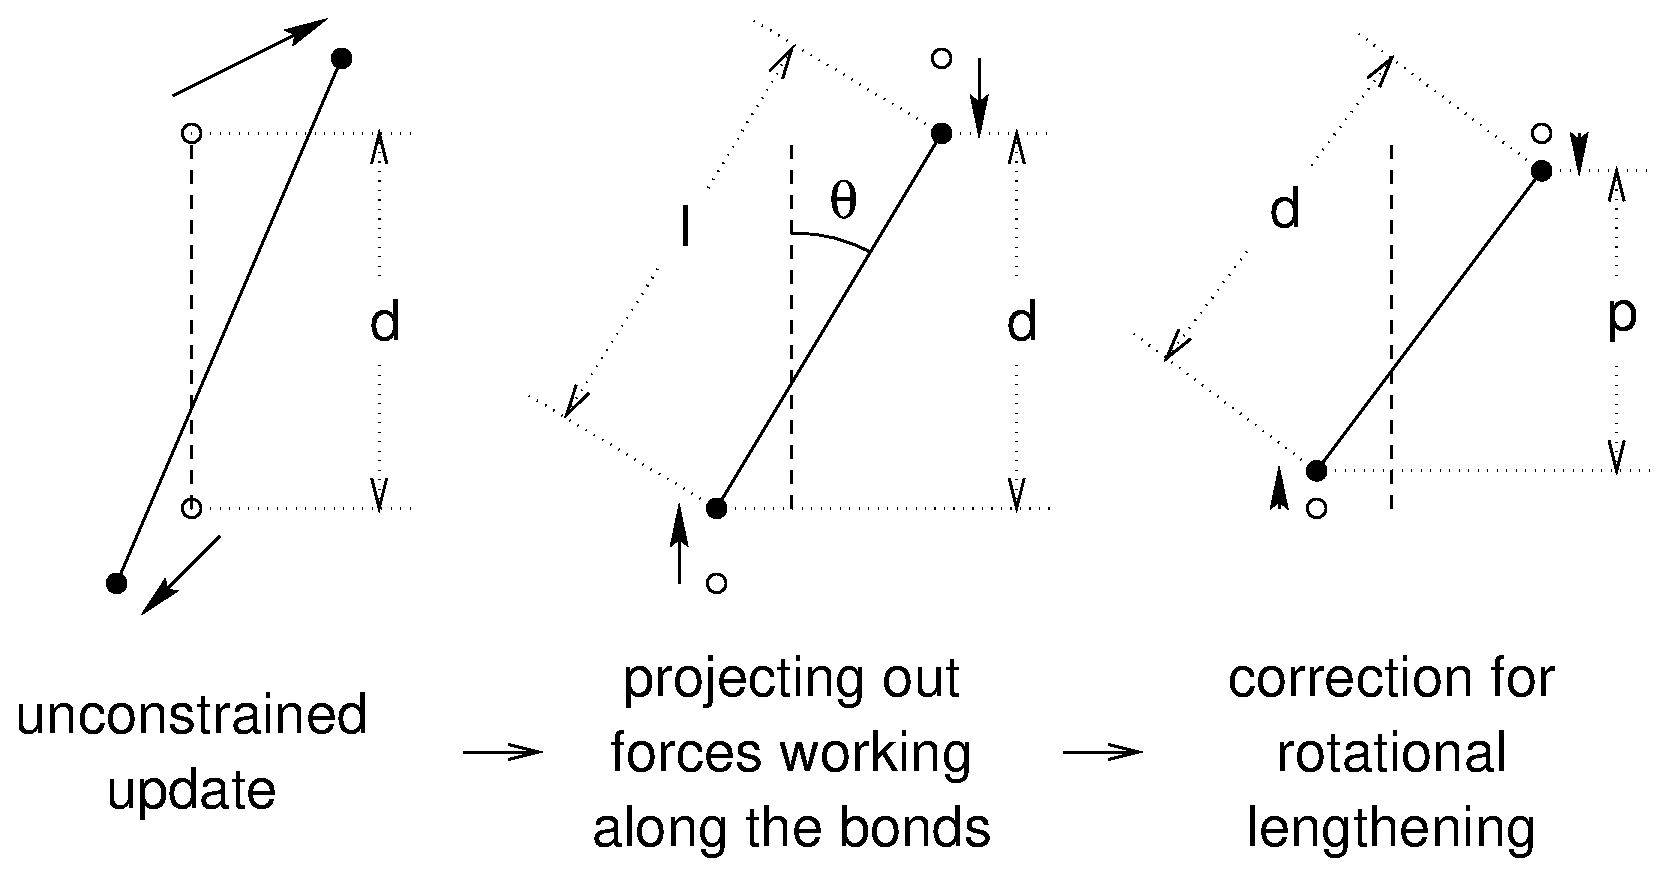
\includegraphics[height=50mm]{plots/lincs}}
\caption[The three position updates needed for one time step.]{The
three position updates needed for one time step. The dashed line is
the old bond of length $d$, the solid lines are the new bonds. $l=d
\cos \theta$ and $p=(2 d^2 - l^2)^{1 \over 2}$.}
\label{fig:lincs}
\end{figure}

A new notation is introduced for the gradient matrix of the constraint 
equations which appears on the right hand side of this equation:
\fs{c3}
B_{hi} = {\p g_h \over \p r_i}
\fe
Notice that $\Bm$ is a $K \times 3N$ matrix, it contains the directions
of the constraints.
The following equation shows how the new constrained coordinates 
$\ve{r}_{n+1}$ are related to the unconstrained coordinates
$\ve{r}_{n+1}^{unc}$ by
\fs{m0}
\begin{array}{c}
  \ve{r}_{n+1}=(\ve{I}-\Tm_n \ve{B}_n) \ve{r}_{n+1}^{unc} + \Tm_n \lenc=  
  \\[2mm]
  \ve{r}_{n+1}^{unc} - 
\iM \Bm_n (\Bm_n \iM \Bm_n^T)^{-1} (\Bm_n \ve{r}_{n+1}^{unc} - \lenc) 
\end{array}
\fe
where $\Tm = \iM \Bm^T (\Bm \iM \Bm^T)^{-1}$.
The derivation of this equation from \eqnsref{c1}{c2} can be found
in \cite{Hess97}.

This first step does not set the real bond lengths to the prescribed lengths,
but the projection of the new bonds onto the old directions of the bonds.
To correct for the rotation of bond $i$, the projection of the
bond, $p_i$, on the old direction is set to
\fs{m1a}
p_i=\sqrt{2 d_i^2 - l_i^2},
\fe
where $l_i$ is the bond length after the first projection.
The corrected positions are
\fs{m1b}
\ve{r}_{n+1}^*=(\ve{I}-\Tm_n \Bm_n)\ve{r}_{n+1} + \Tm_n \ve{p}.
\fe
This correction for rotational effects is actually an iterative process,
but during MD only one iteration is applied.
The relative constraint deviation after this procedure will be less than
0.0001 for every constraint.
In energy minimization, this might not be accurate enough, so the number
of iterations is equal to the order of the expansion (see below).

Half of the CPU time goes to inverting the constraint coupling 
matrix $\Bm_n \iM \Bm_n^T$, which has to be done every time step.
This $K \times K$ matrix
has $1/m_{i_1} + 1/m_{i_2}$ on the diagonal.
The off-diagonal elements are only non-zero when two bonds are connected,
then the element is 
$\cos \phi /m_c$,  where $m_c$ is 
the mass of the atom connecting the
two bonds and $\phi$ is the angle between the bonds.

The matrix $\Tm$ is inverted through a power expansion.
A $K \times K$ matrix $\ve{S}$ is 
introduced which is the inverse square root of 
the diagonal of $\Bm_n \iM \Bm_n^T$.
This matrix is used to convert the diagonal elements 
of the coupling matrix to one:
\fs{m2}
\begin{array}{c}
(\Bm_n \iM \Bm_n^T)^{-1}
= \Sm \Sm^{-1} (\Bm_n \iM \Bm_n^T)^{-1} \Sm^{-1} \Sm  \\[2mm]
= \Sm (\Sm \Bm_n \iM \Bm_n^T \Sm)^{-1} \Sm =
  \Sm (\ve{I} - \ve{A}_n)^{-1} \Sm
\end{array}
\fe
The matrix $\ve{A}_n$ is symmetric and sparse and has zeros on the diagonal.
Thus a simple trick can be used to calculate the inverse:
\fs{m3}
(\ve{I}-\ve{A}_n)^{-1}= 
        \ve{I} + \ve{A}_n + \ve{A}_n^2 + \ve{A}_n^3 + \ldots
\fe

This inversion method is only valid if the absolute values of all the
eigenvalues of $\ve{A}_n$ are smaller than one.
In molecules with only bond constraints, the connectivity is so low
that this will always be true, even if ring structures are present.
Problems can arise in angle-constrained molecules.
By constraining angles with additional distance constraints,
multiple small ring structures are introduced.
This gives a high connectivity, leading to large eigenvalues.
Therefore LINCS should NOT be used with coupled angle-constraints.

For molecules with all bonds constrained the eigenvalues of $A$
are around 0.4. This means that with each additional order
in the expansion \eqnref{m3} the deviations decrease by a factor 0.4.
But for relatively isolated triangles of constraints the largest
eigenvalue is around 0.7.
Such triangles can occur when removing hydrogen angle vibrations
with an additional angle constraint in alcohol groups
or when constraining water molecules with LINCS, for instance
with flexible constraints.
The constraints in such triangles converge twice as slow as
the other constraints. Therefore, starting with {\gromacs} 4,
additional terms are added to the expansion for such triangles
\fs{m3_ang}
(\ve{I}-\ve{A}_n)^{-1} \approx
        \ve{I} + \ve{A}_n + \ldots + \ve{A}_n^{N_i} +
        \left(\ve{A}^*_n + \ldots + {\ve{A}_n^*}^{N_i} \right) \ve{A}_n^{N_i}
\fe
where $N_i$ is the normal order of the expansion and
$\ve{A}^*$ only contains the elements of $\ve{A}$ that couple
constraints within rigid triangles, all other elements are zero.
In this manner, the accuracy of angle constraints comes close
to that of the other constraints, while the series of matrix vector
multiplications required for determining the expansion
only needs to be extended for a few constraint couplings.
This procedure is described in the P-LINCS paper\cite{Hess2008a}.

\subsubsection{The LINCS Parameters}
The accuracy of LINCS depends on the number of matrices used
in the expansion \eqnref{m3}. For MD calculations a fourth order
expansion is enough. For Brownian dynamics with
large time steps an eighth order expansion may be necessary.
The order is a parameter in the {\tt *.mdp} file.
The implementation of LINCS is done in such a way that the 
algorithm will never crash. Even when it is impossible to
to reset the constraints LINCS will generate a conformation
which fulfills the constraints as well as possible.
However, LINCS will generate a warning when in one step a bond 
rotates over more than a predefined angle.
This angle is set by the user in the {\tt *.mdp} file.

% } % Brace matches ifthenelse test for gmxlite


\section{Simulated Annealing}
\label{sec:SA}
The well known \swapindex{simulated}{annealing}
(SA) protocol is supported in {\gromacs}, and you can even couple multiple
groups of atoms separately with an arbitrary number of reference temperatures
that change during the simulation. The annealing is implemented by simply 
changing the current reference temperature for each group in the temperature
coupling, so the actual relaxation and coupling properties depends on the
type of thermostat you use and how hard you are coupling it. Since we are
changing the reference temperature it is important to remember that the system
will NOT instantaneously reach this value - you need to allow for the inherent
relaxation time in the coupling algorithm too. If you are changing the 
annealing reference temperature faster than the temperature relaxation you
will probably end up with a crash when the difference becomes too large.

The annealing protocol is specified as a series of corresponding times and 
reference temperatures for each group, and you can also choose whether you only
want a single sequence (after which the temperature will be coupled to the 
last reference value), or if the annealing should be periodic and restart at 
the first reference point once the sequence is completed. You can mix and
match both types of annealing and non-annealed groups in your simulation.

\newcommand{\vrond}{\stackrel{\circ}{\ve{r}}}
\newcommand{\rond}{\stackrel{\circ}{r}}
\newcommand{\ruis}{\ve{r}^G}

% \ifthenelse{\equal{\gmxlite}{1}}{}{
\section{Stochastic Dynamics\swapindexquiet{stochastic}{dynamics}}
\label{sec:SD}
Stochastic or velocity \swapindex{Langevin}{dynamics} adds a friction
and a noise term to Newton's equations of motion, as
\beq
\label{SDeq}
m_i {\de^2 \ve{r}_i \over \de t^2} =
- m_i \gamma_i {\de \ve{r}_i \over \de t} + \ve{F}_i(\ve{r}) + \vrond_i,
\eeq 
where $\gamma_i$ is the friction constant $[1/\mbox{ps}]$ and
$\vrond_i\!\!(t)$  is a noise process with 
$\langle \rond_i\!\!(t) \rond_j\!\!(t+s) \rangle = 
    2 m_i \gamma_i k_B T \delta(s) \delta_{ij}$.
When $1/\gamma_i$ is large compared to the time scales present in the system,
one could see stochastic dynamics as molecular dynamics with stochastic
temperature-coupling. The advantage compared to MD with Berendsen
temperature-coupling is that in case of SD the generated ensemble is known.
For simulating a system in vacuum there is the additional advantage that there is no
accumulation of errors for the overall translational and rotational
degrees of freedom.
When $1/\gamma_i$ is small compared to the time scales present in the system,
the dynamics will be completely different from MD, but the sampling is
still correct.

In {\gromacs} there is one simple and efficient implementation. Its
accuracy is equivalent to the normal MD leap-frog and
Velocity Verlet integrator. It is nearly identical to the common way of discretizing the Langevin equation, but the friction and velocity term are applied in an impulse fashion~\cite{Goga2012}.
It can be described as:
\bea
\label{eqn:sd_int1}
\ve{v}'  &~=~&   \ve{v}(t-\hDt) + \frac{1}{m}\ve{F}(t)\Dt \\
\Delta\ve{v}     &~=~&   -\alpha \, \ve{v}'(t+\hDt) + \sqrt{\frac{k_B T}{m}(1 - \alpha^2)} \, \ruis_i \\
\ve{r}(t+\Dt)   &~=~&   \ve{r}(t)+\left(\ve{v}' +\frac{1}{2}\Delta \ve{v}\right)\Dt \label{eqn:sd1_x_upd}\\
\ve{v}(t+\hDt)  &~=~&   \ve{v}' + \Delta \ve{v} \\
\alpha &~=~& 1 - e^{-\gamma \Dt}
\eea
where $\ruis_i$ is Gaussian distributed noise with $\mu = 0$, $\sigma = 1$.
The velocity is first updated a full time step without friction and noise to get $\ve{v}'$, identical to the normal update in leap-frog. The friction and noise are then applied as an impulse at step $t+\Dt$. The advantage of this scheme is that the velocity-dependent terms act at the full time step, which makes the correct integration of forces that depend on both coordinates and velocities, such as constraints and dissipative particle dynamics (DPD, not implented yet), straightforward. With constraints, the coordinate update \eqnref{sd1_x_upd} is split into a normal leap-frog update and a $\Delta \ve{v}$. After both of these updates the constraints are applied to coordinates and velocities.

When using SD as a thermostat, an appropriate value for $\gamma$ is e.g. 0.5 ps$^{-1}$,
since this results in a friction that is lower than the internal friction
of water, while it still provides efficient thermostatting.


\section{Brownian Dynamics\swapindexquiet{Brownian}{dynamics}}
\label{sec:BD}
In the limit of high friction, stochastic dynamics reduces to 
Brownian dynamics, also called position Langevin dynamics.
This applies to over-damped systems, 
{\ie} systems in which the inertia effects are negligible.
The equation is
\beq
{\de \ve{r}_i \over \de t} = \frac{1}{\gamma_i} \ve{F}_i(\ve{r}) + \vrond_i
\eeq 
where $\gamma_i$ is the friction coefficient $[\mbox{amu/ps}]$ and
$\vrond_i\!\!(t)$  is a noise process with 
$\langle \rond_i\!\!(t) \rond_j\!\!(t+s) \rangle = 
    2 \delta(s) \delta_{ij} k_B T / \gamma_i$.
In {\gromacs} the equations are integrated with a simple, explicit scheme
\beq
\ve{r}_i(t+\Delta t) = \ve{r}_i(t) +
        {\Delta t \over \gamma_i} \ve{F}_i(\ve{r}(t)) 
        + \sqrt{2 k_B T {\Delta t \over \gamma_i}}\, \ruis_i,
\eeq
where $\ruis_i$ is Gaussian distributed noise with $\mu = 0$, $\sigma = 1$.
The friction coefficients $\gamma_i$ can be chosen the same for all
particles or as $\gamma_i = m_i\,\gamma_i$, where the friction constants
$\gamma_i$ can be different for different groups of atoms. 
Because the system is assumed to be over-damped, large timesteps
can be used. LINCS should be used for the constraints since SHAKE
will not converge for large atomic displacements.
BD is an option of the {\tt mdrun} program.
% } % Brace matches ifthenelse test for gmxlite

\section{Energy Minimization}
\label{sec:EM}\index{energy minimization}%
Energy minimization in {\gromacs} can be done using steepest descent,
conjugate gradients, or l-bfgs (limited-memory
Broyden-Fletcher-Goldfarb-Shanno quasi-Newtonian minimizer...we
prefer the abbreviation). EM is just an option of the {\tt mdrun}
program.

\subsection{Steepest Descent\index{steepest descent}}
Although steepest descent is certainly not the most efficient
algorithm for searching, it is robust and easy to implement.

We define the vector $\ve{r}$ as the vector of all $3N$ coordinates.
Initially a maximum displacement $h_0$ ({\eg} 0.01 nm) must be given. 

First the forces $\ve{F}$ and potential energy are calculated.
New positions are calculated by
\beq
\ve{r}_{n+1} =  \ve{r}_n + \frac{\ve{F}_n}{\max (|\ve{F}_n|)} h_n,
\eeq
where $h_n$ is the maximum displacement and $\ve{F}_n$ is the force,
or the negative gradient of the  potential $V$. The notation $\max
(|\ve{F}_n|)$ means the largest of the absolute values of the force
components.  The forces and energy are again computed for the new positions \\
If ($V_{n+1} < V_n$) the new positions are accepted and $h_{n+1} = 1.2
h_n$. \\
If ($V_{n+1} \geq V_n$) the new positions are rejected and $h_n = 0.2 h_n$.

The algorithm stops when either a user-specified number of force 
evaluations has been performed ({\eg} 100), or when the maximum of the absolute
values of the force (gradient) components is smaller than a specified
value $\epsilon$.
Since force truncation produces some noise in the
energy evaluation, the stopping criterion should not be made too tight
to avoid endless iterations. A reasonable value for $\epsilon$ can be
estimated from the root mean square force $f$ a harmonic oscillator would exhibit at a
temperature $T$. This value is
\beq
  f = 2 \pi \nu \sqrt{ 2mkT},
\eeq
where $\nu$ is the oscillator frequency, $m$ the (reduced) mass, and
$k$ Boltzmann's constant. For a weak oscillator with a wave number of
100 cm$^{-1}$ and a mass of 10 atomic units, at a temperature of 1 K,
$f=7.7$ kJ~mol$^{-1}$~nm$^{-1}$. A value for $\epsilon$ between 1 and
10 is acceptable.   

% \ifthenelse{\equal{\gmxlite}{1}}{}{
\subsection{Conjugate Gradient\index{conjugate gradient}}
Conjugate gradient is slower than steepest descent in the early stages
of the minimization, but becomes more efficient closer to the energy
minimum.  The parameters and stop criterion are the same as for
steepest descent.  In {\gromacs} conjugate gradient can not be used
with constraints, including the SETTLE algorithm for
water~\cite{Miyamoto92}, as this has not been implemented. If water is
present it must be of a flexible model, which can be specified in the
{\tt *.mdp} file by {\tt define = -DFLEXIBLE}.

This is not really a restriction, since the accuracy of conjugate
gradient is only required for minimization prior to a normal-mode
analysis, which cannot be performed with constraints.  For most other
purposes steepest descent is efficient enough.
% } % Brace matches ifthenelse test for gmxlite

% \ifthenelse{\equal{\gmxlite}{1}}{}{
\subsection{\normindex{L-BFGS}}
The original BFGS algorithm works by successively creating better
approximations of the inverse Hessian matrix, and moving the system to
the currently estimated minimum. The memory requirements for this are
proportional to the square of the number of particles, so it is not
practical for large systems like biomolecules. Instead, we use the
L-BFGS algorithm of Nocedal~\cite{Byrd95a,Zhu97a}, which approximates
the inverse Hessian by a fixed number of corrections from previous
steps. This sliding-window technique is almost as efficient as the
original method, but the memory requirements are much lower -
proportional to the number of particles multiplied with the correction
steps. In practice we have found it to converge faster than conjugate
gradients, but due to the correction steps it is not yet parallelized.
It is also noteworthy that switched or shifted interactions usually
improve the convergence, since sharp cut-offs mean the potential
function at the current coordinates is slightly different from the
previous steps used to build the inverse Hessian approximation.
% } % Brace matches ifthenelse test for gmxlite

% \ifthenelse{\equal{\gmxlite}{1}}{}{
\section{Normal-Mode Analysis\index{normal-mode analysis}\index{NMA}}
Normal-mode analysis~\cite{Levitt83,Go83,BBrooks83b} 
can be performed using {\gromacs}, by diagonalization of the mass-weighted
\normindex{Hessian} $H$:
\bea
R^T M^{-1/2} H M^{-1/2} R   &=& \mbox{diag}(\lambda_1,\ldots,\lambda_{3N})
\\
\lambda_i &=& (2 \pi \omega_i)^2
\eea
where $M$ contains the atomic masses, $R$ is a matrix that contains
the eigenvectors as columns, $\lambda_i$ are the eigenvalues
and $\omega_i$ are the corresponding frequencies.

First the Hessian matrix, which is a $3N \times 3N$ matrix where $N$
is the number of atoms, needs to be calculated:
\bea
H_{ij}  &=&     \frac{\partial^2 V}{\partial x_i \partial x_j}
\eea
where $x_i$ and $x_j$ denote the atomic x, y or z coordinates.
In practice, this equation is not used, but the Hessian is
calculated numerically from the force as:
\bea
H_{ij} &=& -
  \frac{f_i({\bf x}+h{\bf e}_j) - f_i({\bf x}-h{\bf e}_j)}{2h}
\\
f_i     &=& - \frac{\partial V}{\partial x_i}
\eea
where ${\bf e}_j$ is the unit vector in direction $j$.
It should be noted that
for a usual normal-mode calculation, it is necessary to completely minimize 
the energy prior to computation of the Hessian.
The tolerance required depends on the type of system,
but a rough indication is 0.001 kJ mol$^{-1}$.
Minimization should be done with conjugate gradients or L-BFGS in double precision.

A number of {\gromacs} programs are involved in these
calculations. First, the energy should be minimized using {\tt mdrun}.
Then, {\tt mdrun} computes the Hessian.  {\bf Note} that for generating
the run input file, one should use the minimized conformation from
the full precision trajectory file, as the structure file is not
accurate enough.
{\tt \normindex{g_nmeig}} does the diagonalization and
the sorting of the normal modes according to their frequencies.
Both {\tt mdrun} and {\tt g_nmeig} should be run in double precision.
The normal modes can be analyzed with the program {\tt g_anaeig}.
Ensembles of structures at any temperature and for any subset of
normal modes can be generated with {\tt \normindex{g_nmens}}.
An overview of normal-mode analysis and the related principal component
analysis (see \secref{covanal}) can be found in~\cite{Hayward95b}.
% } % Brace matches ifthenelse test for gmxlite

% \ifthenelse{\equal{\gmxlite}{1}}{}{

\section{Free energy calculations\index{free energy calculations}}
\label{sec:fecalc}
\subsection{Slow-growth methods\index{slow-growth methods}}
Free energy calculations can be performed
in {\gromacs} using  a number of methods, including ``slow-growth.'' An example problem 
might be calculating the difference in free energy of binding of an inhibitor {\bf I}
to an enzyme {\bf E} and to a mutated enzyme {\bf E$^{\prime}$}. It 
is not feasible with computer simulations to perform a docking
calculation for such a large complex, or even releasing the inhibitor from
the enzyme in a reasonable amount of computer time with reasonable accuracy.
However, if we consider the free energy cycle in~\figref{free}A
we can write:
\beq
\Delta G_1 - \Delta G_2 =       \Delta G_3 - \Delta G_4
\label{eqn:ddg}
\eeq
If we are interested in the left-hand term we can equally well compute
the right-hand term.
\begin{figure}
\centerline{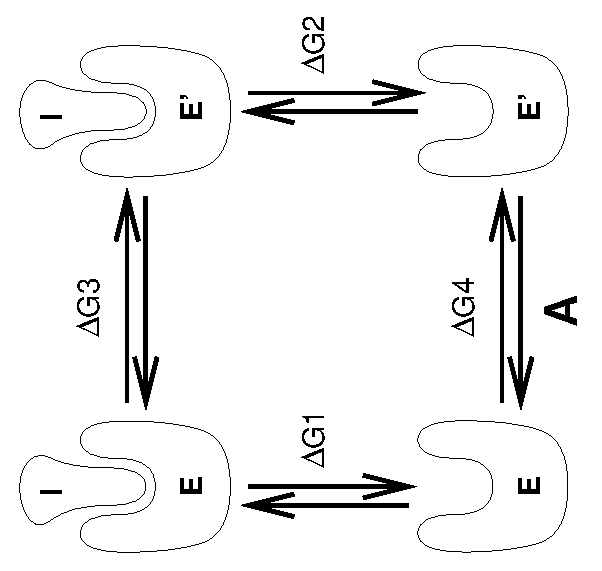
\includegraphics[width=6cm,angle=270]{plots/free1}\hspace{2cm}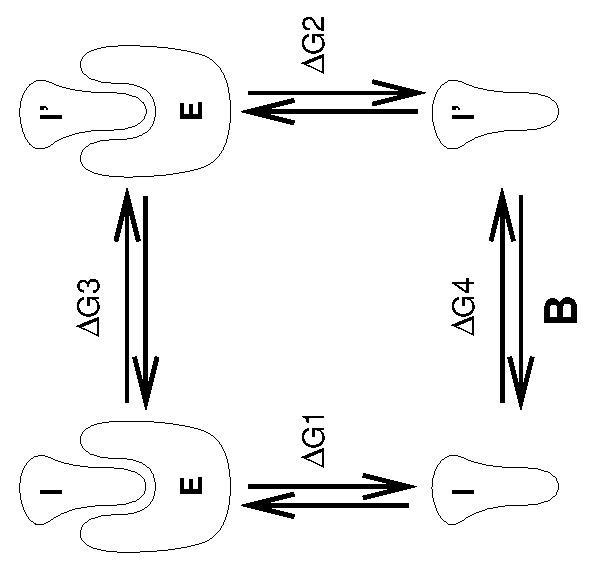
\includegraphics[width=6cm,angle=270]{plots/free2}}
\caption[Free energy cycles.]{Free energy cycles. {\bf A:} to
calculate $\Delta G_{12}$, the free energy difference between the
binding of inhibitor {\bf I} to enzymes {\bf E} respectively {\bf
E$^{\prime}$}. {\bf B:} to calculate $\Delta G_{12}$, the free energy
difference for binding of inhibitors {\bf I} respectively {\bf I$^{\prime}$} to
enzyme {\bf E}.}
\label{fig:free}
\end{figure}

If we want to compute the difference in free energy of binding of two
inhibitors {\bf I} and {\bf I$^{\prime}$} to an enzyme {\bf E} (\figref{free}B)
we can again use \eqnref{ddg} to compute the desired property.

\newcommand{\sA}{^{\mathrm{A}}}
\newcommand{\sB}{^{\mathrm{B}}}
Free energy differences between two molecular species can
be calculated in {\gromacs} using the ``slow-growth'' method.
Such free energy differences between different molecular species are
physically meaningless, but they can be used to obtain meaningful
quantities employing a thermodynamic cycle.
The method requires a simulation during which the Hamiltonian of the
system changes slowly from that describing one system (A) to that
describing the other system (B). The change must be so slow that the
system remains in equilibrium during the process; if that requirement
is fulfilled, the change is reversible and a slow-growth simulation from B to A
will yield the same results (but with a different sign) as a slow-growth
simulation from A to B. This is a useful check, but the user should be
aware of the danger that equality of forward and backward growth results does
not guarantee correctness of the results.

The required modification of the Hamiltonian $H$ is realized by making
$H$ a function of a \textit{coupling parameter} $\lambda:
H=H(p,q;\lambda)$ in such a way that $\lambda=0$ describes system A
and $\lambda=1$ describes system B: 
\beq
  H(p,q;0)=H\sA (p,q);~~~~ H(p,q;1)=H\sB (p,q).
\eeq
In {\gromacs}, the functional form of the $\lambda$-dependence is
different for the various force-field contributions and is described
in section \secref{feia}.

The Helmholtz free energy $A$ is related to the
partition function $Q$ of an $N,V,T$ ensemble, which is assumed to be
the equilibrium ensemble generated by a MD simulation at constant
volume and temperature. The generally more useful Gibbs free energy
$G$ is related to the partition function $\Delta$ of an $N,p,T$
ensemble, which is assumed to be the equilibrium ensemble generated by
a MD simulation at constant pressure and temperature:
\bea
 A(\lambda) &=&  -k_BT \ln Q \\
 Q &=& c \int\!\!\int \exp[-\beta H(p,q;\lambda)]\,dp\,dq \\
 G(\lambda) &=&  -k_BT \ln \Delta \\
 \Delta &=& c \int\!\!\int\!\!\int \exp[-\beta H(p,q;\lambda) -\beta
pV]\,dp\,dq\,dV \\
G &=& A + pV, 
\eea
where $\beta = 1/(k_BT)$ and $c = (N! h^{3N})^{-1}$.
These integrals over phase space cannot be evaluated from a
simulation, but it is possible to evaluate the derivative with 
respect to $\lambda$ as an ensemble average:
\beq
 \frac{dA}{d\lambda} =  \frac{\int\!\!\int (\partial H/ \partial
\lambda) \exp[-\beta H(p,q;\lambda)]\,dp\,dq}{\int\!\!\int \exp[-\beta
H(p,q;\lambda)]\,dp\,dq} = 
\left\langle \frac{\partial H}{\partial \lambda} \right\rangle_{NVT;\lambda},
\eeq
with a similar relation for $dG/d\lambda$ in the $N,p,T$
ensemble.  The difference in free energy between A and B can be found
by integrating the derivative over $\lambda$:
\bea
  A\sB(V,T)-A\sA(V,T) &=& \int_0^1 \left\langle \frac{\partial
H}{\partial \lambda} \right\rangle_{NVT;\lambda} \,d\lambda 
\label{eq:delA} \\
 G\sB(p,T)-G\sA(p,T) &=& \int_0^1 \left\langle \frac{\partial
H}{\partial \lambda} \right\rangle_{NpT;\lambda} \,d\lambda.
\label{eq:delG}
\eea
If one wishes to evaluate $G\sB(p,T)-G\sA(p,T)$,
the natural choice is a constant-pressure simulation. However, this
quantity can also be obtained from a slow-growth simulation at
constant volume, starting with system A at pressure $p$ and volume $V$
and ending with system B at pressure $p_B$, by applying the following
small (but, in principle, exact) correction: 
\beq
  G\sB(p)-G\sA(p) =
A\sB(V)-A\sA(V) - \int_p^{p\sB}[V\sB(p')-V]\,dp'
\eeq
Here we omitted the constant $T$ from the notation. This correction is
roughly equal to $-\frac{1}{2} (p\sB-p)\Delta V=(\Delta V)^2/(2
\kappa V)$, where $\Delta V$ is the volume change at $p$ and $\kappa$
is the isothermal compressibility. This is usually
small; for example, the growth of a water molecule from nothing
in a bath of 1000 water molecules at constant volume would produce an
additional pressure of as much as 22 bar, but a correction to the 
Helmholtz free energy of just -1 kJ mol$^{-1}$. %-20 J/mol.

In Cartesian coordinates, the kinetic energy term in the Hamiltonian
depends only on the momenta, and can be separately integrated and, in
fact, removed from the equations. When masses do not change, there is
no contribution from the kinetic energy at all; otherwise the
integrated contribution to the free energy is $-\frac{3}{2} k_BT \ln
(m\sB/m\sA)$. {\bf Note} that this is only true in the absence of constraints.

\subsection{Thermodynamic integration\index{thermodynamic integration}\index{BAR}\index{Bennett's acceptance ratio}}  
{\gromacs} offers the possibility to integrate eq.~\ref{eq:delA} or
eq. \ref{eq:delG} in one simulation over the full range from A to
B. However, if the change is large and insufficient sampling can be
expected, the user may prefer to determine the value of $\langle
dG/d\lambda \rangle$ accurately at a number of well-chosen
intermediate values of $\lambda$. This can easily be done by setting
the stepsize {\tt delta_lambda} to zero. Each simulation can be
equilibrated first, and a proper error estimate can be made for each
value of $dG/d\lambda$ from the fluctuation of $\partial H/\partial
\lambda$. The total free energy change is then determined afterward
by an appropriate numerical integration procedure.

{\gromacs} now also supports the use of Bennett's Acceptance Ratio~\cite{Bennett1976}
for calculating values of $\Delta$G for transformations from state A to state B using
the program {\tt \normindex{g_bar}}. The same data can also be used to calculate free
energies using MBAR~\cite{Shirts2008}, though the analysis currently requires external tools from
the external {\tt pymbar} package, at https://SimTK.org/home/pymbar.

The $\lambda$-dependence for the force-field contributions is
described in detail in section \secref{feia}.
% } % Brace matches ifthenelse test for gmxlite

% \ifthenelse{\equal{\gmxlite}{1}}{}{
\section{Replica exchange\index{replica exchange}}
Replica exchange molecular dynamics (\normindex{REMD})
is a method that can be used to speed up
the sampling of any type of simulation, especially if
conformations are separated by relatively high energy barriers.
It involves simulating multiple replicas of the same system
at different temperatures and randomly exchanging the complete state
of two replicas at regular intervals with the probability:
\beq
P(1 \leftrightarrow 2)=\min\left(1,\exp\left[
\left(\frac{1}{k_B T_1} - \frac{1}{k_B T_2}\right)(U_1 - U_2)
 \right] \right)
\eeq
where $T_1$ and $T_2$ are the reference temperatures and $U_1$ and $U_2$
are the instantaneous potential energies of replicas 1 and 2 respectively.
After exchange the velocities are scaled by $(T_1/T_2)^{\pm0.5}$
and a neighbor search is performed the next step.
This combines the fast sampling and frequent barrier-crossing
of the highest temperature with correct Boltzmann sampling at
all the different temperatures~\cite{Hukushima96a,Sugita99}.
We only attempt exchanges for neighboring temperatures as the probability
decreases very rapidly with the temperature difference.
One should not attempt exchanges for all possible pairs in one step.
If, for instance, replicas 1 and 2 would exchange, the chance of
exchange for replicas 2 and 3 not only depends on the energies of
replicas 2 and 3, but also on the energy of replica 1.
In {\gromacs} this is solved by attempting exchange for all ``odd''
pairs on ``odd'' attempts and for all ``even'' pairs on ``even'' attempts.
If we have four replicas: 0, 1, 2 and 3, ordered in temperature
and we attempt exchange every 1000 steps, pairs 0-1 and 2-3
will be tried at steps 1000, 3000 etc. and pair 1-2 at steps 2000, 4000 etc.

How should one choose the temperatures?
The energy difference can be written as:
\beq
U_1 - U_2 =  N_{df} \frac{c}{2} k_B (T_1 - T_2)
\eeq
where $N_{df}$ is the total number of degrees of freedom of one replica
and $c$ is 1 for harmonic potentials and around 2 for protein/water systems.
If $T_2 = (1+\epsilon) T_1$ the probability becomes:
\beq
P(1 \leftrightarrow 2)
  = \exp\left( -\frac{\epsilon^2 c\,N_{df}}{2 (1+\epsilon)} \right)
\approx \exp\left(-\epsilon^2 \frac{c}{2} N_{df} \right)
\eeq
Thus for a probability of $e^{-2}\approx 0.135$
one obtains $\epsilon \approx 2/\sqrt{c\,N_{df}}$.
With all bonds constrained one has $N_{df} \approx 2\, N_{atoms}$
and thus for $c$ = 2 one should choose $\epsilon$ as $1/\sqrt{N_{atoms}}$.
However there is one problem when using pressure coupling. The density at
higher temperatures will decrease, leading to higher energy~\cite{Seibert2005a},
which should be taken into account. The {\gromacs} website features a
so-called ``REMD calculator,'' that lets you type in the temperature range and
the number of atoms, and based on that proposes a set of temperatures.

An extension to the REMD for the isobaric-isothermal ensemble was
proposed by Okabe {\em et al.}~\cite{Okabe2001a}. In this work the
exchange probability is modified to:
\beq
P(1 \leftrightarrow 2)=\min\left(1,\exp\left[
\left(\frac{1}{k_B T_1} - \frac{1}{k_B T_2}\right)(U_1 - U_2) +
\left(\frac{P_1}{k_B T_1} - \frac{P_2}{k_B T_2}\right)\left(V_1-V_2\right)
 \right] \right)
\eeq
where $P_1$ and $P_2$ are the respective reference pressures and $V_1$ and
$V_2$ are the respective instantaneous volumes in the simulations.
In most cases the differences in volume are so small that the second
term is negligible. It only plays a role when the difference between
$P_1$ and $P_2$ is large or in phase transitions.

Hamiltonian replica exchange is also supported in {\gromacs}.  In
Hamiltonian replica exchange, each replica has a different
Hamiltonian, defined by the free energy pathway specified for the simulation.  The
exchange probability to maintain the correct ensemble probabilities is:
\beq P(1 \leftrightarrow 2)=\min\left(1,\exp\left[
    \left(\frac{1}{k_B T} - \frac{1}{k_B T}\right)((U_1(x_2) - U_1(x_1)) + (U_2(x_1) - U_2(x_2)))
\right]
\right)
\eeq
The separate Hamiltonians are defined by the free energy functionality
of {\gromacs}, with swaps made between the different values of
$\lambda$ defined in the mdp file.

Hamiltonian and temperature replica exchange can also be performed
simultaneously, using the acceptance criteria:
\beq
P(1 \leftrightarrow 2)=\min\left(1,\exp\left[
\left(\frac{1}{k_B T} - \right)(\frac{U_1(x_2) - U_1(x_1)}{k_B T_1} + \frac{U_2(x_1) - U_2(x_2)}{k_B T_2})
 \right] \right)
\eeq

Gibbs sampling replica exchange has also been implemented in
{\gromacs}~\cite{Chodera2011}.  In Gibbs sampling replica exchange, all
possible pairs are tested for exchange, allowing swaps between
replicas that are not neighbors.

Gibbs sampling replica exchange requires no additional potential
energy calculations.  However there is an additional communication
cost in Gibbs sampling replica exchange, as for some permutations,
more than one round of swaps must take place.  In some cases, this
extra communication cost might affect the efficiency.

All replica exchange variants are options of the {\tt mdrun}
program. It will only work when MPI is installed, due to the inherent
parallelism in the algorithm. For efficiency each replica can run on a
separate rank.  See the manual page of {\tt mdrun} on how to use these
multinode features.

% \ifthenelse{\equal{\gmxlite}{1}}{}{

\section{Essential Dynamics sampling\index{essential dynamics}\index{principal component analysis}\seeindexquiet{PCA}{covariance analysis}}
The results from Essential Dynamics (see \secref{covanal})
of a protein can be used to guide MD simulations. The idea is that
from an initial MD simulation (or from other sources) a definition of
the collective fluctuations with largest amplitude is obtained. The
position along one or more of these collective modes can be
constrained in a (second) MD simulation in a number of ways for
several purposes. For example, the position along a certain mode may
be kept fixed to monitor the average force (free-energy gradient) on
that coordinate in that position. Another application is to enhance
sampling efficiency with respect to usual MD
\cite{Degroot96a,Degroot96b}. In this case, the system is encouraged
to sample its available configuration space more systematically than
in a diffusion-like path that proteins usually take.

Another possibility to enhance sampling is \normindex{flooding}.
Here a flooding potential is added to certain
(collective) degrees of freedom to expel the system out
of a region of phase space \cite{Lange2006a}.

The procedure for essential dynamics sampling or flooding is as follows.
First, the eigenvectors and eigenvalues need to be determined
using covariance analysis ({\tt g_covar})
or normal-mode analysis ({\tt g_nmeig}).
Then, this information is fed into {\tt make_edi},
which has many options for selecting vectors and setting parameters,
see {\tt gmx make_edi -h}.
The generated {\tt edi} input file is then passed to {\tt mdrun}.

% } % Brace matches ifthenelse test for gmxlite

% \ifthenelse{\equal{\gmxlite}{1}}{}{
\section{\normindex{Expanded Ensemble}}

In an expanded ensemble simulation~\cite{Lyubartsev1992}, both the coordinates and the
thermodynamic ensemble are treated as configuration variables that can
be sampled over.  The probability of any given state can be written as:
\beq
P(\vec{x},k) \propto \exp\left(-\beta_k U_k + g_k\right),
\eeq
where $\beta_k = \frac{1}{k_B T_k}$ is the $\beta$ corresponding to the $k$th
thermodynamic state, and $g_k$ is a user-specified weight factor corresponding
to the $k$th state.  This space is therefore a {\em mixed}, {\em generalized}, or {\em
  expanded} ensemble which samples from multiple thermodynamic
ensembles simultaneously. $g_k$ is chosen to give a specific weighting
of each subensemble in the expanded ensemble, and can either be fixed,
or determined by an iterative procedure. The set of $g_k$ is
frequently chosen to give each thermodynamic ensemble equal
probability, in which case $g_k$ is equal to the free energy in
non-dimensional units, but they can be set to arbitrary values as
desired.  Several different algorithms can be used to equilibrate
these weights, described in the mdp option listings.
% } % Brace matches ifthenelse test for gmxlite

In {\gromacs}, this space is sampled by alternating sampling in the $k$
and $\vec{x}$ directions.  Sampling in the $\vec{x}$ direction is done
by standard molecular dynamics sampling; sampling between the
different thermodynamics states is done by Monte Carlo, with several
different Monte Carlo moves supported. The $k$ states can be defined
by different temperatures, or choices of the free energy $\lambda$
variable, or both.  Expanded ensemble simulations thus represent a
serialization of the replica exchange formalism, allowing a single
simulation to explore many thermodynamic states.



\section{Parallelization\index{parallelization}}
The CPU time required for a simulation can be reduced by running the simulation
in parallel over more than one core.
Ideally, one would want to have linear scaling: running on $N$ cores
makes the simulation $N$ times faster. In practice this can only be
achieved for a small number of cores. The scaling will depend
a lot on the algorithms used. Also, different algorithms can have different
restrictions on the interaction ranges between atoms.

\section{Domain decomposition\index{domain decomposition}}
Since most interactions in molecular simulations are local,
domain decomposition is a natural way to decompose the system.
In domain decomposition, a spatial domain is assigned to each rank,
which will then integrate the equations of motion for the particles
that currently reside in its local domain. With domain decomposition,
there are two choices that have to be made: the division of the unit cell
into domains and the assignment of the forces to domains.
Most molecular simulation packages use the half-shell method for assigning
the forces. But there are two methods that always require less communication:
the eighth shell~\cite{Liem1991} and the midpoint~\cite{Shaw2006} method.
{\gromacs} currently uses the eighth shell method, but for certain systems
or hardware architectures it might be advantageous to use the midpoint
method. Therefore, we might implement the midpoint method in the future.
Most of the details of the domain decomposition can be found
in the {\gromacs} 4 paper~\cite{Hess2008b}.

\subsection{Coordinate and force communication}
In the most general case of a triclinic unit cell,
the space in divided with a 1-, 2-, or 3-D grid in parallelepipeds
that we call domain decomposition cells.
Each cell is assigned to a particle-particle rank.
The system is partitioned over the ranks at the beginning
of each MD step in which neighbor searching is performed.
Since the neighbor searching is based on charge groups, charge groups
are also the units for the domain decomposition.
Charge groups are assigned to the cell where their center of geometry resides.
Before the forces can be calculated, the coordinates from some
neighboring cells need to be communicated,
and after the forces are calculated, the forces need to be communicated
in the other direction.
The communication and force assignment is based on zones that 
can cover one or multiple cells.
An example of a zone setup is shown in \figref{ddcells}.

\begin{figure}
\centerline{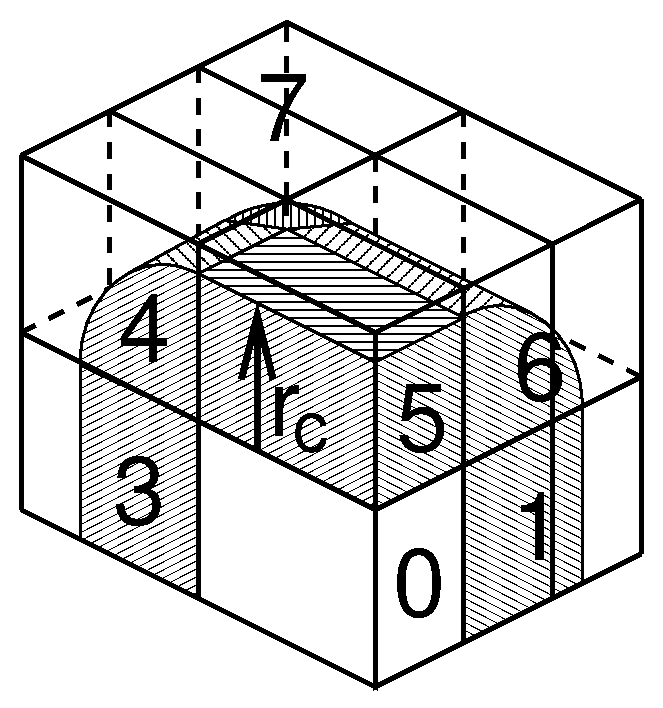
\includegraphics[width=6cm]{plots/dd-cells}}
\caption{
A non-staggered domain decomposition grid of 3$\times$2$\times$2 cells.
Coordinates in zones 1 to 7 are communicated to the corner cell
that has its home particles in zone 0.
$r_c$ is the cut-off radius. 
\label{fig:ddcells}
}
\end{figure}

The coordinates are communicated by moving data along the ``negative''
direction in $x$, $y$ or $z$ to the next neighbor. This can be done in one
or multiple pulses. In \figref{ddcells} two pulses in $x$ are required,
then one in $y$ and then one in $z$. The forces are communicated by
reversing this procedure. See the {\gromacs} 4 paper~\cite{Hess2008b}
for details on determining which non-bonded and bonded forces
should be calculated on which rank.

\subsection{Dynamic load balancing\swapindexquiet{dynamic}{load balancing}}
When different ranks have a different computational load
(load imbalance), all ranks will have to wait for the one
that takes the most time. One would like to avoid such a situation.
Load imbalance can occur due to four reasons:
\begin{itemize}
\item inhomogeneous particle distribution
\item inhomogeneous interaction cost distribution (charged/uncharged,
  water/non-water due to {\gromacs} water innerloops)
\item statistical fluctuation (only with small particle numbers)
\item differences in communication time, due to network topology and/or other jobs on the machine interfering with our communication
\end{itemize}
So we need a dynamic load balancing algorithm
where the volume of each domain decomposition cell
can be adjusted {\em independently}.
To achieve this, the 2- or 3-D domain decomposition grids need to be
staggered. \figref{ddtric} shows the most general case in 2-D.
Due to the staggering, one might require two distance checks
for deciding if a charge group needs to be communicated:
a non-bonded distance and a bonded distance check.

\begin{figure}
\centerline{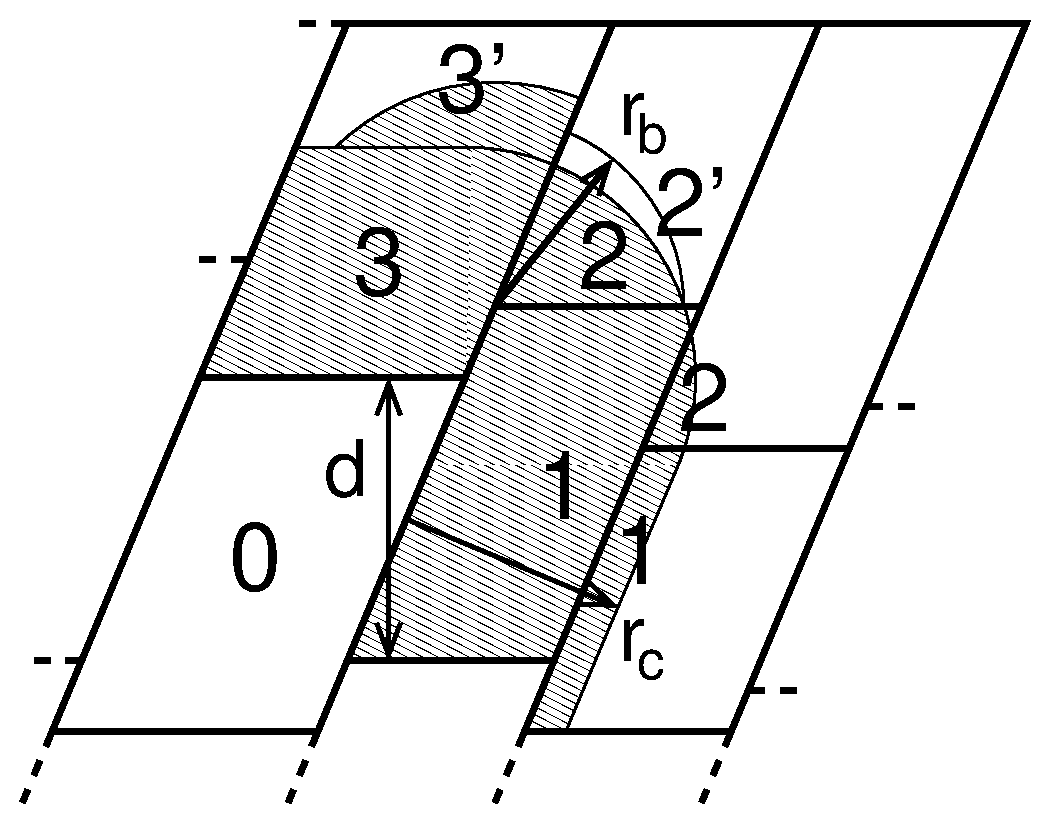
\includegraphics[width=7cm]{plots/dd-tric}}
\caption{
The zones to communicate to the rank of zone 0,
see the text for details. $r_c$ and $r_b$ are the non-bonded
and bonded cut-off radii respectively, $d$ is an example
of a distance between following, staggered boundaries of cells.
\label{fig:ddtric}
}
\end{figure}

By default, {\tt mdrun} automatically turns on the dynamic load
balancing during a simulation when the total performance loss
due to the force calculation imbalance is 2\% or more.
{\bf Note} that the reported force load imbalance numbers might be higher,
since the force calculation is only part of work that needs to be done
during an integration step.
The load imbalance is reported in the log file at log output steps
and when the {\tt -v} option is used also on screen.
The average load imbalance and the total performance loss
due to load imbalance are reported at the end of the log file.

There is one important parameter for the dynamic load balancing,
which is the minimum allowed scaling. By default, each dimension
of the domain decomposition cell can scale down by at least
a factor of 0.8. For 3-D domain decomposition this allows cells
to change their volume by about a factor of 0.5, which should allow
for compensation of a load imbalance of 100\%.
The minimum allowed scaling can be changed with the {\tt -dds}
option of {\tt mdrun}.

The load imbalance is measured by timing a single region of the MD step
on each MPI rank. This region can not include MPI communication, as
timing of MPI calls does not allow separating wait due to imbalance
from actual communication.
The domain volumes are then scaled, with under-relaxation, inversely
proportional with the measured time. This procedure will decrease the
load imbalance when the change in load in the measured region correlates
with the change in domain volume and the load outside
the measured region does not depend strongly on the domain volume.
In CPU-only simulations, the load is measured between the coordinate
and the force communication. In hybrid CPU-GPU simulations we overlap
communication on the CPU with calculation on the GPU. Therefore we
measure from the last communication before the force calculation to
when the CPU or GPU is finished, whichever is last.
When not using PME ranks, we subtract the time in PME from the CPU time,
as this includes MPI calls and the PME load is independent of domain size.
This generally works well, unless the non-bonded load is low and there is
imbalance in the bonded interactions. Then two issues can arise.
Dynamic load balancing can increase the imbalance in update and constraints
and with PME the coordinate and force redistribution time can go up
significantly. Although dynamic load balancing
can significantly improve performance in cases where there is imbalance in
the bonded interactions on the CPU, there are many situations in which
some domains continue decreasing in size and the load imbalance increases
and/or PME coordinate and force redistribution cost increases significantly.
As of version 2016.1, {\tt mdrun} disables the dynamic load balancing when
measurement indicates that it deteriorates performance. This means that in most
cases the user will get good performance with the default, automated
dynamic load balancing setting.

\subsection{Constraints in parallel\index{constraints}}
\label{subsec:plincs}
Since with domain decomposition parts of molecules can reside
on different ranks, bond constraints can cross cell boundaries.
Therefore a parallel constraint algorithm is required.
{\gromacs} uses the \normindex{P-LINCS} algorithm~\cite{Hess2008a},
which is the parallel version of the \normindex{LINCS} algorithm~\cite{Hess97}
% \ifthenelse{\equal{\gmxlite}{1}}
{.}
{(see \ssecref{lincs}).}
The P-LINCS procedure is illustrated in \figref{plincs}.
When molecules cross the cell boundaries, atoms in such molecules
up to ({\tt lincs_order + 1}) bonds away are communicated over the cell boundaries.
Then, the normal LINCS algorithm can be applied to the local bonds
plus the communicated ones. After this procedure, the local bonds
are correctly constrained, even though the extra communicated ones are not.
One coordinate communication step is required for the initial LINCS step
and one for each iteration. Forces do not need to be communicated.

\begin{figure}
\centerline{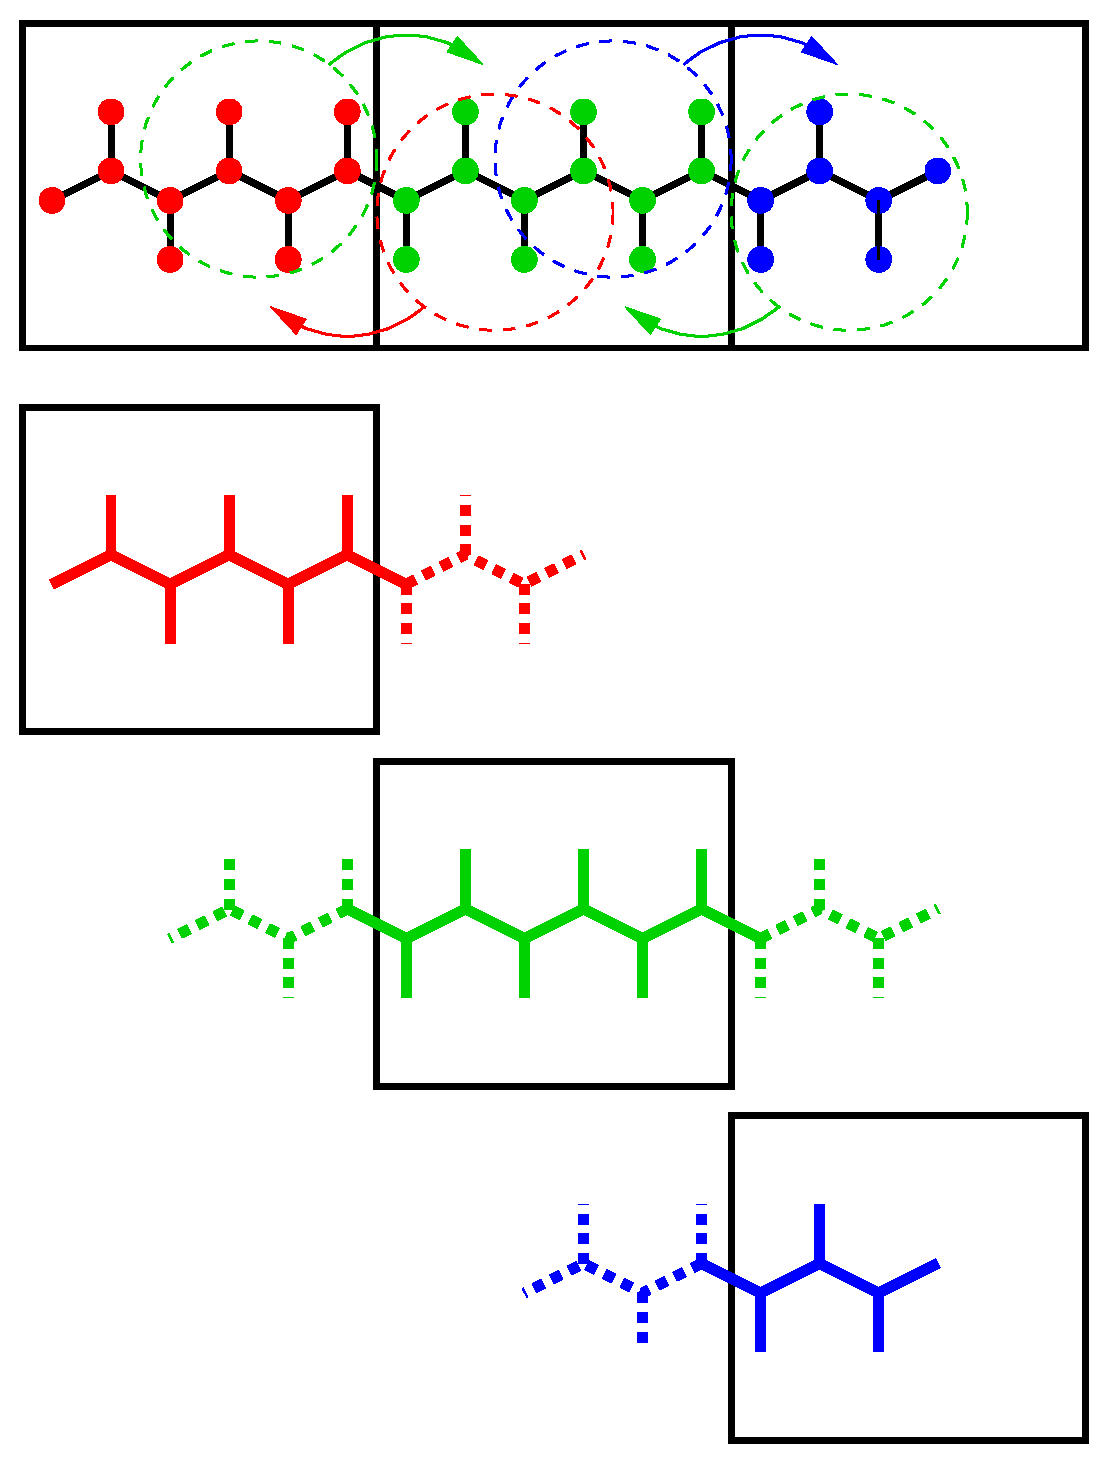
\includegraphics[width=6cm]{plots/par-lincs2}}
\caption{
Example of the parallel setup of P-LINCS with one molecule
split over three domain decomposition cells, using a matrix
expansion order of 3.
The top part shows which atom coordinates need to be communicated
to which cells. The bottom parts show the local constraints (solid)
and the non-local constraints (dashed) for each of the three cells.
\label{fig:plincs}
}
\end{figure}

\subsection{Interaction ranges}
Domain decomposition takes advantage of the locality of interactions.
This means that there will be limitations on the range of interactions.
By default, {\tt mdrun} tries to find the optimal balance between
interaction range and efficiency. But it can happen that a simulation
stops with an error message about missing interactions,
or that a simulation might run slightly faster with shorter
interaction ranges. A list of interaction ranges
and their default values is given in \tabref{dd_ranges}.

\begin{table}
\centerline{
\begin{tabular}{|c|c|ll|}
\dline
interaction & range & option & default \\
\dline
non-bonded        & $r_c$ = max($r_{\mathrm{list}}$,$r_{\mathrm{VdW}}$,$r_{\mathrm{Coul}}$) & {\tt mdp} file & \\
two-body bonded   & max($r_{\mathrm{mb}}$,$r_c$) & {\tt mdrun -rdd} & starting conf. + 10\% \\
multi-body bonded & $r_{\mathrm{mb}}$ & {\tt mdrun -rdd} & starting conf. + 10\% \\
constraints       & $r_{\mathrm{con}}$ & {\tt mdrun -rcon} & est. from bond lengths \\
virtual sites     & $r_{\mathrm{con}}$ & {\tt mdrun -rcon} & 0 \\
\dline
\end{tabular}
}
\caption{The interaction ranges with domain decomposition.}
\label{tab:dd_ranges}
\end{table}

In most cases the defaults of {\tt mdrun} should not cause the simulation
to stop with an error message of missing interactions.
The range for the bonded interactions is determined from the distance
between bonded charge-groups in the starting configuration, with 10\% added
for headroom. For the constraints, the value of $r_{\mathrm{con}}$ is determined by
taking the maximum distance that ({\tt lincs_order + 1}) bonds can cover
when they all connect at angles of 120 degrees.
The actual constraint communication is not limited by $r_{\mathrm{con}}$,
but by the minimum cell size $L_C$, which has the following lower limit:
\beq
L_C \geq \max(r_{\mathrm{mb}},r_{\mathrm{con}})
\eeq
Without dynamic load balancing the system is actually allowed to scale
beyond this limit when pressure scaling is used.
{\bf Note} that for triclinic boxes, $L_C$ is not simply the box diagonal
component divided by the number of cells in that direction,
rather it is the shortest distance between the triclinic cells borders.
For rhombic dodecahedra this is a factor of $\sqrt{3/2}$ shorter
along $x$ and $y$.

When $r_{\mathrm{mb}} > r_c$, {\tt mdrun} employs a smart algorithm to reduce
the communication. Simply communicating all charge groups within
$r_{\mathrm{mb}}$ would increase the amount of communication enormously.
Therefore only charge-groups that are connected by bonded interactions
to charge groups which are not locally present are communicated.
This leads to little extra communication, but also to a slightly
increased cost for the domain decomposition setup.
In some cases, {\eg} coarse-grained simulations with a very short cut-off,
one might want to set $r_{\mathrm{mb}}$ by hand to reduce this cost.

\subsection{Multiple-Program, Multiple-Data PME parallelization\index{PME}}
\label{subsec:mpmd_pme}
Electrostatics interactions are long-range, therefore special
algorithms are used to avoid summation over many atom pairs.
In {\gromacs} this is usually
% \ifthenelse{\equal{\gmxlite}{1}}
{.}
{PME (\secref{pme}).}
Since with PME all particles interact with each other, global communication
is required. This will usually be the limiting factor for 
scaling with domain decomposition.
To reduce the effect of this problem, we have come up with
a Multiple-Program, Multiple-Data approach~\cite{Hess2008b}.
Here, some ranks are selected to do only the PME mesh calculation,
while the other ranks, called particle-particle (PP) ranks,
do all the rest of the work.
For rectangular boxes the optimal PP to PME rank ratio is usually 3:1,
for rhombic dodecahedra usually 2:1.
When the number of PME ranks is reduced by a factor of 4, the number
of communication calls is reduced by about a factor of 16.
Or put differently, we can now scale to 4 times more ranks.
In addition, for modern 4 or 8 core machines in a network,
the effective network bandwidth for PME is quadrupled,
since only a quarter of the cores will be using the network connection
on each machine during the PME calculations.

\begin{figure}
\centerline{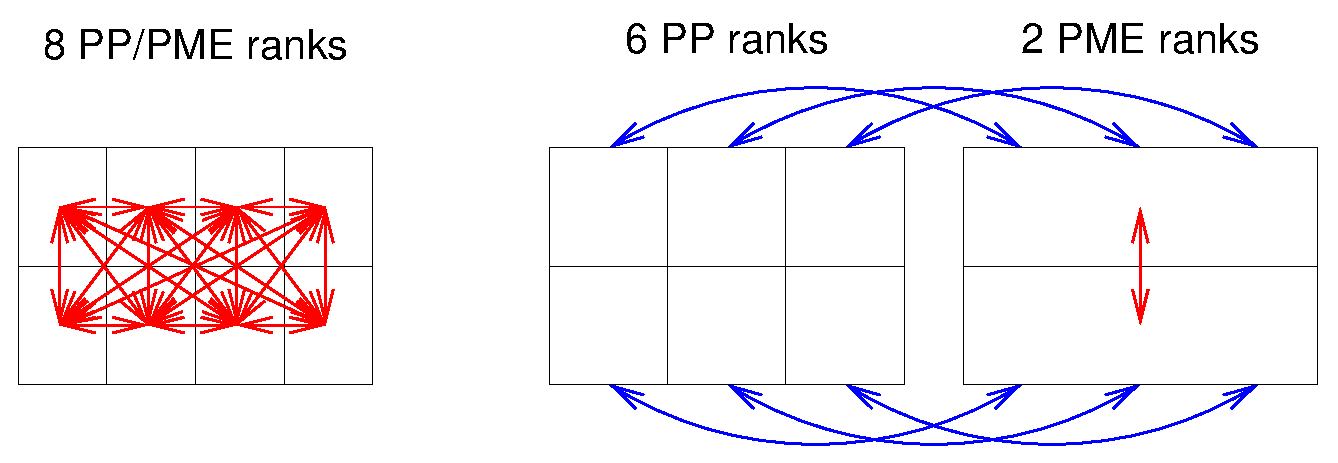
\includegraphics[width=12cm]{plots/mpmd-pme}}
\caption{
Example of 8 ranks without (left) and with (right) MPMD.
The PME communication (red arrows) is much higher on the left
than on the right. For MPMD additional PP - PME coordinate
and force communication (blue arrows) is required,
but the total communication complexity is lower.
\label{fig:mpmd_pme}
}
\end{figure}

{\tt mdrun} will by default interleave the PP and PME ranks.
If the ranks are not number consecutively inside the machines,
one might want to use {\tt mdrun -ddorder pp_pme}.
For machines with a real 3-D torus and proper communication software
that assigns the ranks accordingly one should use
{\tt mdrun -ddorder cartesian}.

To optimize the performance one should usually set up the cut-offs
and the PME grid such that the PME load is 25 to 33\% of the total
calculation load. {\tt grompp} will print an estimate for this load
at the end and also {\tt mdrun} calculates the same estimate
to determine the optimal number of PME ranks to use.
For high parallelization it might be worthwhile to optimize
the PME load with the {\tt mdp} settings and/or the number
of PME ranks with the {\tt -npme} option of {\tt mdrun}.
For changing the electrostatics settings it is useful to know
the accuracy of the electrostatics remains nearly constant
when the Coulomb cut-off and the PME grid spacing are scaled
by the same factor.
{\bf Note} that it is usually better to overestimate than to underestimate
the number of PME ranks, since the number of PME ranks is smaller
than the number of PP ranks, which leads to less total waiting time.

The PME domain decomposition can be 1-D or 2-D along the $x$ and/or
$y$ axis. 2-D decomposition is also known as \normindex{pencil decomposition} because of
the shape of the domains at high parallelization.
1-D decomposition along the $y$ axis can only be used when
the PP decomposition has only 1 domain along $x$. 2-D PME decomposition
has to have the number of domains along $x$ equal to the number of
the PP decomposition. {\tt mdrun} automatically chooses 1-D or 2-D
PME decomposition (when possible with the total given number of ranks),
based on the minimum amount of communication for the coordinate redistribution
in PME plus the communication for the grid overlap and transposes.
To avoid superfluous communication of coordinates and forces
between the PP and PME ranks, the number of DD cells in the $x$
direction should ideally be the same or a multiple of the number
of PME ranks. By default, {\tt mdrun} takes care of this issue.

\subsection{Domain decomposition flow chart}
In \figref{dd_flow} a flow chart is shown for domain decomposition
with all possible communication for different algorithms.
For simpler simulations, the same flow chart applies,
without the algorithms and communication for
the algorithms that are not used.

\begin{figure}
\centerline{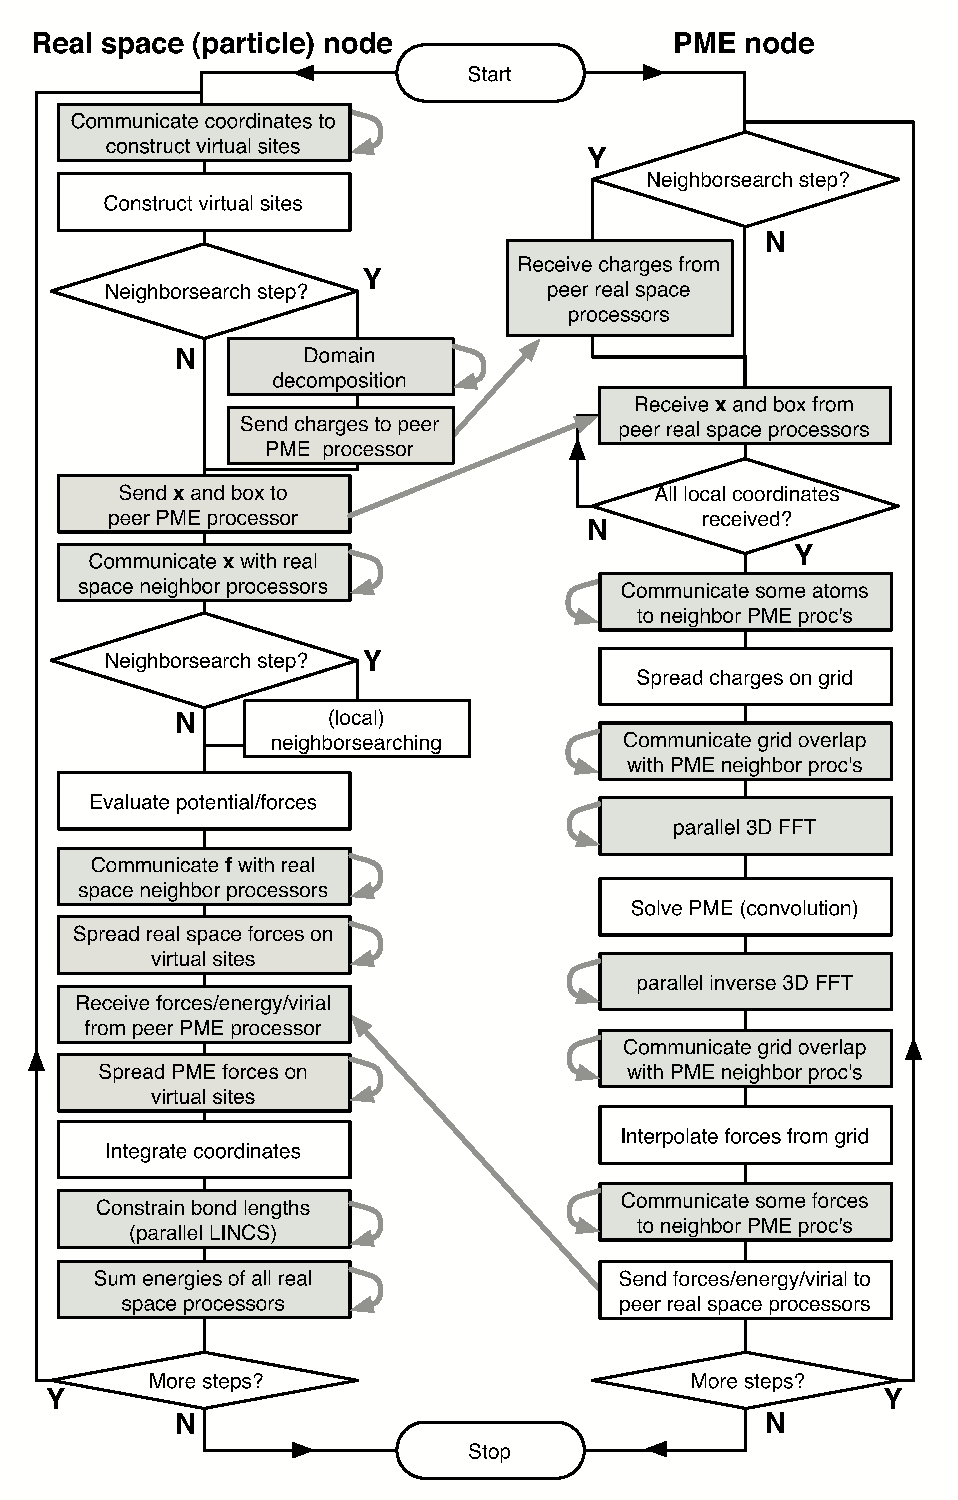
\includegraphics[width=12cm]{plots/flowchart}}
\caption{
Flow chart showing the algorithms and communication (arrows)
for a standard MD simulation with virtual sites, constraints
and separate PME-mesh ranks.
\label{fig:dd_flow}
}
\end{figure}


\section{Implicit solvation\index{implicit solvation}\index{Generalized Born methods}}
\label{sec:gbsa}
Implicit solvent models provide an efficient way of representing 
the electrostatic effects of solvent molecules, while saving a 
large piece of the computations involved in an accurate, aqueous 
description of the surrounding water in molecular dynamics simulations. 
Implicit solvation models offer several advantages compared with 
explicit solvation, including eliminating the need for the equilibration of water 
around the solute, and the absence of viscosity, which allows the protein 
to more quickly explore conformational space.

Implicit solvent calculations in {\gromacs} can be done using the 
generalized Born-formalism, and the Still~\cite{Still97}, HCT~\cite{Truhlar96}, 
and OBC~\cite{Case04} models are available for calculating the Born radii.

Here, the free energy $G_{\mathrm{solv}}$ of solvation is the sum of three terms,
a solvent-solvent cavity term ($G_{\mathrm{cav}}$), a solute-solvent van der
Waals term ($G_{\mathrm{vdw}}$), and finally a solvent-solute electrostatics
polarization term ($G_{\mathrm{pol}}$).

The sum of $G_{\mathrm{cav}}$ and $G_{\mathrm{vdw}}$ corresponds to the (non-polar)
free energy of solvation for a molecule from which all charges
have been removed, and is commonly called $G_{\mathrm{np}}$,
calculated from the total solvent accessible surface area 
multiplied with a surface tension. 
The total expression for the solvation free energy then becomes:

\beq
G_{\mathrm{solv}} = G_{\mathrm{np}}  + G_{\mathrm{pol}}
\label{eqn:gb_solv}
\eeq

Under the generalized Born model, $G_{\mathrm{pol}}$ is calculated from the generalized Born equation~\cite{Still97}:

\beq
G_{\mathrm{pol}} = \left(1-\frac{1}{\epsilon}\right) \sum_{i=1}^n \sum_{j>i}^n \frac {q_i q_j}{\sqrt{r^2_{ij} + b_i b_j \exp\left(\frac{-r^2_{ij}}{4 b_i b_j}\right)}}
\label{eqn:gb_still}
\eeq

In {\gromacs}, we have introduced the substitution~\cite{Larsson10}:

\beq
c_i=\frac{1}{\sqrt{b_i}}
\label{eqn:gb_subst}
\eeq

which makes it possible to introduce a cheap transformation to a new 
variable $x$ when evaluating each interaction, such that:

\beq
x=\frac{r_{ij}}{\sqrt{b_i b_j }} = r_{ij} c_i c_j
\label{eqn:gb_subst2}
\eeq

In the end, the full re-formulation of~\ref{eqn:gb_still} becomes:
 
\beq
G_{\mathrm{pol}} = \left(1-\frac{1}{\epsilon}\right) \sum_{i=1}^n \sum_{j>i}^n \frac{q_i q_j}{\sqrt{b_i  b_j}} ~\xi (x) = \left(1-\frac{1}{\epsilon}\right) \sum_{i=1}^n q_i c_i \sum_{j>i}^n q_j c_j~\xi (x)
\label{eqn:gb_final}
\eeq 

The non-polar part ($G_{\mathrm{np}}$) of Equation~\ref{eqn:gb_solv} is calculated 
directly from the Born radius of each atom using a simple ACE type 
approximation by Schaefer {\em et al.}~\cite{Karplus98}, including a 
simple loop over all atoms. 
This requires only one extra solvation parameter, independent of atom type, 
but differing slightly between the three Born radii models.

% LocalWords:  GROningen MAchine BIOSON Groningen GROMACS Berendsen der Spoel
% LocalWords:  Drunen Comp Phys Comm ROck NS FFT pbc EM ifthenelse gmxlite ff
% LocalWords:  octahedra triclinic Ewald PME PPPM trjconv xy solvated
% LocalWords:  boxtypes boxshapes editconf Lennard COM XTC TNG kT defunits
% LocalWords:  Boltzmann's Mueller nb int mdrun chargegroup simplerc prefactor
% LocalWords:  pme waterloops CH NH CO df com virial integrator Verlet vverlet
% LocalWords:  integrators ref timepoint timestep timesteps mdp md vv avek NVE
% LocalWords:  NVT off's leapfrogv lll LR rmfast SPC fs Nos physicality ps GMX
% LocalWords:  Tcoupling nonergodic thermostatting NOSEHOOVER algorithmes ij yx
% LocalWords:  Parrinello Rahman rescales atm anisotropically ccc xz zx yy yz
% LocalWords:  zy zz se barostat compressibilities MTTK NPT Martyna al isobaric
% LocalWords:  Tuckerman vir PV fkT iLt iL Liouville NHC Eq baro mu trj mol bc
% LocalWords:  freezegroup Shannon's polarizability Overhauser barostats iLn KE
% LocalWords:  negligibly thermostatted Tobias  rhombic maxwell et xtc tng TC rlist
% LocalWords:  waals LINCS holonomic plincs lincs unc ang SA Langevin SD amu BD
% LocalWords:  bfgs Broyden Goldfarb Shanno mkT kJ DFLEXIBLE Nocedal diag nmeig
% LocalWords:  diagonalization anaeig nmens covanal ddg feia BT dp dq pV dV dA
% LocalWords:  NpT eq stepsize REMD constrainted website Okabe MPI covar edi dd
% LocalWords:  progman NMR ddcells innerloops ddtric tric dds rdd conf rcon est
% LocalWords:  mb PP MPMD ddorder pp cartesian grompp npme parallelizable edr
% LocalWords:  macromolecule nstlist vacuo parallelization dof indices MBAR AVX
% LocalWords:  TOL numerics parallelized eigenvectors dG parallelepipeds VdW np
% LocalWords:  Coul multi solvation HCT OBC solv cav vdw Schaefer symplectic dt
% LocalWords:  pymbar multinode subensemble Monte solute subst groupconcept GPU
% LocalWords:  dodecahedron octahedron dodecahedra equilibration usinggroups nm
% LocalWords:  topologies rlistlong CUDA GPUs rcoulomb SIMD BlueGene FPUs erfc
% LocalWords:  cutoffschemesupport unbuffered bondeds OpenMP ewald rtol
% LocalWords:  verletdrift peptide RMS rescaling ergodicity ergodic discretized
% LocalWords:  isothermal compressibility isotropically anisotropic iteratively
% LocalWords:  incompressible integrations translational biomolecules NMA PCA
% LocalWords:  Bennett's equilibrated Hamiltonians covariance equilibrate
% LocalWords:  inhomogeneous conformational online other's th
